\chapter{Conception et expérimentation}

\section{Les technologie utilisés}

Afin de realiser notre project, on a besoin d'une arsenal d'outils. \\

\subsection{Les Langues de programmation}
On va utiliser certaines langues de programmations, chacune est visée vers une plate-forme spécifique:
\begin{itemize}
    \item \verb|Dart| avec le \acrshort{SDK} \verb|Flutter|: Utilisé pour la programmation de l'application mobile, on va parfois utiliser autres langages pour modifier quelques caractéristiques natives de l'application mobile qu'on peut pas modifier avec Dart seulement.
    \begin{itemize}
        \item \verb|Java| pour l'Android
        \item \verb|Swift| pour l'IOS
    \end{itemize}
    \item \verb|Html|, \verb|CSS| et \verb|JavaScript|: Pour le site web qui sera partagé par l'utilisateur, on va aussi utiliser la librairie \verb|React.js| avec \verb|TypeScript|.
    \item \verb|Arduino C++|: Pour le développement de l'application de la carte Arduino. Ce dernier semble à C++ standard, avec quelques différences mineures.
\end{itemize}

\begin{figure}[!htbp]
    \centering
    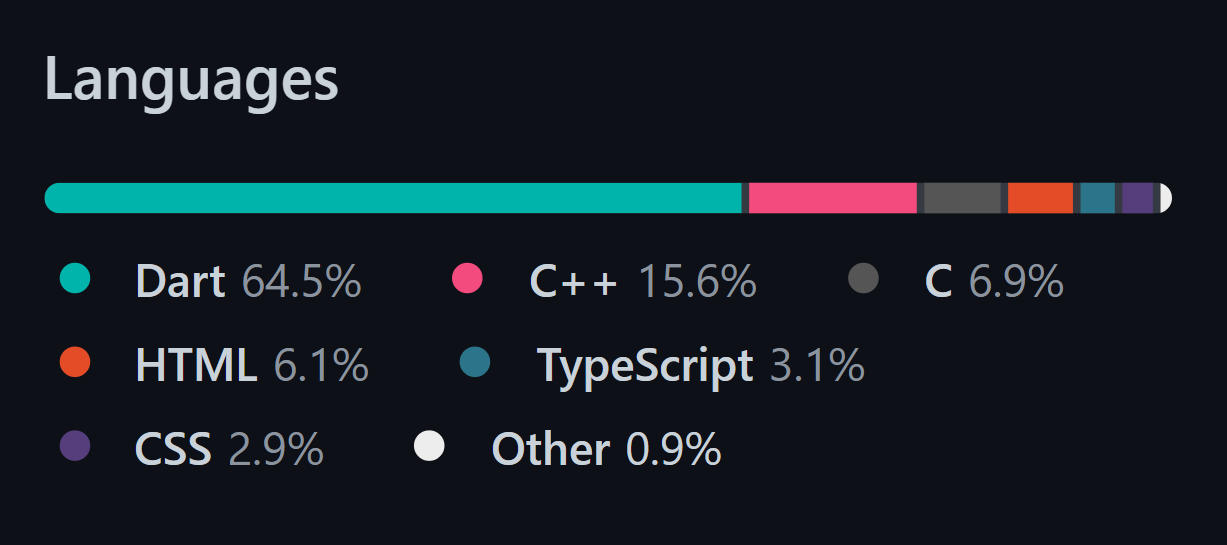
\includegraphics[width=.7\linewidth]{assets/used languages.png}
    \caption{Les différents langues de programmation utilisées}
\end{figure}

\FloatBarrier

\subsection{Les applications et outils}
Juste comme les langues, on a besoin de quelques applications et outils afin de réaliser ce projet.

\begin{itemize}
    \item \verb|Visual Studio Code|: C'est l'éditeur de code de choix. Il est facile, utile, et robuste.
    \item \verb|Arduino| \acrshort{IDE}: Utiliser pour compiler et transférer le code \verb|C++| vers l'Arduino.
    \item \verb|SolidWorks|: Utiliser pour la conception du boîtier de la canne.
    \item \verb|Fritzing|: Pour la modélisation du circuit électrique.
    \item \verb|Proteus PCB|: Pour la réalisation du circuit de la carte imprimée \acrshort{PCB}.
    \item \verb|Desmos|: Pour dessiner les courbes citées dans ce rapport.
\end{itemize}

\subsection{Les services utilisés}

Pour pouvoir chercher des endroits et obtenir leur nom, leur emplacement, leur type, leurs heures d’ouverture..., nous aurons besoin d’une sorte de base de données contenant toutes ces informations, et c’est là que le service Google entre en jeu.

Google offre un vaste éventail de services, mais nous utiliserons trois d’entre eux:
\begin{itemize}
    \item GeoCoding
    \item Find Place
    \item Place Details
\end{itemize}

Malheureusement, aucun de ces services n’est gratuit. Nous devrons donc créer une clé API pour les utiliser. mais autant qu'un étudiant, Google ne vous facture pas si l’utilisation totale est inférieure à 200 dollars.

\bgroup
\def\arraystretch{1.5}%  1 is the default, change whatever you need
\begin{table}
    \centering
    \begin{tabular}{|c|c|}
        \hline
        Service & Prix par 1000 requêtes \\
        \hline
        GeoCoding & \$5 \\
        \hline
        Nearby Search & \$17 \\
        \hline
        Place Details & \$17 \\
        \hline
    \end{tabular}
    \caption{Prix des services Google Places \cite{google-maps-pricing}}
\end{table}
\egroup

Toute communication avec les \acrshort{API} de Google sera fait par \acrshort{HTTP} avec une réponse de format \acrshort{JSON}, mais pour simplicité, parfois on va utiliser des libraires qui facilitent la communication.

%%%%%

\subsubsection{GeoCoding}
GeoCoding (géocodage) est le processus de conversion des adresses (comme « 1600 Amphitheatre Parkway, Mountain View, CA ») en coordonnées géographiques (comme 37.423021 de latitude et -122.083739 de longitude) que vous pouvez utiliser pour placer des marqueurs sur une carte ou positionner la carte.

Pour notre application, on utilisera souvent l'inverse (Reverse GeoCoding) pour convertir des coordonnées géographiques en une adresse lisible par l’humain \cite{google-geocoding-overview}.

Exemple d'une réponse de \verb|Google GeoCoding| des cordonnées:
\begin{itemize}
    \item Latitude: 33.591022
    \item Longitude: 3.591022
\end{itemize}

\begin{code}
\begin{minted}[frame=single,
               framesep=3mm,
               linenos=true,
               xleftmargin=21pt,
               tabsize=4, fontsize=\small]{json}
{
   "address_components": [
      {
         "long_name": "HHR4+CX",
         "short_name": "HHR4+CX",
         "types": ["plus_code"]
      },
      {
         "long_name": "Casablanca",
         "short_name": "Casablanca",
         "types": ["locality", "political"]
      },
      {
         "long_name": "Casablanca-Settat",
         "short_name": "Casablanca-Settat",
         "types": ["administrative_area_level_1", "political"]
      },
      {
         "long_name": "Morocco",
         "short_name": "MA",
         "types": ["country", "political"]
      }
   ],
   "formatted_address": "HHR4+CX Casablanca, Morocco",
   "geometry": {
      "bounds": {
         "northeast": {
            "lat": 33.591125,
            "lng": -7.4425
         },
         "southwest": {
            "lat": 33.591,
            "lng": -7.442625
         }
      },
      "location": {
         "lat": 33.591022,
         "lng": -7.442556000000001
      },
      "location_type": "GEOMETRIC_CENTER",
      "viewport": {
         "northeast": {
            "lat": 33.5924114802915,
            "lng": -7.441213519708498
         },
         "southwest": {
            "lat": 33.5897135197085,
            "lng": -7.443911480291503
         }
      }
   },
   "place_id": "GhIJtpvgm6bLQEARJZhqZi3FHcA",
   "plus_code": {
      "compound_code": "HHR4+CX Casablanca, Morocco",
      "global_code": "8C5JHHR4+CX"
   },
   "types": ["plus_code"]
}
\end{minted}
\caption{Exemple d'une réponse Google GeoCoding}
\end{code}

\subsubsection{Nearby Search}

La recherche à proximité vous permet de rechercher des endroits dans une zone spécifiée. Vous pouvez affiner votre demande de recherche en fournissant des mots clés ou en spécifiant le type de lieu que vous recherchez \cite{google-nearby-search}.

On utilisera cette service pour trouve les endroits à proximité, filtrés par type.

Exemple d'une réponse de \verb|Google Nearby Search|:
\begin{code}
\begin{minted}[frame=single,
               framesep=3mm,
               linenos=true,
               xleftmargin=21pt,
               tabsize=4, fontsize=\small]{json}
{
    "html_attributions": [ ], 
    "next_page_token": "Aap_uECVBJCY8nZXQb9ssfnK_LfkwdVQm...", 
    "results": [
        {
            "business_status": "OPERATIONAL", 
            "geometry": {
                "location": {
                    "lat": -33.8587323, 
                    "lng": 151.2100055
                }, 
                "viewport": {
                    "northeast": {
                        "lat": -33.85739817010727, 
                        "lng": 151.2112278798927
                    }, 
                    "southwest": {
                        "lat": -33.86009782989272, 
                        "lng": 151.2085282201073
                    }
                }
            }, 
            "icon": "https://maps.gstatic.com/mapfiles/place...", 
            "icon_background_color": "#FF9E67", 
            "icon_mask_base_uri": "https://maps.gstatic.com/...", 
            "name": "Cruise Bar", 
            "opening_hours": {
                "open_now": false
            }, 
            "photos": [
                {
                    "height": 575, 
                    "html_attributions": [
                        "<a href=\"https://maps.google.com/m..."
                    ], 
                    "photo_reference": "Aap_uEDnz_WTtjeSoT06...", 
                    "width": 766
                }
            ], 
            "place_id": "ChIJi6C1MxquEmsR9-c-3O48ykI", 
            "plus_code": {
                "compound_code": "46R6+G2 The Rocks, New Sout...", 
                "global_code": "4RRH46R6+G2"
            }, 
            "price_level": 2, 
            "rating": 4.1, 
            "reference": "ChIJi6C1MxquEmsR9-c-3O48ykI", 
            "scope": "GOOGLE", 
            "types": [
                ...
            ], 
            "user_ratings_total": 1184, 
            "vicinity": "Level 1, 2 and 3, Overseas Passenger..."
        }, 
        ...
    ], 
    "status": "OK"
}
\end{minted}
\caption{Exemple d'une réponse Nearby Search}
\end{code}

La réponse contient une liste contenant des informations à propos endroits à proximité. \\
Chaque endroit a un champ nommé \verb|place_id|,  c'est l'un qu'on va utiliser pour demander plus d'information a propos ce dernier.

\subsubsection{Place Details}
\label{place-details}

Une fois que vous avez un \verb|place_id| à partir d’une recherche de place, vous pouvez demander plus de détails sur un établissement particulier ou un point d’intérêt en lançant une demande de détails de place. \\
Une demande de Place Details renvoie des informations plus complètes sur le lieu indiqué, telles que son adresse complète, numéro de téléphone, la note de l’utilisateur et les commentaires \cite{google-place-details}.

Exemple d'une réponse de \verb|Google Place Details|:
\begin{code}
\begin{minted}[frame=single,
               framesep=3mm,
               linenos=true,
               xleftmargin=21pt,
               tabsize=4, fontsize=\small]{json}
{
   "html_attributions":[
      
   ],
   "result":{
      "address_components":[
         {
            "long_name":"48",
            "short_name":"48",
            "types":[
               "street_number"
            ]
         },
         ...
      ],
      "adr_address":"<span class=\"street-address\">48 Pirrama Rd</s...",
      "business_status":"OPERATIONAL",
      "formatted_address":"48 Pirrama Rd, Pyrmont NSW 2009, Australia",
      "formatted_phone_number":"(02) 9374 4000",
      "geometry":{
         "location":{
            "lat":-33.866489,
            "lng":151.1958561
         },
         "viewport":{
            "northeast":{
               "lat":-33.8655112697085,
               "lng":151.1971156302915
            },
            "southwest":{
               "lat":-33.86820923029149,
               "lng":151.1944176697085
            }
         }
      },
      "icon":"https://maps.gstatic.com/mapfiles/place_api/...",
      "icon_background_color":"#7B9EB0",
      "icon_mask_base_uri":"https://maps.gstatic.com/mapfi...",
      "international_phone_number":"+61 2 9374 4000",
      "name":"Google Workplace 6",
      "opening_hours":{
         "open_now":false,
         "periods":[
            {
               "close":{
                  "day":1,
                  "time":"1700"
               },
               "open":{
                  "day":1,
                  "time":"0900"
               }
            },
            ...
         ],
         "weekday_text":[
            "Monday: 9:00 AM – 5:00 PM",
            ...
         ]
      },
      "photos":[
         {
            "height":3024,
            "html_attributions":[
               "<a href=\"https://maps.google.com/maps/co..."
            ],
            "photo_reference":"Aap_uECTSiFbO2Qg81vEQkbLMh...",
            "width":4032
         },
         ...
      ],
      "place_id":"ChIJN1t_tDeuEmsRUsoyG83frY4",
      "plus_code":{
         "compound_code":"45MW+C8 Pyrmont NSW, Australia",
         "global_code":"4RRH45MW+C8"
      },
      "rating":4.1,
      "reference":"ChIJN1t_tDeuEmsRUsoyG83frY4",
      "reviews":[
         {
            "author_name":"Mark Smith (Mark ZZZ Smith)",
            "author_url":"https://www.google.com/maps/con...",
            "language":"en",
            "profile_photo_url":"https://lh3.googleuserco...",
            "rating":5,
            "relative_time_description":"a year ago",
            "text":"Great place to visit, cafeteria great...",
            "time":1589072760
         },
         ...
      ],
      "types":[
         ...
      ],
      "url":"https://maps.google.com/?cid=10281119596374313554",
      "user_ratings_total":932,
      "utc_offset":600,
      "vicinity":"48 Pirrama Road, Pyrmont",
      "website":"http://google.com/"
   },
   "status":"OK"
}
\end{minted}
\caption{Exemple d'une réponse Place Details}
\end{code}

%%%%%

\section{La communication Bluetooth}

Avant de commencer à réaliser les taches requis, on doit tout d'abord établir une connexion Bluetooth entre la canne et le téléphone.

\begin{figure}[!htbp]
    \centering
    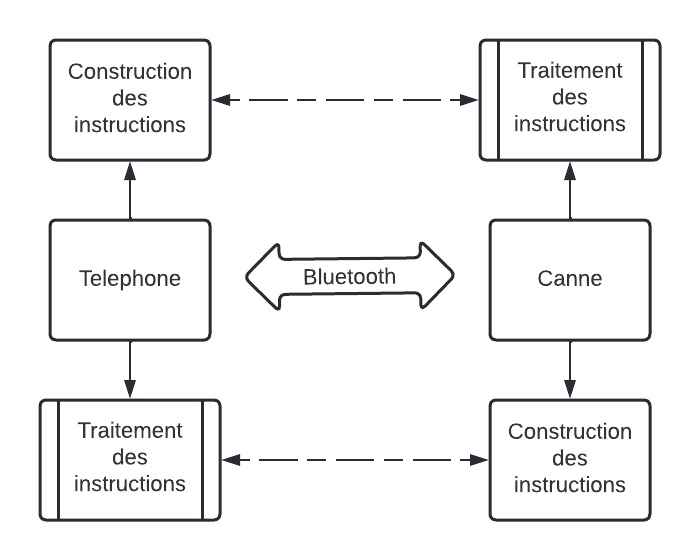
\includegraphics[width=.7\linewidth]{assets/bluetooth/logigramme generale simplifie.png}
    \caption{Logigramme simplifié de la communication Bluetooth}
\end{figure}

\FloatBarrier

\subsection{Établissions de la connexion}

\subsubsection{Au niveau du téléphone}
On doit tout d'abord établir une connexion Bluetooth au périphérique HC-05, pour simplifier un peu les chose, on utilise la librairie \verb|flutter_bluetooth_serial| \cite{flutter_bluetooth_serial}, puis en enregistre un auditeur des évènements qui traite chaque instruction reçue via Bluetooth.

\begin{code}
\begin{minted}[frame=single,
               framesep=3mm,
               linenos=true,
               xleftmargin=21pt,
               tabsize=4, fontsize=\small, breaklines]{dart}
BluetoothConnection? _connection;
bool isConnected = false;
void connect() async {
    const String address = "98:D3:33:81:3D:33"; // L'adresse MAC
    try {
      _connection = await BluetoothConnection.toAddress(address);
      isConnected = true;
      _connection?.input?.listen(_onRecievePayload);
    } catch (exception) {
      isConnected = false;
    }
  }
\end{minted}
\caption{Connecter le téléphone à HC-05}
\end{code}

La fonction \verb|_onRecievePayload| sera responsable du la lecture de l'emport Bluetooth.

\subsubsection{Au niveau de la canne}
Au niveau de la canne c'est très simple à se connecter avec le HC-05, puisque c'est une communication série, on peut utiliser la librairie SoftwareSerial.

\begin{code}
\begin{minted}[frame=single,
               framesep=3mm,
               linenos=true,
               xleftmargin=21pt,
               tabsize=4, fontsize=\small, breaklines]{cpp}
#include <SoftwareSerial.h>

namespace Bluetooth
{
    SoftwareSerial BTSerial(4, 3); // TXD | RXD
}
\end{minted}
\caption{Connecter le canne à HC-05}
\end{code}

On peut utiliser les fonctions disponibles juste comme c'était l'interface \verb|Serial|, par exemple:
\begin{itemize}
    \item \verb|BTSerial.print| pour écrire
    \item \verb|BTSerial.read| pour lire
    \item \dots
\end{itemize}

\begin{figure}[!htbp]
    \centering
    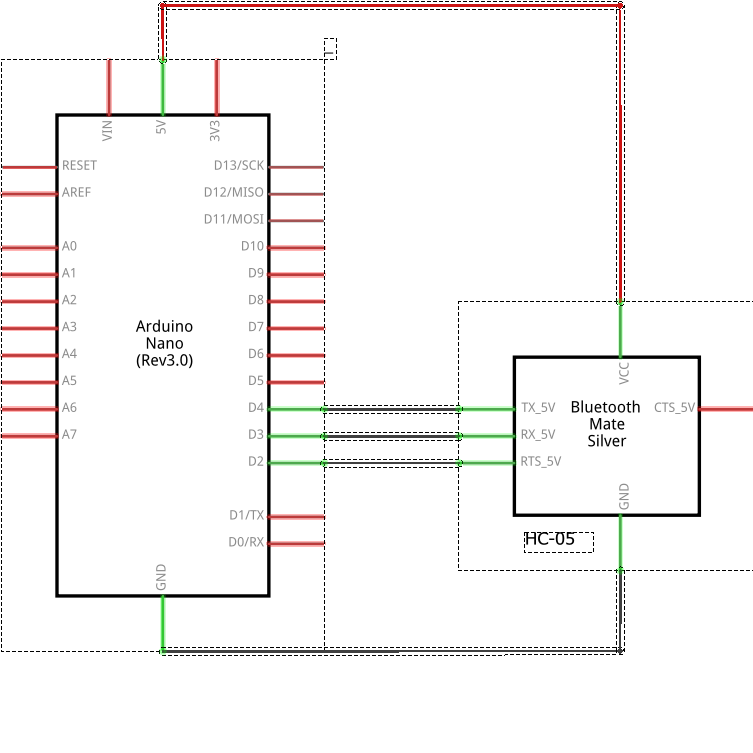
\includegraphics[width=.7\linewidth]{assets/HC-05/circuit.png}
    \caption{Schéma de montage de HC-05 avec l'arduino}
\end{figure}

\FloatBarrier

\subsection{Lecture Traitement des instructions}

Le traitement des instructions est séparé en deux parties:
\begin{itemize}
    \item Lecture de l'emport (Payload)
    \item Traitement de l'instruction
\end{itemize}

Avant de commencer, on doit d'abord définir la format et une liste des instructions qui seront utilisés.

\textbf{Format:} \verb$INSTRUCTION:ARG1|ARG2|ARG3|...$

\bgroup
\def\arraystretch{1.5}
\begin{table}[!htbp]
    \centering
    \begin{tabular}{|C{6cm}|C{2cm}|C{2cm}|C{6.3cm}|}
        \hline
        Instruction & Envoyée par & Paramètres & Description \\
        \hline
        \verb|SEND_LOCATION_SMS| & Canne & - & Envoyer l'SMS d'urgence \\
        \hline
        \verb|BATTERY_PERCENTAGE| & Canne & pourcentage & Mettre à jour la valeur de la batterie \\
        \hline
        \verb|RING| & Téléphone & - & Lancer la sonnerie de la canne \\
        \hline
        \verb|RING| & Canne & - & Lancer la sonnerie du téléphone \\
        \hline
        \verb|SPEAK| & Canne & phrase & synthèse vocale \\
        \hline
        \verb|NAVIGATABLES:NEXT| & Canne & - & Naviguer au bouton suivant \\
        \hline
        \verb|NAVIGATABLES:PREVIOUS| & Canne & - & Naviguer au bouton précédent \\
        \hline
        \verb|NAVIGATABLES:BACK| & Canne & - & Retourner à la page précédente \\
        \hline
        \verb|NAVIGATABLES:PRESS| & Canne & - & Cliquer le bouton sélectionné \\
        \hline
        \verb|NAVIGATABLES:RESET| & Canne & - & Redémarrer l'application \\
        \hline
        \verb|NAVIGATABLES:EXPLORE| & Canne & - & Naviguer à la page "Explore" \\
        \hline
    \end{tabular}
    \caption{Liste des instructions Bluetooth}
    \label{bluetooth-commandes}
\end{table}
\egroup

\FloatBarrier

\subsubsection{Lecture de l'emport}
La communication Bluetooth est une communication série, donc on doit séparer chaque instruction de l'autre, d'où on doit fixer un caractère qui va signifier que l'instruction est terminée. \\
On a choisi le character \verb|\n| (End of line character) qui est deja le standard, son code \acrshort{ASCII} est 0x10.

\begin{figure}[!htbp]
    \centering
    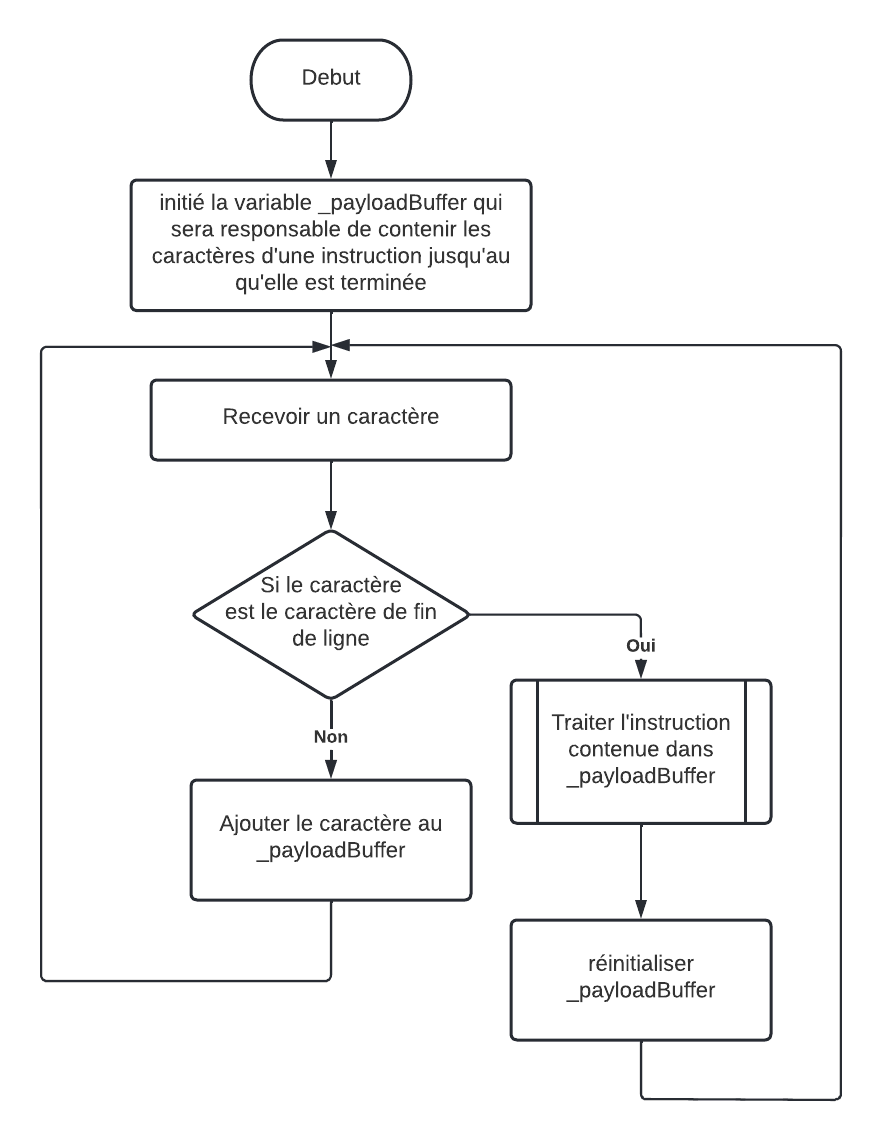
\includegraphics[width=.7\linewidth]{assets/bluetooth/read payload.png}
    \caption{Logigramme de lecture du Payload Bluetooth}
\end{figure}

\FloatBarrier

\paragraph{Au niveau du téléphone}

\begin{code}
\begin{minted}[frame=single, framesep=3mm, linenos=true, xleftmargin=21pt, tabsize=4, fontsize=\small, breaklines]{dart}
void _onRecievePayload(Uint8List payload) {
    for (var char in payload) {
        // 0x0A (10) corresponds to \n char
        if (char == 0x0A) {
            parseBluetoothPayload(_payloadBuffer);
            _payloadBuffer = ""; // Reset Message buffer
        } else {
            _payloadBuffer += ascii.decode([char]);
        }
    }
}    
\end{minted}
\caption{Lecture du Payload Bluetooth au niveau de l'application mobile}
\end{code}

\paragraph{Au niveau de la canne}

\begin{code}
\begin{minted}[frame=single, framesep=3mm, linenos=true, xleftmargin=21pt, tabsize=4, fontsize=\small, breaklines]{cpp}
if (BTSerial.available()) {
    int thisChar = BTSerial.read();
    if (thisChar == 0xA) {
            parsePayload(_payloadBuffer); // Parse payload
            _payloadBuffer = "";          // Reset payload buffer
    } else {
        _payloadBuffer += ((char)thisChar); // Add current char to payloadBuffer after casting
    }
}        
\end{minted}
\caption{Lecture du Payload Bluetooth au niveau de l'Arduino}
\end{code}

Les fonctions \verb|parsePayload| (pour la canne) et \verb|parseBluetoothPayload|  (pour l'application mobile) seront responsable du traitement des instructions Bluetooth

\subsubsection{Traitement de l'instruction}
Pour traiter l'instruction, on doit tout d'abord la séparer pour avoir le non de l'instruction et ses arguments. Le code se diffère beaucoup entre \verb|C++| et \verb|Dart| où il est plus facile a l'implémenter avec \verb|Dart|.

Nous suivons un modèle de programmation orienté objet; d'où, chaque tache aura son propre gestionnaire qui hérite les méthodes de traitement de son classe parent.

\paragraph{Au niveau du téléphone}

\begin{code}
\begin{minted}[frame=single, framesep=3mm, linenos=true, xleftmargin=21pt, tabsize=4, fontsize=\small, breaklines]{dart}
abstract class BluetoothPayloadHandler {
  late String command;
  void handle(List<String> args);
}  
\end{minted}
\caption{Classe gestionnaire d'instruction parent de l'application mobile}
\end{code}

\begin{code}
\begin{minted}[frame=single, framesep=3mm, linenos=true, xleftmargin=21pt, tabsize=4, fontsize=\small, breaklines]{dart}
void parseBluetoothPayload(String payload) {
  print(payload);

  final String command = payload.split(":").first;

  final List<String> args =
      payload.split(":").length == 2 ? payload.split(":").elementAt(1).split("|") : [];

  final List<BluetoothPayloadHandler> _handlers = [
    SendCurrentLocationSMS(),
    UpdateCaneBatteryPercentage(),
    StartPhoneRingtone(),
    Speak(),
    NavigatablesRemote(),
  ];

  for (var handler in _handlers) {
    if (handler.command == command) handler.handle(args);
  }
}
\end{minted}
\caption{Traiteur du Payload Bluetooth de l'application mobile}
\end{code}

\paragraph{Au niveau de la canne}

\begin{code}
\begin{minted}[frame=single, framesep=3mm, linenos=true, xleftmargin=21pt, tabsize=4, fontsize=\small, breaklines]{cpp}
class BluetoothHandler
{
public:
    String command;
    void (*handle)(String[], int);

    BluetoothHandler(
        String _command,
        void (*_handle)(String[], int))
    {
        command = _command;
        handle = _handle;
    }
};
\end{minted}
\caption{Classe gestionnaire d'instruction parent de la canne}
\end{code}

\begin{code}
\begin{minted}[frame=single, framesep=3mm, linenos=true, xleftmargin=21pt, tabsize=4, fontsize=\small, breaklines]{cpp}
void parsePayload(String payload) {
    int indexOfDoublePoints = payload.indexOf(":");
    String command = payload.substring(0, indexOfDoublePoints);
    String argsString = payload.substring(indexOfDoublePoints + 1);
    String args[] = {};
    int argsLength = 0;
    int indexOfPipe = -1;
    int currentPipeSearchIndex = 0;

    do {
        indexOfPipe = argsString.substring(currentPipeSearchIndex).indexOf("|");
        String arg = argsString.substring(currentPipeSearchIndex, indexOfPipe);
        currentPipeSearchIndex += arg.length() + 1;
        args[argsLength] = arg;
        argsLength++;
    } while (indexOfPipe != -1);

    for (int i = 0; i < _handlersCount; i++) {
        BluetoothHandler handler = _handlers[i];
        if (handler.command == command) {
            handler.handle(args, argsLength);
            break;
        }
    }
}
\end{minted}
\caption{Traiteur du Payload Bluetooth de la canne}
\end{code}

\subsection{L'envoie d'une instruction}

Pour envoyer une instruction, on doit la mettre en forme

\subsubsection{Au niveau de la canne}
\begin{code}
\begin{minted}[frame=single, framesep=3mm, linenos=true, xleftmargin=21pt, tabsize=4, fontsize=\small, breaklines]{cpp}
void send(String command, String args[], int length) {
    String payload = command + ":";

    for (int i = 0; i < length; i++) {
        payload += args[i];
        if (i != (length - 1)) // Add pipe char (|) between args
            payload += "|";
    }
    
    payload += ((char)0x0A); // Add \n char
    BTSerial.print(payload); // Send payload
}
\end{minted}
\caption{Envoyer une instruction d'après la canne}
\end{code}

\subsubsection{Au niveau de l'application mobile}
\begin{code}
\begin{minted}[frame=single, framesep=3mm, linenos=true, xleftmargin=21pt, tabsize=4, fontsize=\small, breaklines]{dart}
void send(String command, List<String> args) {
    String payload = command + ":" + args.join("|");
    _sendPayload(payload);
}

void _sendPayload(String payload) {
    _connection?.output.add(
      Uint8List.fromList([...ascii.encode(payload), 0x0A]),
    );
}
\end{minted}
\caption{Envoyer une instruction au niveau de l'application mobile}
\end{code}

%%%%%

\section{Feedback (rétroaction)}

Comme l’utilisateur a une déficience visuelle, il n’aura aucune idée si la commande qu’il a demandée a été exécutée ou non, puisque nous devons lui fournir un certain type de rétroaction, et nous avons fait les trois.
\begin{itemize}
    \item Visual feedback (rétroaction visuelle)
    \item Audible feedback (rétroaction audio)
    \item Vocal feedback (rétroaction vocale)
\end{itemize}

\subsection{Visual feedback}
Le visuel ne cible pas directement l’utilisateur malvoyant, c’est un signe pour les autres. \\
Il y aurait 3 \acrshort{LED}s, de couleurs différentes:
\begin{itemize}
    \item Blanche : pour rendre l’utilisateur plus visible lors de la navigation dans la nuit, pour éviter de ne pas être vu.
    \item Verte: Pour indiquer que la canne est allumée
    \item Rouge: Pour indiquer que la batterie est déchargé (moins de 20\%)
\end{itemize}

Les \acrshort{LED}s sont connectés à l'Arduino selon ce schéma:

\begin{figure}[!htbp]
    \centering
    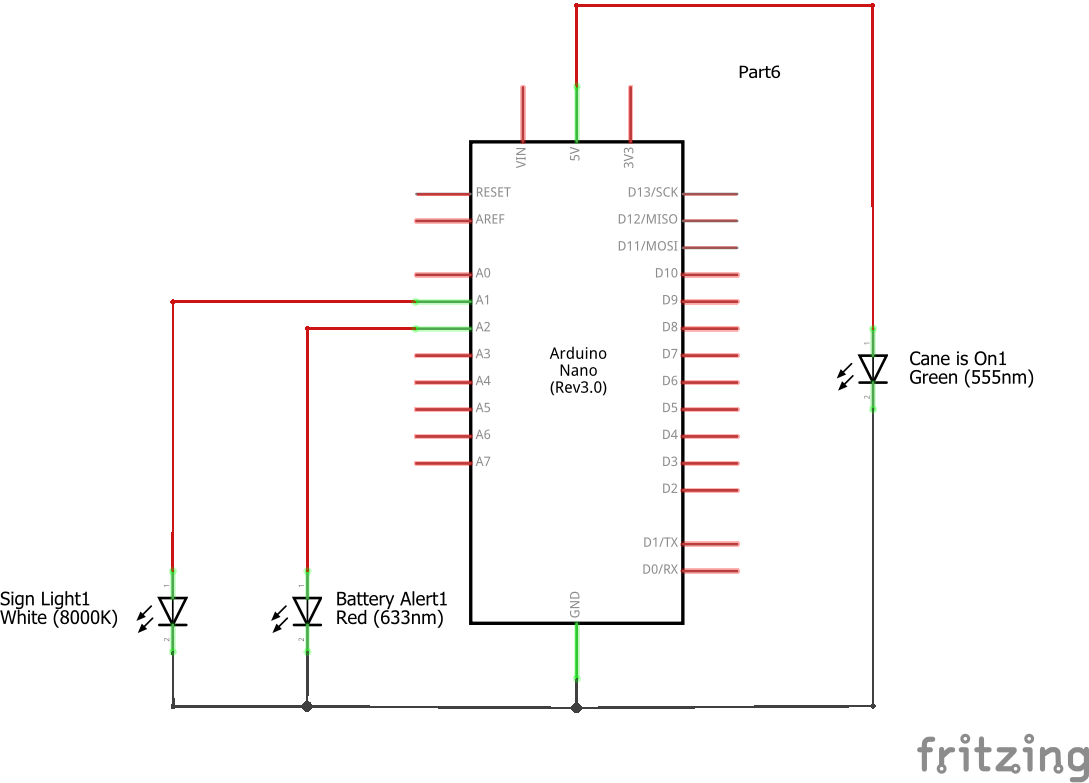
\includegraphics[width=\linewidth]{assets/leds circuit.png}
    \caption{Schéma de montage des \acrshort{LED}s avec l'Arduino}
\end{figure}

\FloatBarrier

On a utilisé les broches d'entrée analogue d'Arduino (Ax) puisque les autres broches (Dx) ont manqué. Les porte A0 à A4 peut être utilisé comme sortie logique sans aucun problème

\subsection{Audible feedback}
En utilisant le Buzzer dont nous avons parlé au chapitre \ref{buzzer}, nous pouvons jouer une sonnerie à l’aide de la fonction Arduino \verb|tone| \cite{arduino-tone}.

Le bipeur doit être connecter à une broche de sortie \acrshort{PWM}, on a choisi la broche 11.

\begin{figure}[!htbp]
    \centering
    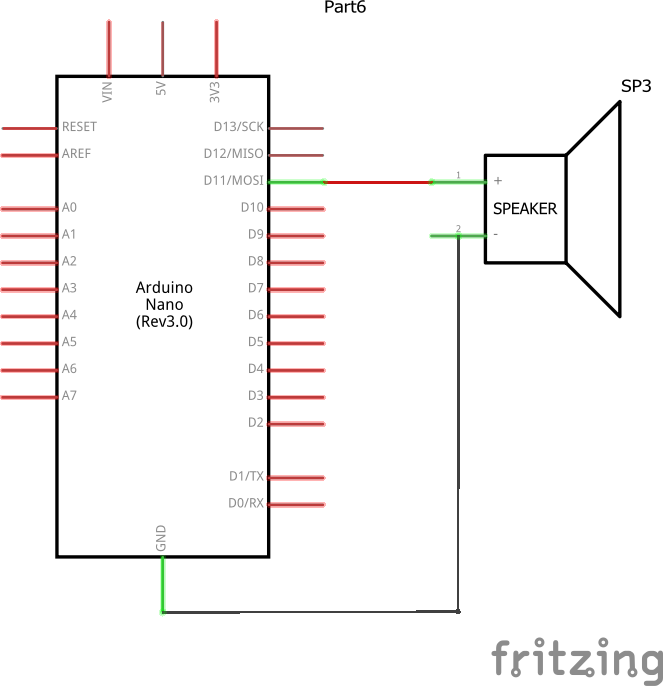
\includegraphics[width=.6\linewidth]{assets/buzzer circuit.png}
    \caption{Schéma de montage de bipeur avec l'Arduino}
\end{figure}

\FloatBarrier

On doit aussi déclarer des mélodie qui seront joue par le bipeur, puisque nous suivons un modèle de programmation \acrshort{OOP}, on va déclarer un Classe \verb|Melody|, est une liste des mélodies disponibles.
Ces mélodies seront jouées lors de:
\begin{itemize}
    \item Une clique de bouton (Ça diffère d'un type de clique a l'autre)
    \item La sonnerie de la canne
    \item Le démarrage de la canne
\end{itemize}

\begin{code}
\begin{minted}[frame=single, framesep=3mm, linenos=true, xleftmargin=21pt, tabsize=4, fontsize=\small, breaklines]{cpp}
#include "./pitches.h" // Maps each note to its frequency

class Ringtone {
public:
    static const int MAX_LENGTH = 100;
    const int *notes;
    int length;
    int duration;
    int sleep;

    Ringtone(const int *_notes, int _length, int _duration, int _delay) {
        notes = _notes;
        length = _length;
        duration = _duration;
        sleep = _delay;
    }

    void play() {
        for (int i = 0; i < length; i++) {
            tone(11, notes[i], duration);
            delay(sleep);
        }
    }
};

namespace Ringtones {
    const int startupMelody[] = {NOTE_E6, NOTE_C7, NOTE_A6, NOTE_B6};
    Ringtone startup(startupMelody, 4, 200, 150);

    const int ringtoneMelody[] = {NOTE_A7, NOTE_D7};
    Ringtone ringtone(ringtoneMelody, 2, 250, 150);

    const int buttonClickMelody[] = {0, NOTE_E6, 0};
    Ringtone buttonClick(buttonClickMelody, 3, 150, 100);

    const int buttonDoubleClickMelody[] = {0, NOTE_F5, 0};
    Ringtone buttonDoubleClick(buttonDoubleClickMelody, 3, 150, 100);

    const int buttonLongClickMelody[] = {0, NOTE_CS6, 0};
    Ringtone buttonLongClick(buttonLongClickMelody, 3, 150, 100);
}
\end{minted}
\caption{Ringtone}
\end{code}

\subsection{Vocal feedback}
Nous voulions inclure la rétroaction vocale dans la canne elle-même, mais malheureusement, les données vocales prennent trop d’espace, ce que Arduino n’a pas beaucoup d’espace (32 Ko), alors nous avons décidé d’utiliser le téléphone comme un middleware pour jouer les phrases vocales.

Les instructions seront envoyées par la canne en utilisant l'instruction Bluetooth \verb|SPEAK| comme décrit dans ce tableau \ref{bluetooth-commandes}

\subsubsection*{Screen readers (Lecteurs d'écran)}
Un lecteur d’écran est une technique d’assistance, principalement utilisée par les personnes ayant une déficience visuelle. Il convertit du texte, des boutons, des images et d’autres éléments d’écran en discours ou en braille. Voyons ce qu’est un lecteur d’écran, comment il fonctionne et voyons les aveugles en action! \cite{what-is-screen-reader}.
%%%%%

\section{Les boutons de commande}

Afin de commander le téléphone à distance, on aura besoin de quelque sort d'une interface de commande, d'où on a choisi d'utiliser 5 boutons poussoirs situés sur la canne. \\
Nous aurons 9 instructions qu'on doit traiter, d'où on aura besoin de trouver une méthode pour traiter 9 différents tâches, avec que 5 boutons. \\
Donc chaque boutons aura la possibilité d'exécuter deux différents tâches dépendant sur le type de la clique, d'une totalité de 10 tâches.
\begin{itemize}
    \item Clique simple
    \item Clique lente
\end{itemize}

On a aussi ajouter un autre type, au cas on a voulu ajouter plus de tâches.
\begin{itemize}
    \item Double clique
\end{itemize}

\begin{code}
\begin{minted}[frame=single, framesep=3mm, linenos=true, xleftmargin=21pt, tabsize=4, fontsize=\small, breaklines]{cpp}

#include <Arduino.h>

#include "../../includes/ringtones.cpp"

class Button {
public:
    // All times are in ms
    unsigned long singlePressPolling = 1000;
    unsigned long doublePressTimeout = 250;
    unsigned long longPressTriggerTimeout = 1000;
    unsigned long minPressPolling = 10;

private:
    int _port;
    bool _prevState = false;
    bool _currentState = false;
    bool _singlePressInQueue = false;
    bool _longPressInProgress = false;
    unsigned long _lastPressedAt = 0;

    // Handlers
    void (*_onPress)();
    void (*_onDoublePress)();
    void (*_onLongPress)();

    static void _defaultHandler() {}

public:
    Button(
        int port,
        void (*onPress)(),
        void (*onDoublePress)() = _defaultHandler,
        void (*onLongPress)() = _defaultHandler
    ) {
        _port = port;
        _onPress = onPress;
        _onDoublePress = onDoublePress;
        _onLongPress = onLongPress;

        pinMode(port, INPUT_PULLUP);
    }

    void listen() {
        _currentState = !(bool)digitalRead(_port);

        if (millis() < _lastPressedAt + minPressPolling)
            return;

        if (_singlePressInQueue) {
            if (_currentState && _prevState) {
                if (millis() >= _lastPressedAt + longPressTriggerTimeout) {
                    handleLongPress();
                    _singlePressInQueue = false;
                    _longPressInProgress = false;
                    _lastPressedAt = millis();
                }
            } else if (millis() <= _lastPressedAt + doublePressTimeout && _currentState && !_prevState) {
                handleDoublePress();
                _singlePressInQueue = false;
                _lastPressedAt = millis();
            } else if (millis() > _lastPressedAt + doublePressTimeout) {
                handlePress();
                _singlePressInQueue = false;
                _lastPressedAt = millis();
            }
        } else if (millis() >= _lastPressedAt + singlePressPolling && _currentState && !_prevState) {
            _singlePressInQueue = true;
            _longPressInProgress = false;
            _lastPressedAt = millis();
        }

        _prevState = _currentState;
    }

private:
    void handlePress() {
        Ringtones::buttonClick.play();
        _onPress();
    }

    void handleDoublePress() {
        Ringtones::buttonDoubleClick.play();
        _onDoublePress();
    }

    void handleLongPress() {
        Ringtones::buttonLongClick.play();
        _onLongPress();
    }
};
\end{minted}
\caption{Button}
\end{code}

\bgroup
\def\arraystretch{1.5}%  1 is the default, change whatever you need
\begin{table}[!htbp]
    \centering
    \begin{tabular}{|C{1.7cm}|C{5cm}|C{1.7cm}|C{5cm}|}
        \hline
        Bouton & Clique simple & Double clique & Clique lente \\
        \hline
        Milieu & - & - & Cliquer le bouton sélectionné \\
        \hline
        Gauche & Naviguer au bouton précédent & - & Envoyer l'SMS d'urgence \\
        \hline
        Droite & Naviguer au bouton suivant & - & Naviguer à la page "Explore" \\
        \hline
        Haut & Retourner à la page précédente & - & Redémarrer l’application \\
        \hline
        Bas & Cliquer le bouton sélectionné & - & Lancer la sonnerie du téléphone \\
        \hline
    \end{tabular}
    \caption{Cartographie des boutons}
\end{table}
\egroup

\section{Les taches intelligents réalisés sur la canne}

\subsection{La détection d’obstacles}

\subsubsection{Montage}
On connecte le capteur de proximité HC-SR04 avec l'arduino suivant le schéma suivant:
\begin{itemize}
    \item VCC $\rightarrow$ 5V
    \item GND $\rightarrow$ GND
    \item TRIG $\rightarrow$ Broche 7
    \item ECHO $\rightarrow$ Broche 8
\end{itemize}

\vspace{18pt}

\begin{figure}[!htbp]
    \centering
    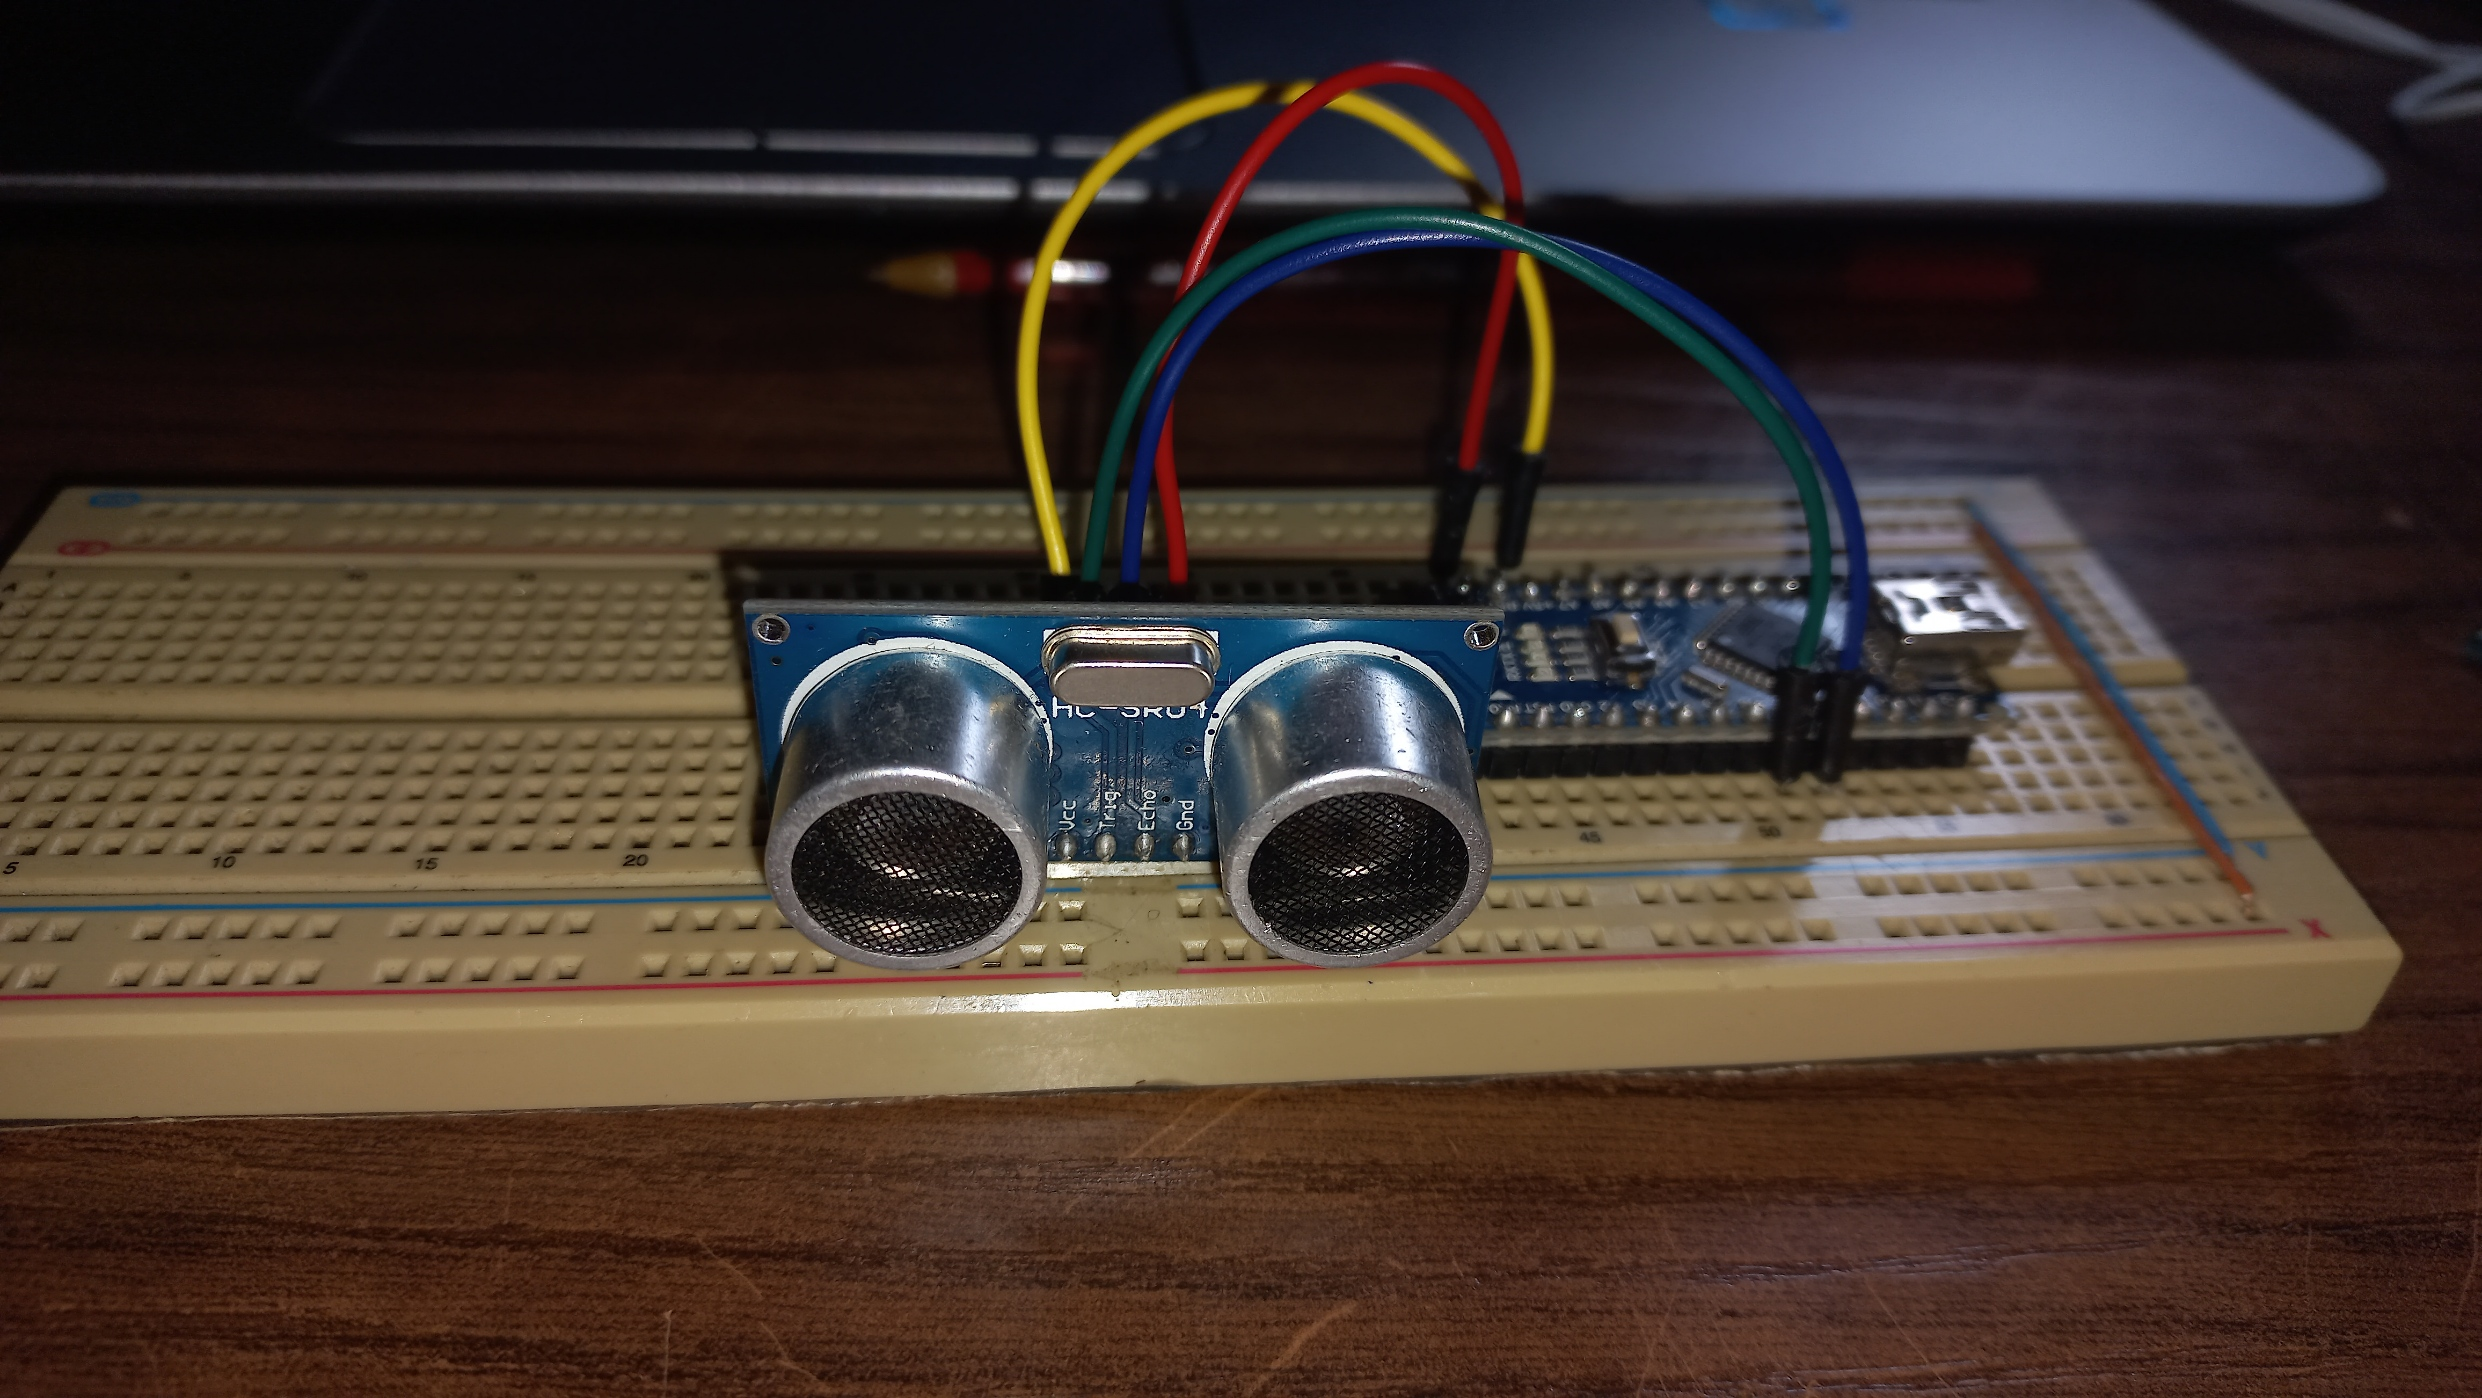
\includegraphics[width=.9\linewidth]{assets/HC-SR04/montage.jpg}
\end{figure}

\begin{figure}[!htbp]
    \centering
    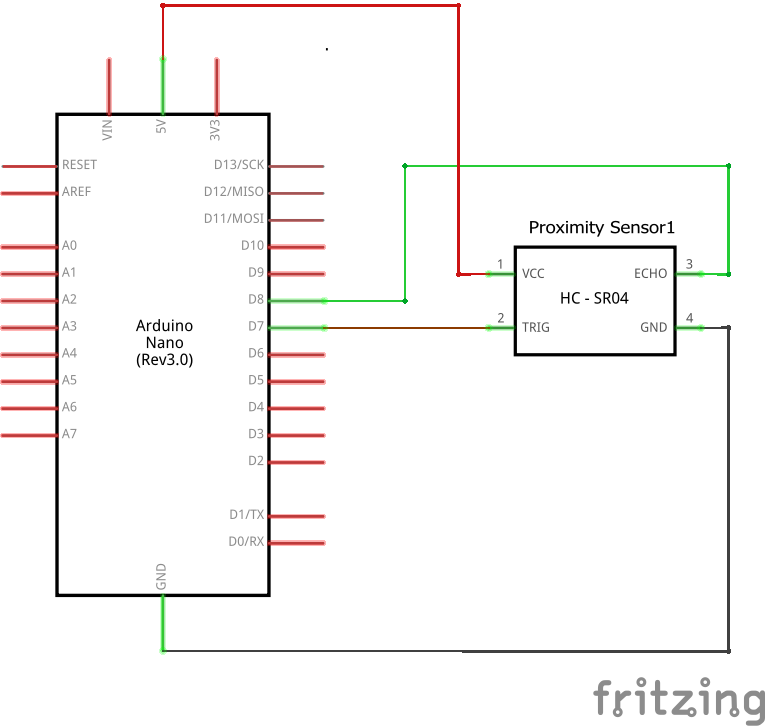
\includegraphics[width=.7\linewidth]{assets/HC-SR04/circuit.png}
    \caption{Schéma et montage de la connexion entre HC-SR04 avec l'arduino}
\end{figure}

\FloatBarrier

\subsubsection{Fonctionnement}
Comme expliqué dans cette paragraphe \fullref{hc-sr04:fonctionnement} du HC-SR04, on doit envoyer un signal d'état haut sur la broche Trigger d'une durée de 10\textmu s, puis la broche Echo va indiquer le temps d'aller-retour pris par le son.

\begin{figure}[!htbp]
    \centering
    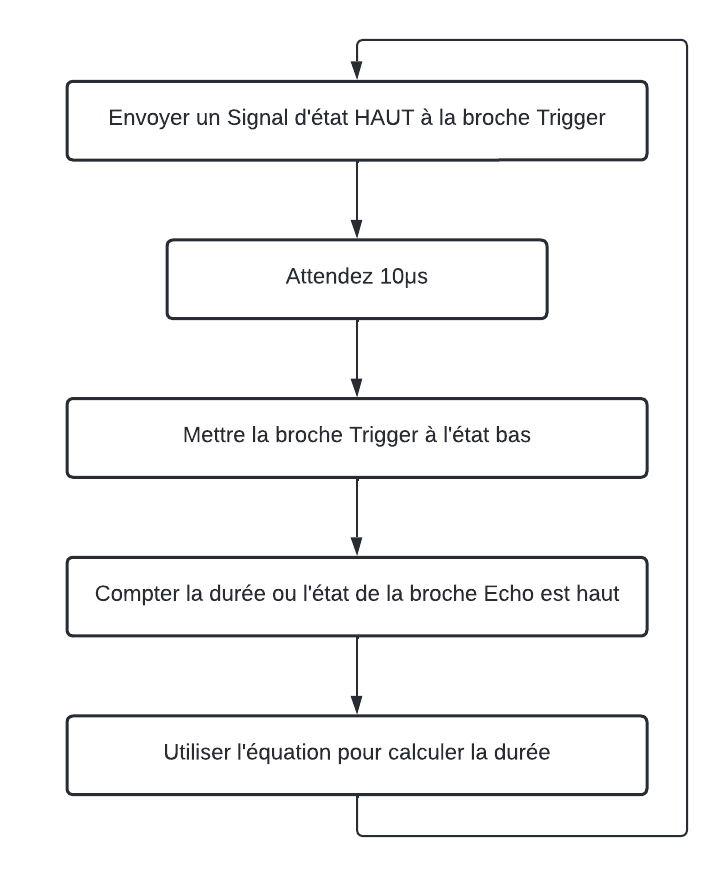
\includegraphics[width=.7\linewidth]{assets/HC-SR04/diagram sans vibration.png}
    \caption{Logigramme du code de HC-SR04}
\end{figure}

% \FloatBarrier

\subsubsection{Des essais}

\begin{figure}
    \centering
    \begin{subfigure}[b]{.4\linewidth}
        \begin{subfigure}{\textwidth}
            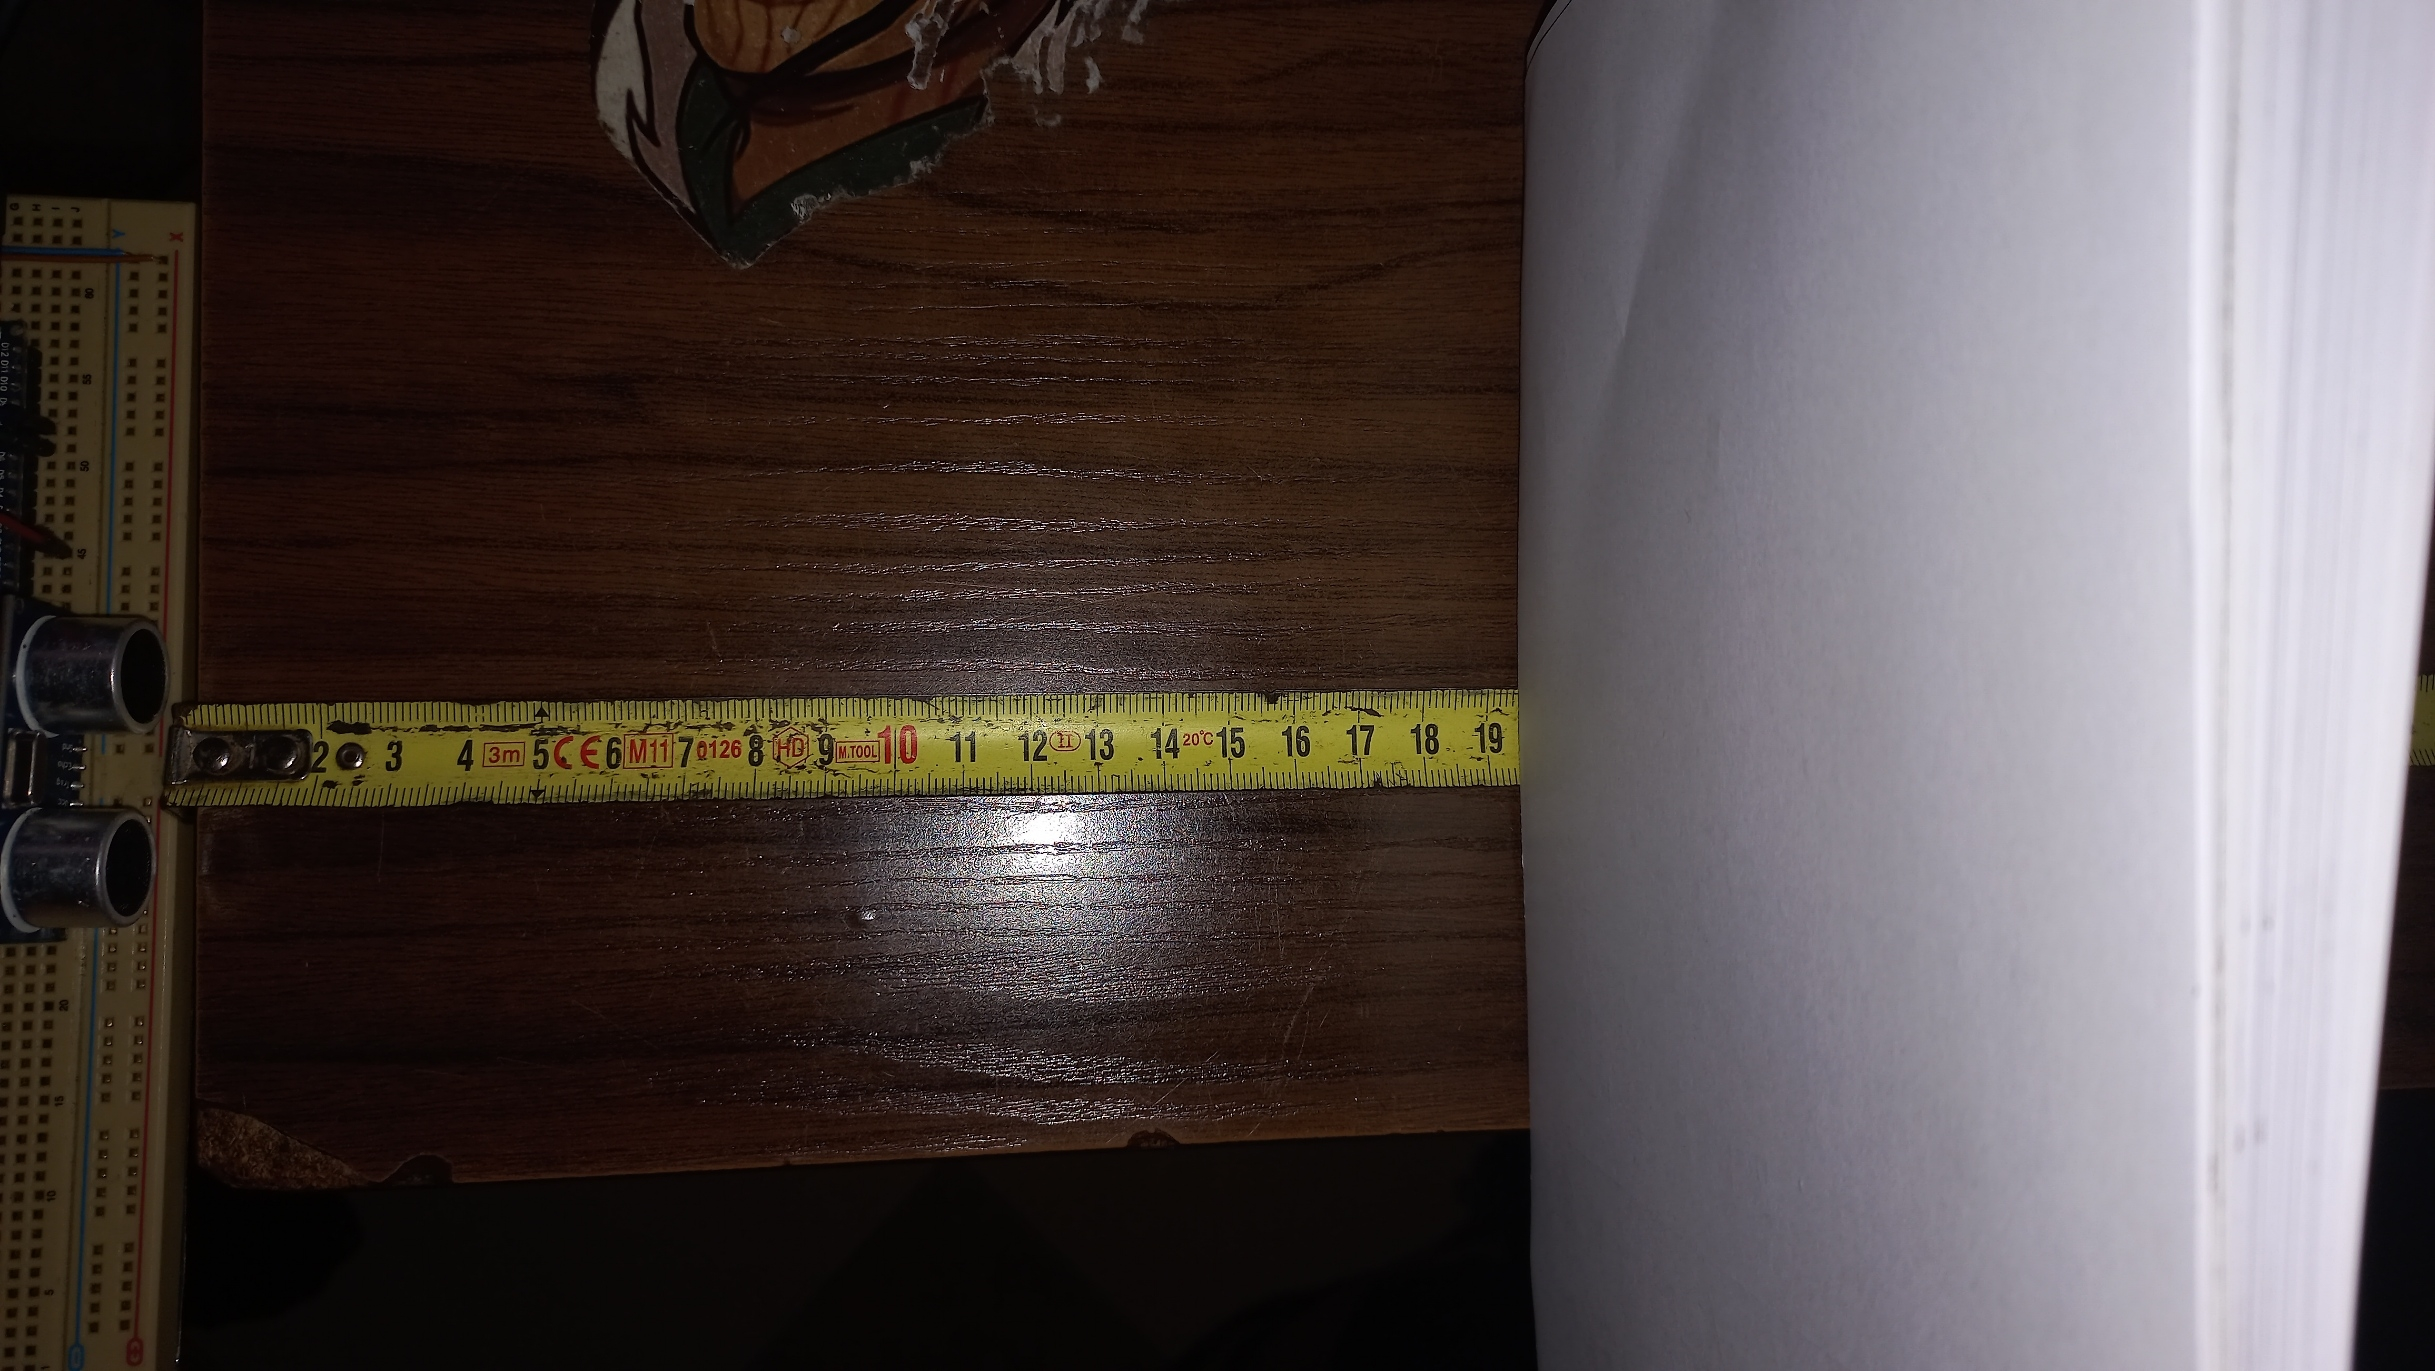
\includegraphics[width=\textwidth]{assets/HC-SR04/essais/19cm.jpg}
            \subcaption{Distance de 19cm}
        \end{subfigure}
        \\[8pt]
        \begin{subfigure}{\textwidth}
            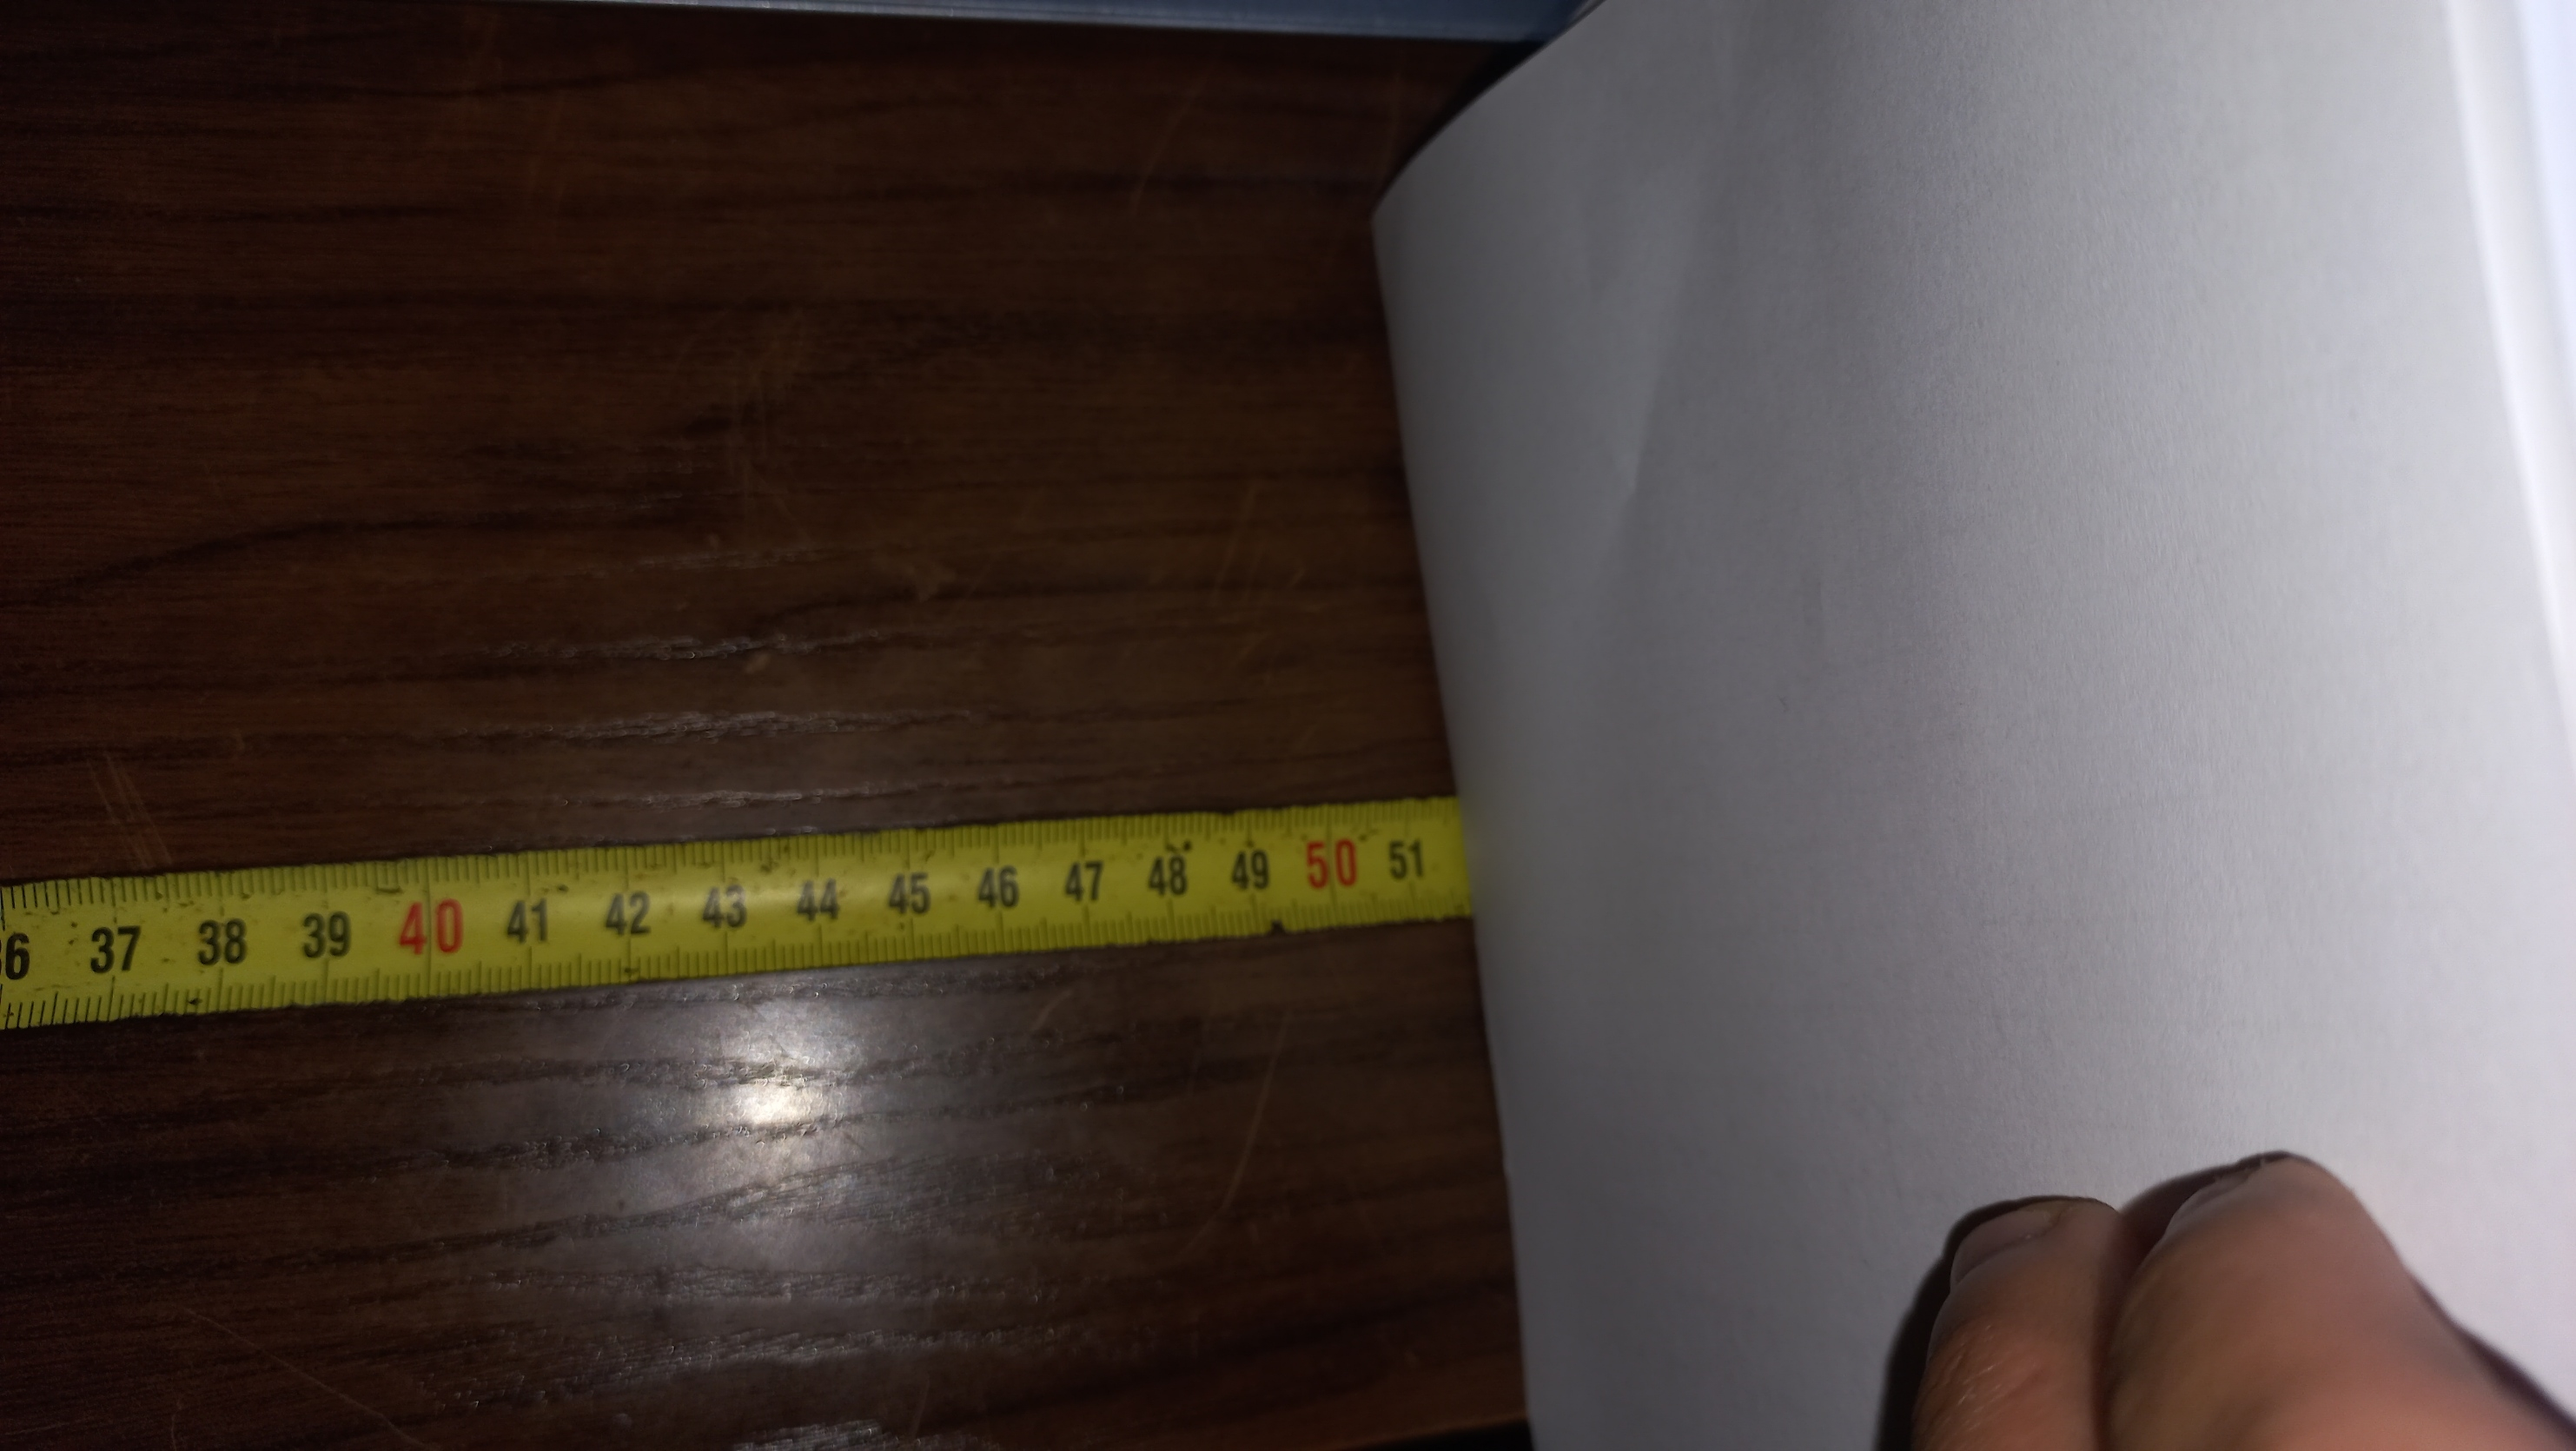
\includegraphics[width=\textwidth]{assets/HC-SR04/essais/52cm.jpg}
            \subcaption{Distance de 52cm}
        \end{subfigure}
    \end{subfigure}
    \hfill
    \begin{subfigure}[b]{.59\linewidth}
            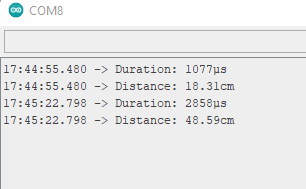
\includegraphics[width=\textwidth]{assets/HC-SR04/essais/resultat.png}
            \subcaption{Le résultat des deux essais}
    \end{subfigure}
    \caption{Essais pratique de HC-SR04}
\end{figure}

\FloatBarrier

Vous pouvez remarquer que la distance lue par le HC-SR04 n’est pas exactement la distance indiquée sur le ruban à mesurer. Cela se résume à deux raisons:
\begin{itemize}
    \item Nous avons peut-être mal aligné le capteur avec le ruban à mesurer, il y a donc une erreur de quelques millimètres.
    \item La vitesse du son dans l’air n’est pas constante, il y a des facteurs externes qui la modifient comme l’humidité et la température.
\end{itemize}

\begin{figure}
    \centering
    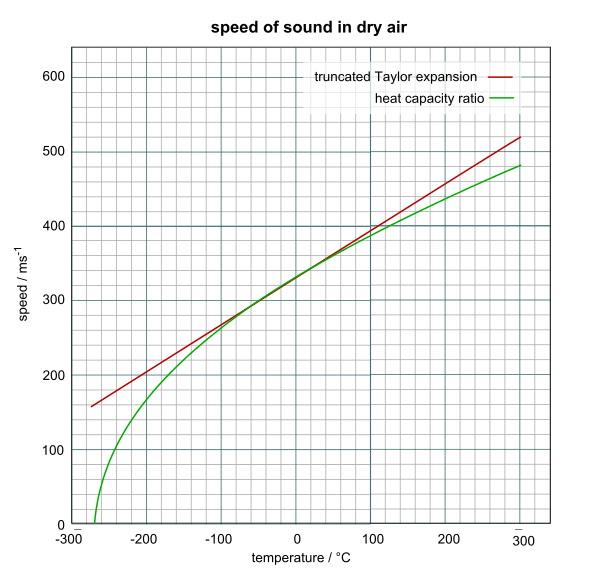
\includegraphics[width=.7\linewidth]{assets/Speed_of_sound_in_dry_air.png}
    \caption{Vitesse du son en fonction de la température}
\end{figure}

\FloatBarrier

Pour notre projet, nous n’avons pas besoin que notre mesure soit trop précise, quelques centimètres d’erreur ne feront pas problème.

\subsubsection{La vibration}

Avant de parler de vibration, il faut d’abord parler de sortie analogique en Arduino.

Malheureusement, Arduino ne propose pas des broches de sortie analogiques, mais elle offre une autre solution qui est \acrshort{PWM}.
En un mot, \acrshort{PWM} module la largeur de l’état HIGH dans un cycle de sortie, faisant le signal ressembler à un signal rectangulaire, ce qui fait moteurs et autres composants se comportent comme si le signal est une tension analogique changeante et changer leur vitesse de rotation.
\[v =  A \cdot \frac{T_{on}}{T} \]

Arduino offre une range de 0\dots 255 comme une sortie \acrshort{PWM}, où 
\begin{itemize}
    \item \(0 \rightarrow T_{on} = 0 \therefore v = 0\)
    \item \(255 \rightarrow T_{on} = T \therefore v = A = 5 \text{volts}\)
\end{itemize}

\begin{figure}[!htbp]
    \centering
    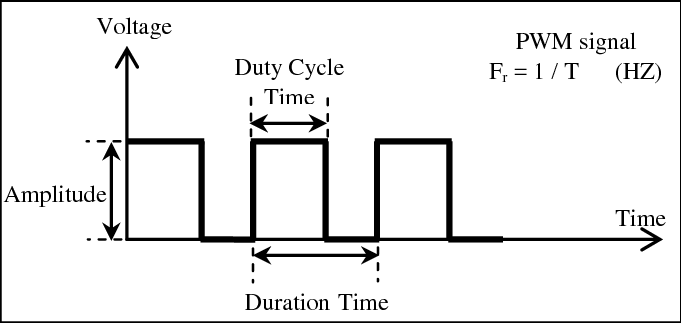
\includegraphics[width=.7\linewidth]{assets/PWM-signal-with-its-two-basic-time-periods.png}
    \caption{Exemple d'un signal \acrshort{PWM}}
\end{figure}

\FloatBarrier

Après de nombreux tests, nous avons constaté que 1m est la distance parfaite pour alarmer l’utilisateur, où l’intensité des vibrations augmente plus l’obstacle est proche. \\
Où la sortie \acrshort{PWM} passe de 50 pour des distances de 100cm à 255 pour toute distance inférieure à 2cm

\begin{figure}[!htbp]
    \centering
    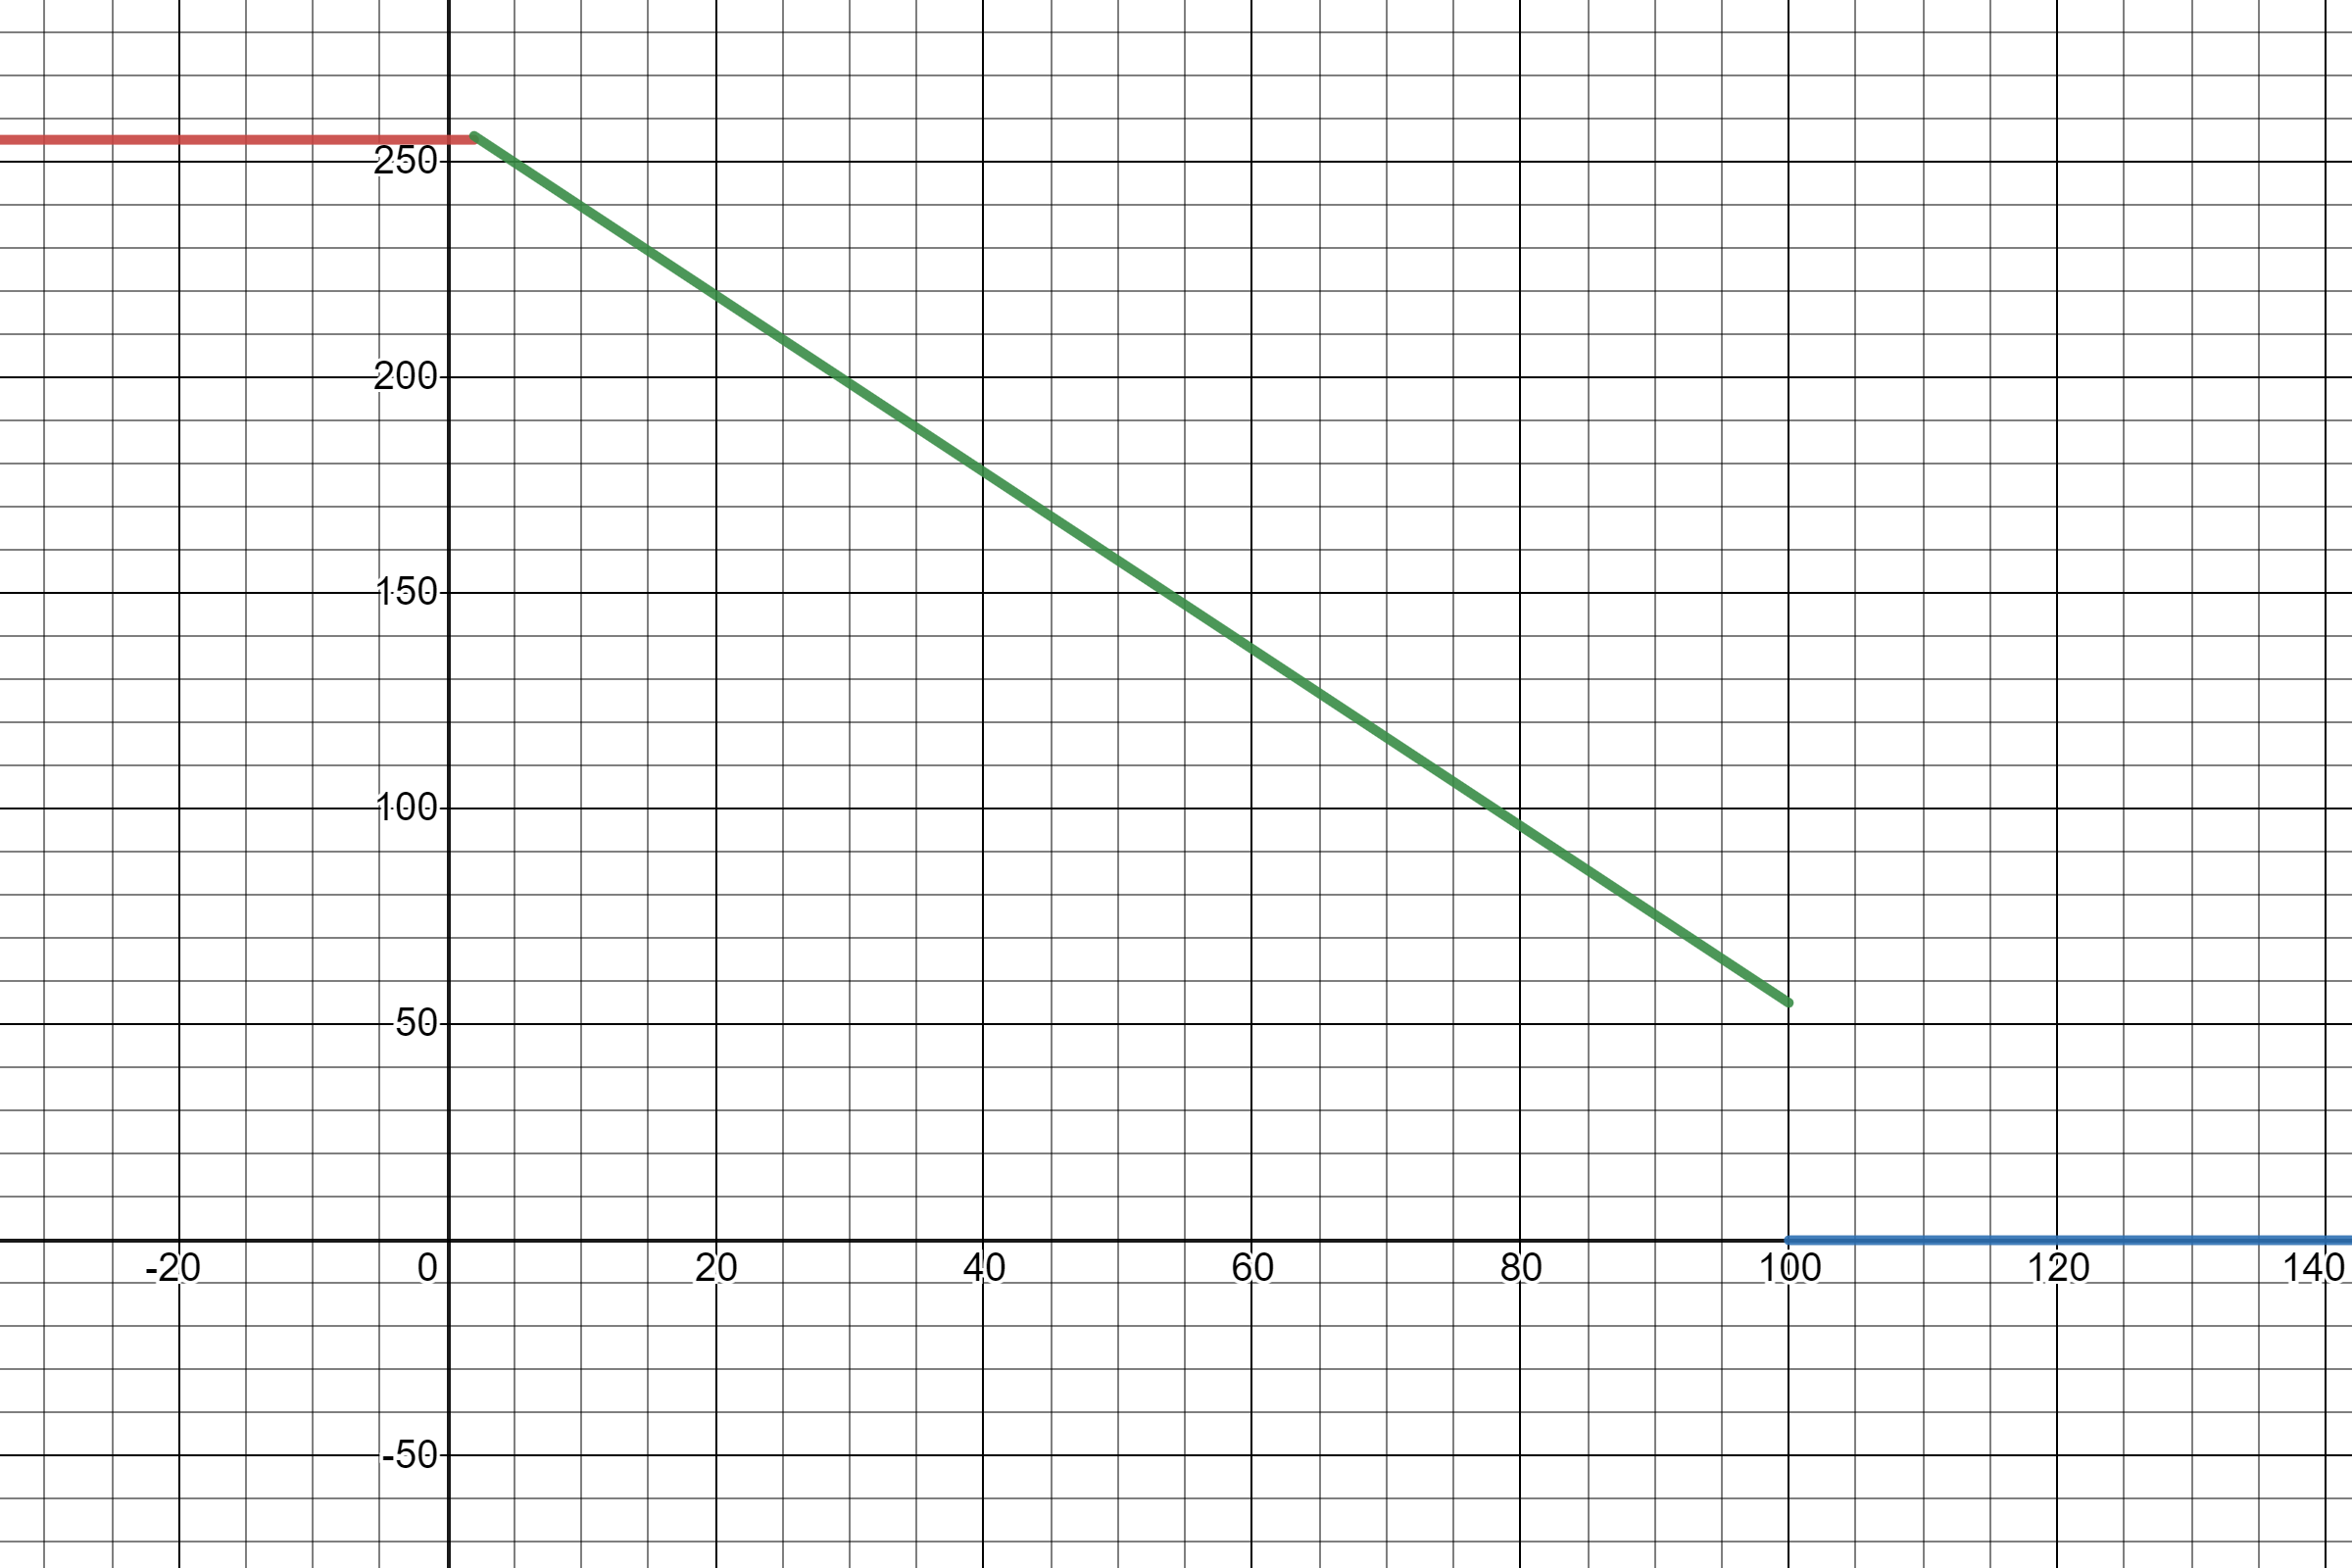
\includegraphics[width=.9\linewidth]{assets/HC-SR04/fonction de vibration.png}
    \caption{Sortie \acrshort{PWM} en fonction de la proximité d'obstacle}
\end{figure}

\FloatBarrier

\begin{figure}[!htbp]
    \centering
    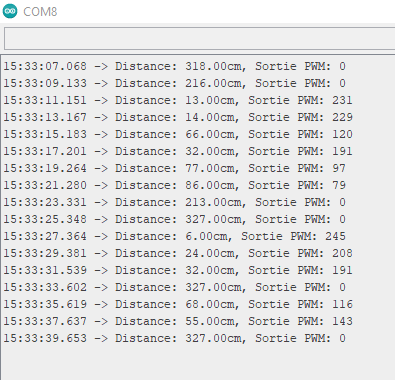
\includegraphics[width=.5\linewidth]{assets/HC-SR04/essais/PWM en fonction de distance.png}
    \caption{Essais de la sortie \acrshort{PWM} en fonction de la distance}
\end{figure}

\FloatBarrier

\begin{figure}[!htbp]
    \centering
    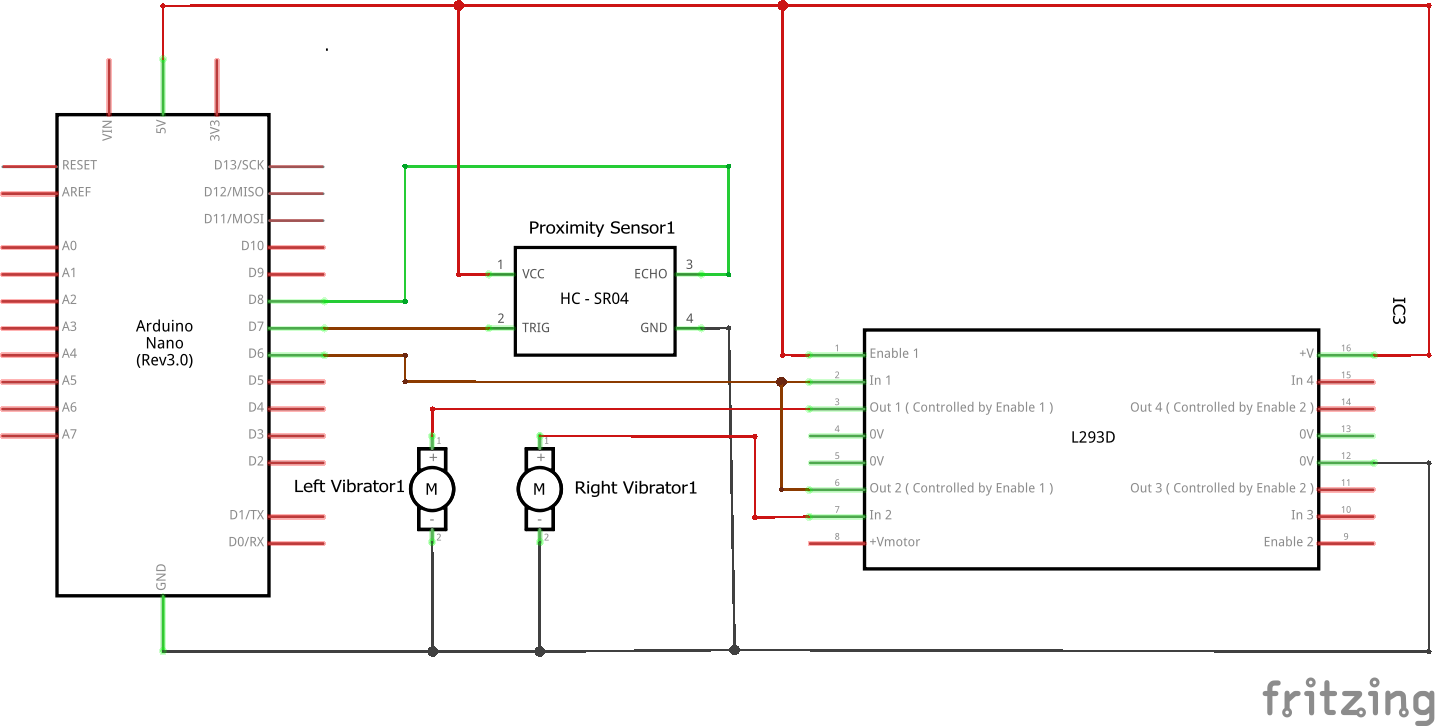
\includegraphics[width=\linewidth]{assets/HC-SR04/circuit avec vibration.png}
    \caption{Schéma avec la vibration de la connexion entre HC-SR04 avec l’arduino}
\end{figure}

\FloatBarrier

On a utiliser la broche 6 car elle supporte la sortie \acrfull{PWM}.

\subsubsection{Le problème avec l'approche actuelle}
Bien que notre code semble bien fonctionner pour le moment, il causera un problème indésirable en cours de route.

Le problème avec l’approche actuelle est qu’il est "blocking-code", ce qui signifie que pendant qu’il est en train d'exécuter, aucune autre tâche peut être faite... et nous vérifions les obstacles en continu, ce qui empêchent l’Arduino de faire autre chose que cela.

Le problème est causé par la fonction \verb|pulseIn| intégrée dans l’Arduino, alors qu’il calcule la durée d’une impulsion, il bloque le cycle d’exécution.

Nous allons créer notre propre système de mesure, en utilisant la fonction \verb|micros|.

\begin{figure}[!htbp]
    \centering
    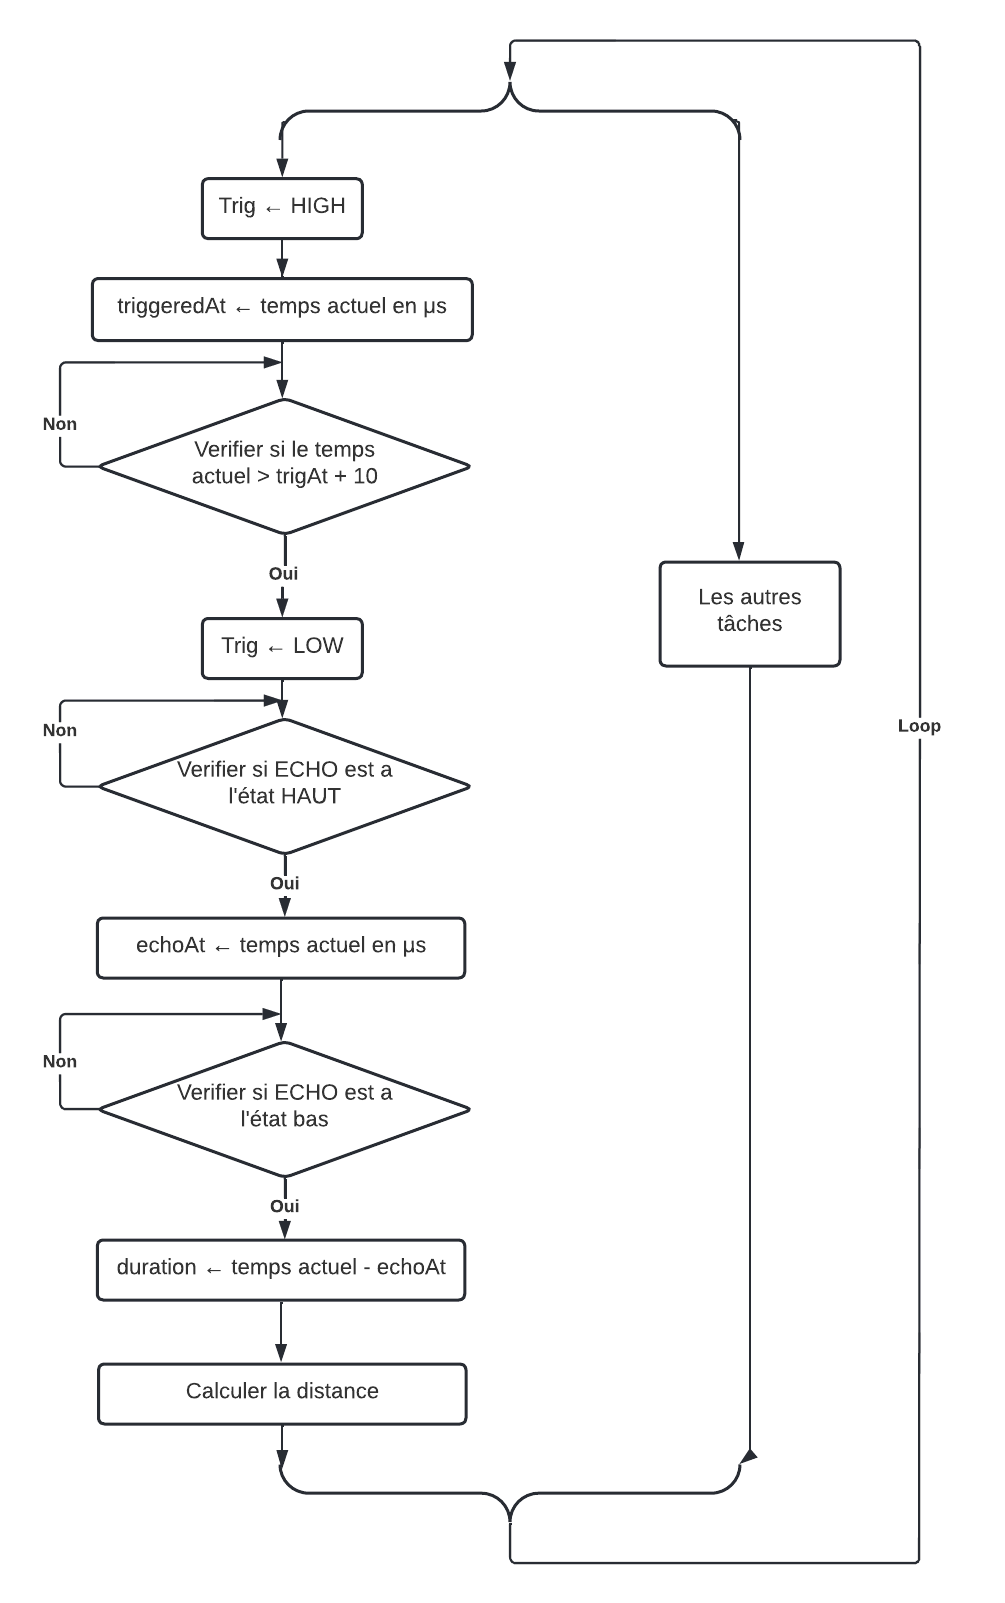
\includegraphics[height=.8\textheight]{assets/HC-SR04/our working principal.png}
    \caption{Logigramme de notre principe personnalisé de fonctionnement de HC-SR04}
\end{figure}

\FloatBarrier

Cette séquence fonctionne parfaitement, avec un seul autre problème : elle se bloque parfois.
Nous pouvons corriger cela en ajoutant un chien de garde (WatchDog) qui réinitialise les propriétés enregistrées (echoAt, trigAt) pour redémarrer le cycle et le débloquer. 

\begin{figure}[!htbp]
    \centering
    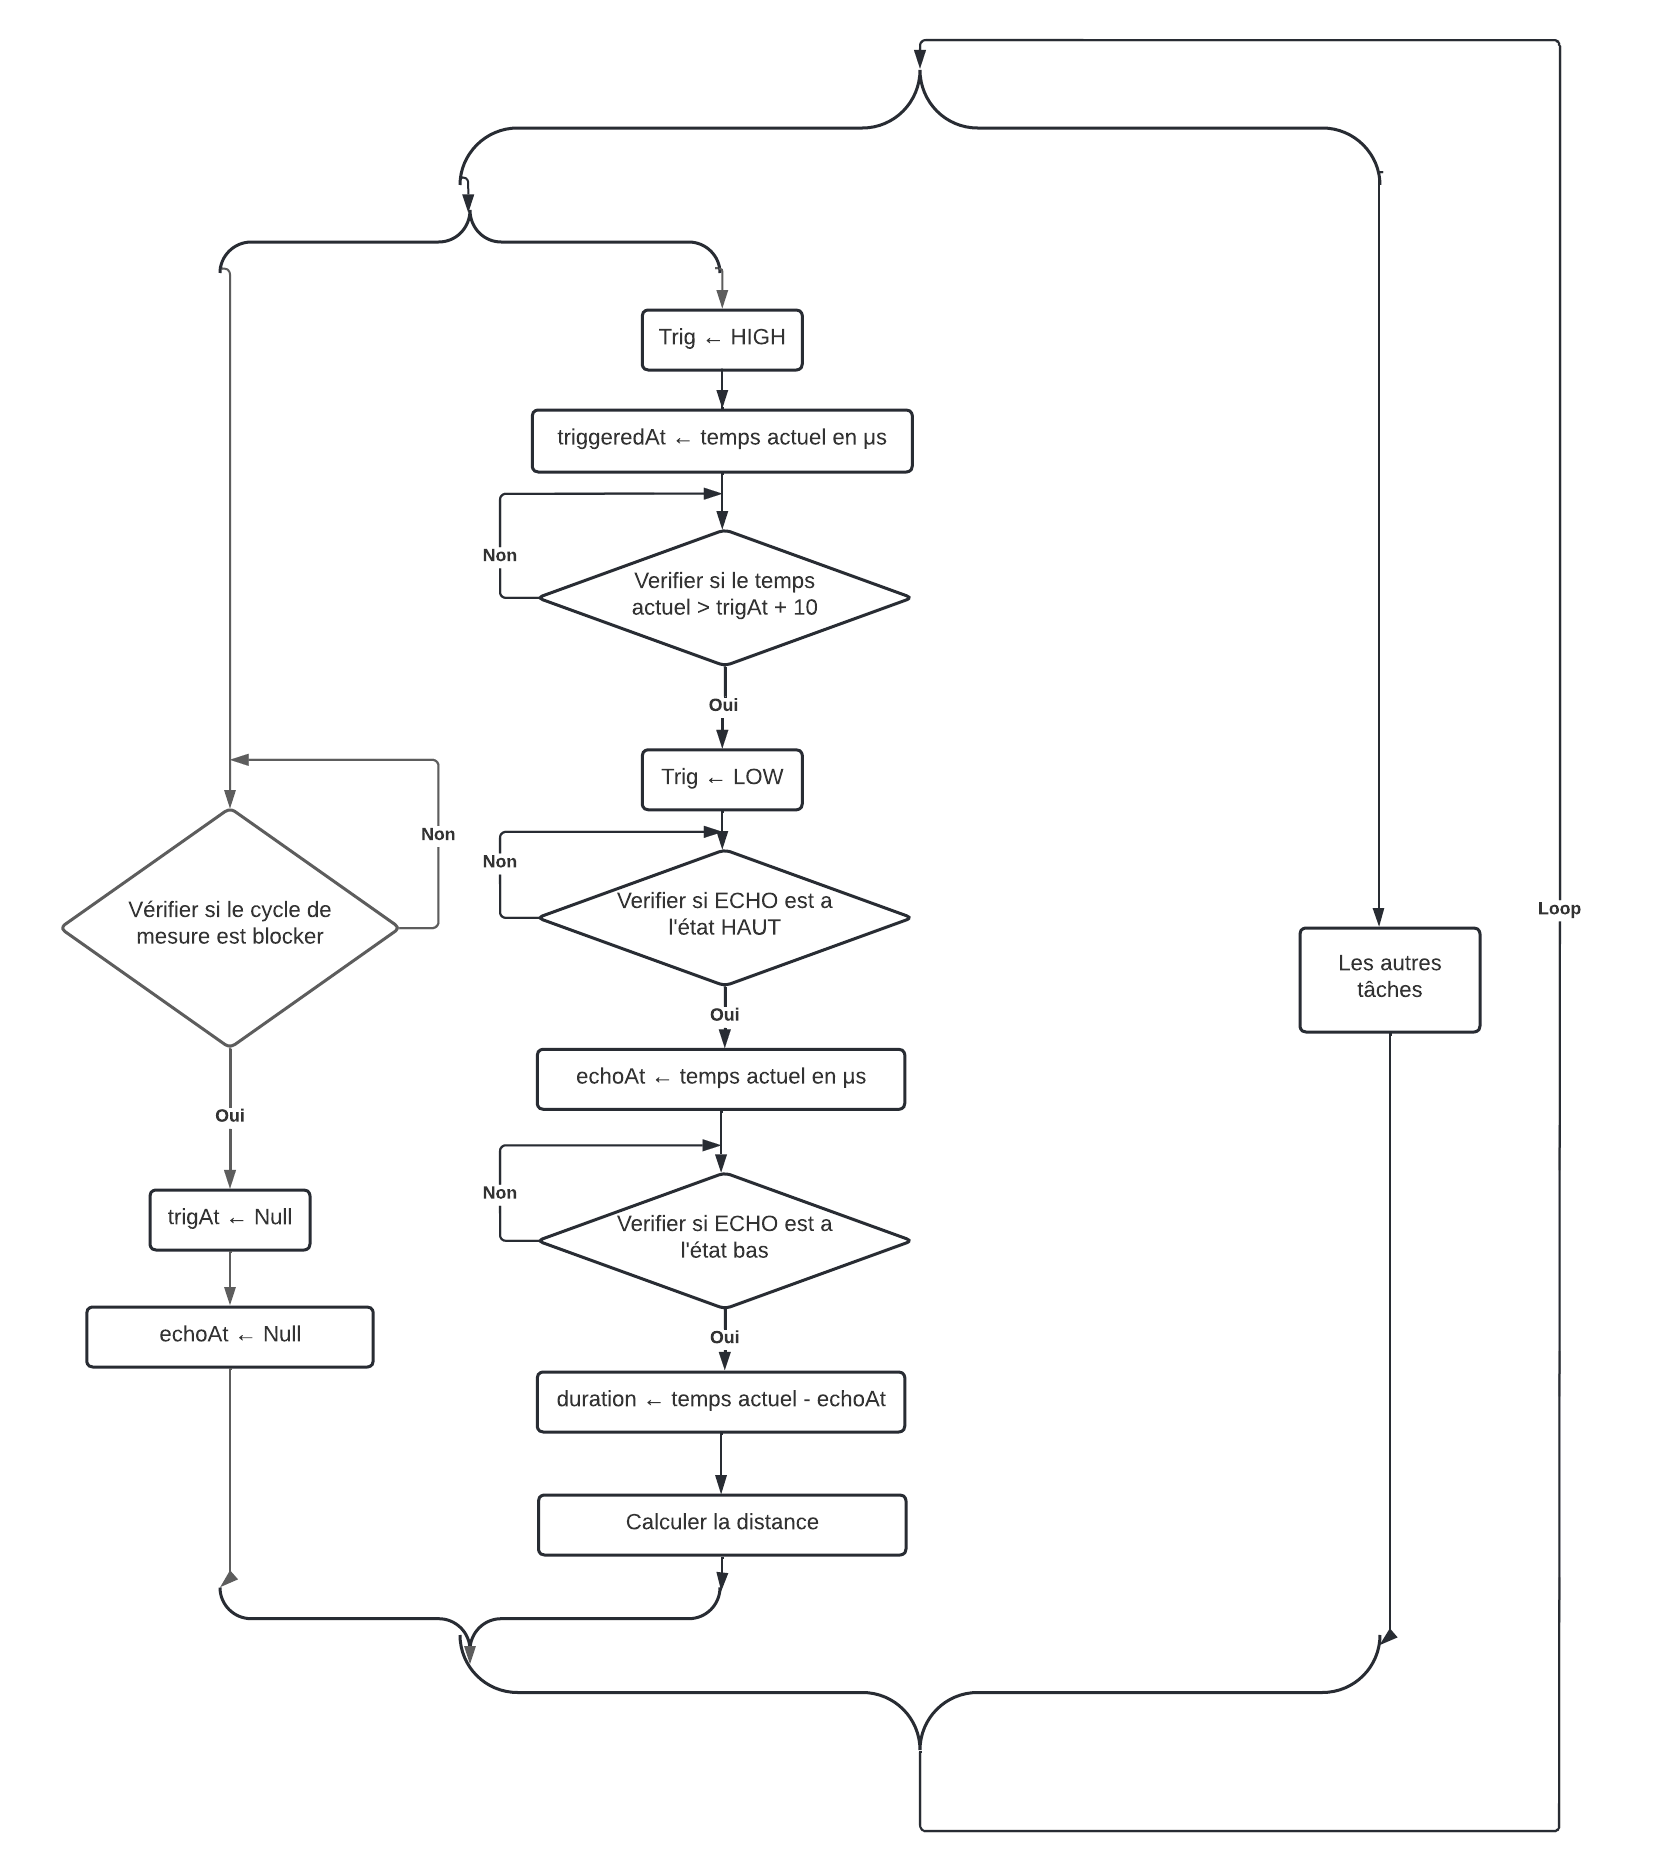
\includegraphics[height=.8\textheight, width=\linewidth]{assets/HC-SR04/our working principal with watchdog.png}
    \caption{Diagramme de notre principe personnalisé de fonctionnement de HC-SR04 avec le chien de garde}
\end{figure}

\FloatBarrier

\begin{code}
\begin{minted}[frame=single, framesep=3mm, linenos=true, xleftmargin=21pt, tabsize=4, fontsize=\small, breaklines]{cpp}
#include <Arduino.h>

#include "../Watchdog.cpp"
class HC_SR04 {

public:
    double threshold = 0;      // in cm
    unsigned long polling = 0; // in ms
    Watchdog watchdog;

private:
    int _echoPin;
    int _trigPin;
    void (*_onUpdate)(double);
    bool _isTriggering = false;
    unsigned long _triggeringStartedAt = 0;
    bool _isEchoing = false;
    unsigned long _echoingStartedAt = 0;

public:
    // echo, trig
    HC_SR04(
        int echo,
        int trig,
        void (*onUpdate)(double)
    ) {
        _echoPin = echo;
        _trigPin = trig;
        _onUpdate = onUpdate;
        pinMode(_trigPin, OUTPUT);
        pinMode(_echoPin, INPUT);
        digitalWrite(_trigPin, LOW);
        watchdog.barkAfter = 500;
    }

    void listen() {
        watchdog.watch();
        if (watchdog.bark)
        {
            reset();
            watchdog.feed();
        }
        if (_isEchoing)
        {
            if (digitalRead(_echoPin) && !_echoingStartedAt)
            {
                _echoingStartedAt = micros();
            }
            if (!digitalRead(_echoPin) && _echoingStartedAt)
            {
                unsigned long _duration = micros() - _echoingStartedAt;
                double _distance = _duration * 0.034 / 2;
                _isEchoing = false;
                _echoingStartedAt = 0;
                watchdog.feed();
                _onUpdate(_distance);
            }
        }
        else
        {
            if (!_isTriggering)
            {
                digitalWrite(_trigPin, HIGH);
                _triggeringStartedAt = micros();
                _isTriggering = true;
            }
            else if (_isTriggering && micros() >= _triggeringStartedAt + 10)
            {
                digitalWrite(_trigPin, LOW);
                _triggeringStartedAt = 0;
                _isTriggering = false;
                _isEchoing = true;
            }
        }
    }
    
    void reset() {
        _isTriggering = false;
        _triggeringStartedAt = 0;
        _isEchoing = false;
        _echoingStartedAt = 0;
    }
};
\end{minted}
\caption{HC-SR04}
\end{code}

\begin{code}
\begin{minted}[frame=single, framesep=3mm, linenos=true, xleftmargin=21pt, tabsize=4, fontsize=\small, breaklines]{cpp}
class Watchdog {
public:
    unsigned long long fedAt = 0;
    unsigned long long barkAfter = 1000;
    bool bark = false;

    Watchdog() {
        fedAt = millis();
    }

    void watch() {
        bark = millis() > (fedAt + barkAfter);
    }

    void feed() {
        fedAt = millis();
    }
};
\end{minted}
\caption{WatchDog}
\end{code}

\begin{code}
\begin{minted}[frame=single, framesep=3mm, linenos=true, xleftmargin=21pt, tabsize=4, fontsize=\small, breaklines]{cpp}
namespace ProximityVibrator {
    const int _VibratorPort = 5;

    const int MIN_VIBRATION_VAL = 50;
    const int MAX_VIBRATION_VAL = 255;

    const int SENSOR_THRESHOLD = 100;

    void onUpdate(double distance) {
        int _val = max(MIN_VIBRATION_VAL + (SENSOR_THRESHOLD - distance) * (MAX_VIBRATION_VAL - MIN_VIBRATION_VAL) / (SENSOR_THRESHOLD - 2), 0);
        if (_val < MIN_VIBRATION_VAL)
            _val = 0;
        analogWrite(_VibratorPort, _val);
    }

    HC_SR04 sensor(8, 7, onUpdate); // Echo, Trig, onUpdate

    void setup() {
        pinMode(_VibratorPort, OUTPUT);
        sensor.threshold = SENSOR_THRESHOLD;
    }

    void loop() {
        sensor.listen();
    }
}
\end{minted}
\caption{Vibreur}
\end{code}

\subsubsection{Conclusion}

Et avec cela, nous avons exécuté avec succès la tâche d’avertir l’utilisateur sur les obstacles devant lui, sans perturber d’autres tâches

\subsection{La navigation}
Comme discuté avant, nous utiliserons les différents services Google afin de trouver les informations à propos les différents endroits.

\subsubsection{Les endroits à proximité}

\begin{figure}[!htbp]
    \centering
    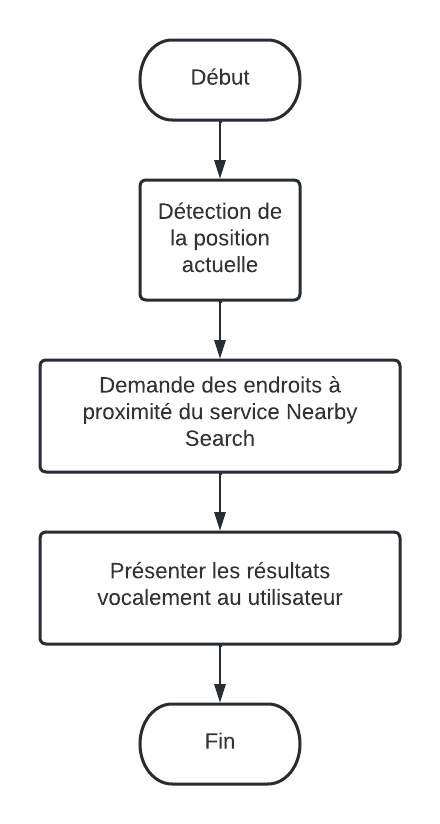
\includegraphics[width=.5\linewidth]{assets/app/explore/simplified logigramme.png}
    \caption{Diagramme simplifié de la recherche des endroits à proximité}
\end{figure}

\FloatBarrier
  
\begin{code}
\begin{minted}[frame=single, framesep=3mm, linenos=true, xleftmargin=21pt, tabsize=4, fontsize=\small, breaklines]{dart}
Future<List<SearchResult>?> searchNearbyPlaces(String? type) async {
    var location = Provider.of<LocationService>(GlobalContextService.navigatorKey
    .currentContext!, listen: false);
    var currentLocation = await location.updateCurrentLocation();

    if (currentLocation == null) {
      return null;
    }

    try {
      var result = await googlePlace.search.getNearBySearch(
        Location(
          lat: currentLocation.latitude,
          lng: currentLocation.longitude,
        ),
        1000,
        type: type,
      );
      return result?.results;
    } catch (exception) {
      inspect(exception);
      return null;
    }
}
\end{minted}
\caption{Search for nearby places}
\end{code}

\begin{figure}[!htbp]
    \centering
    \begin{subfigure}{.45\linewidth}
        \centering
         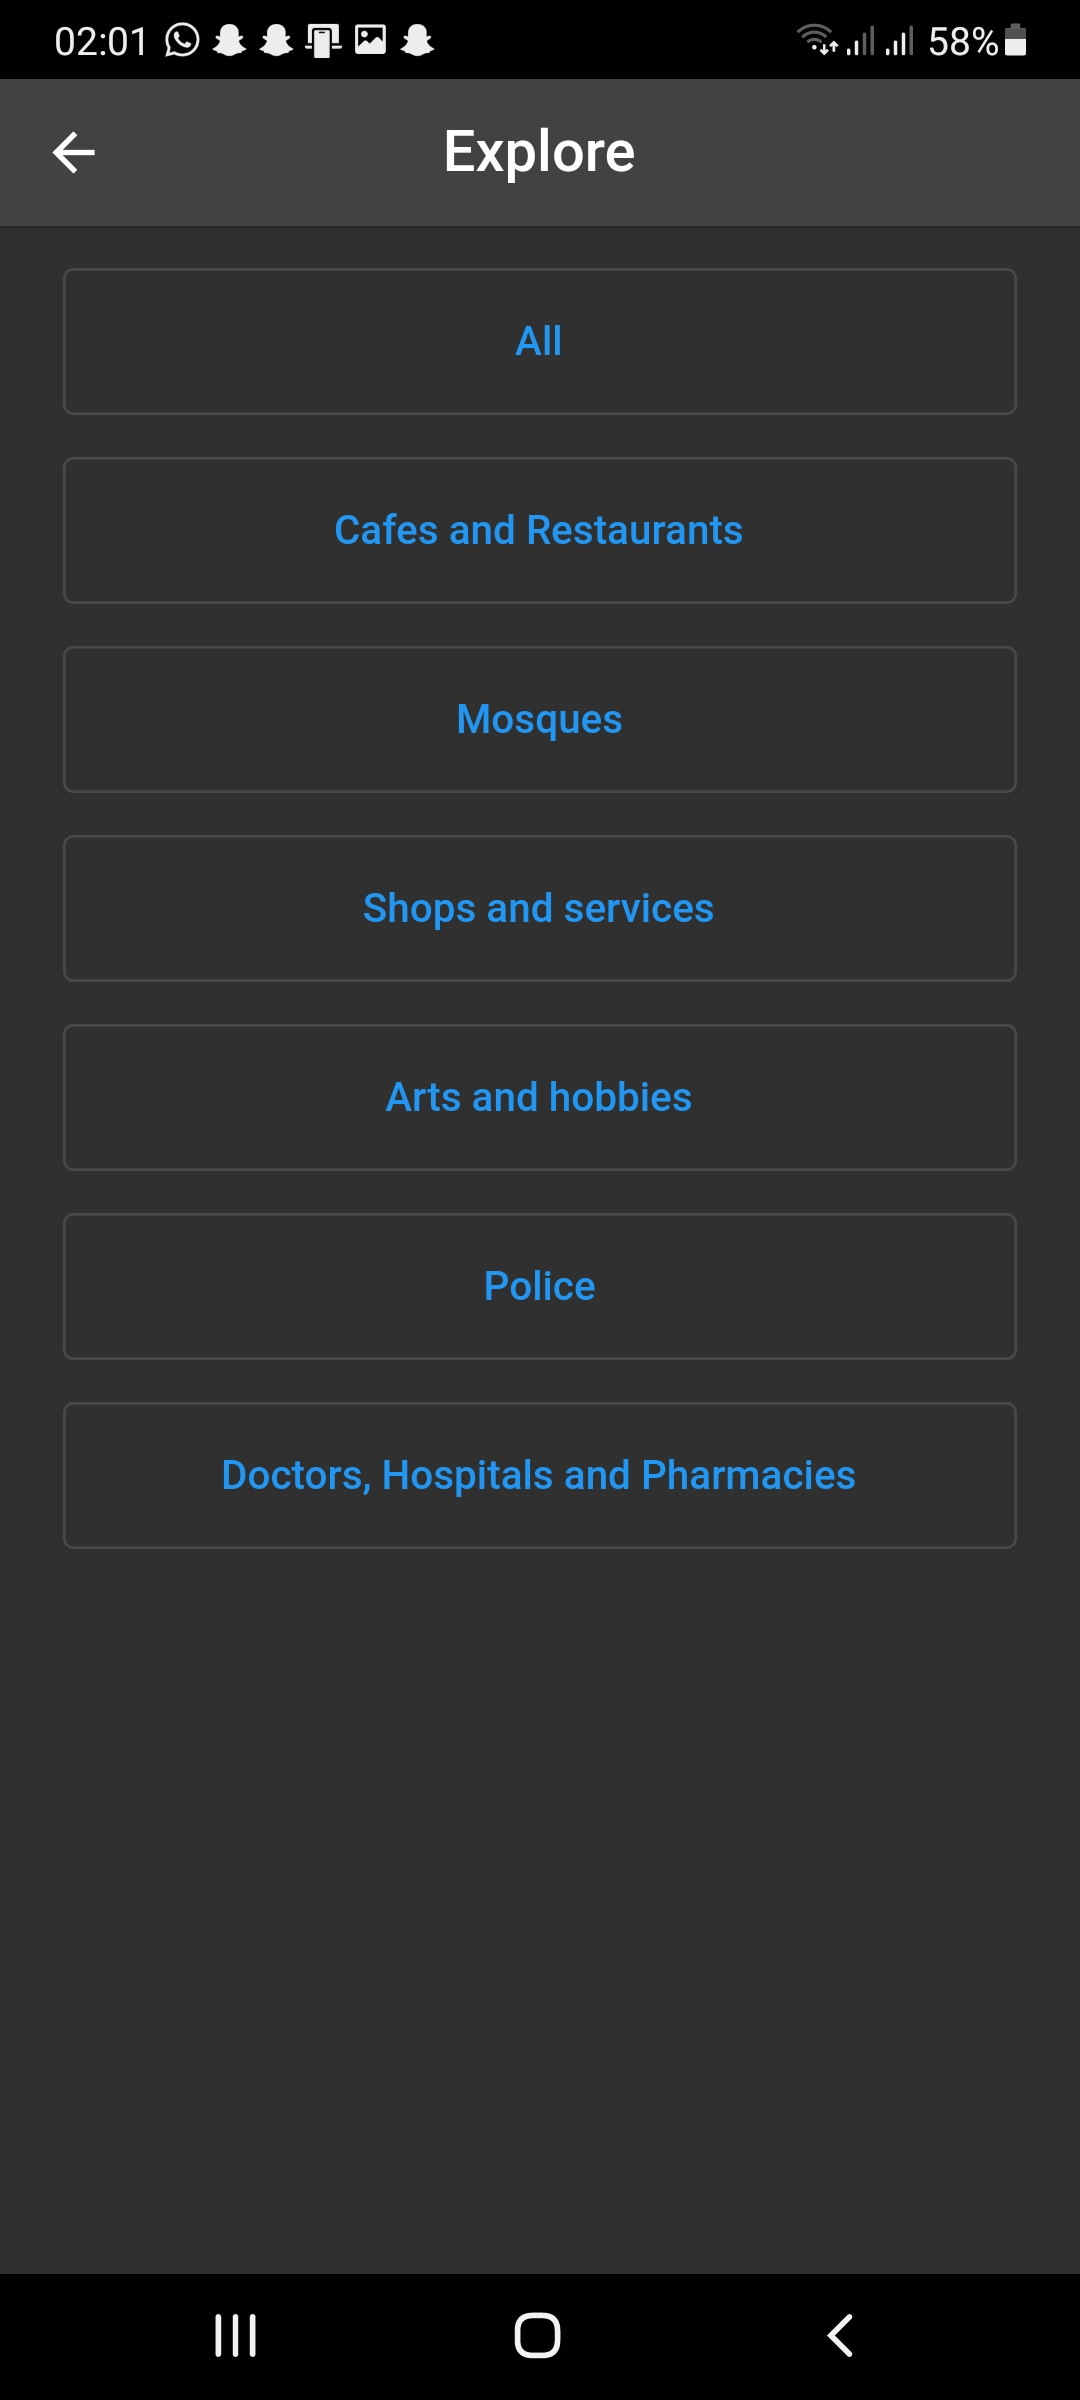
\includegraphics[width=\textwidth]{assets/app/explore/select type.jpg}
         \caption{Sélection du type des endroits voulus}
    \end{subfigure} 
    \hfill
    \begin{subfigure}{.45\linewidth}
        \centering
         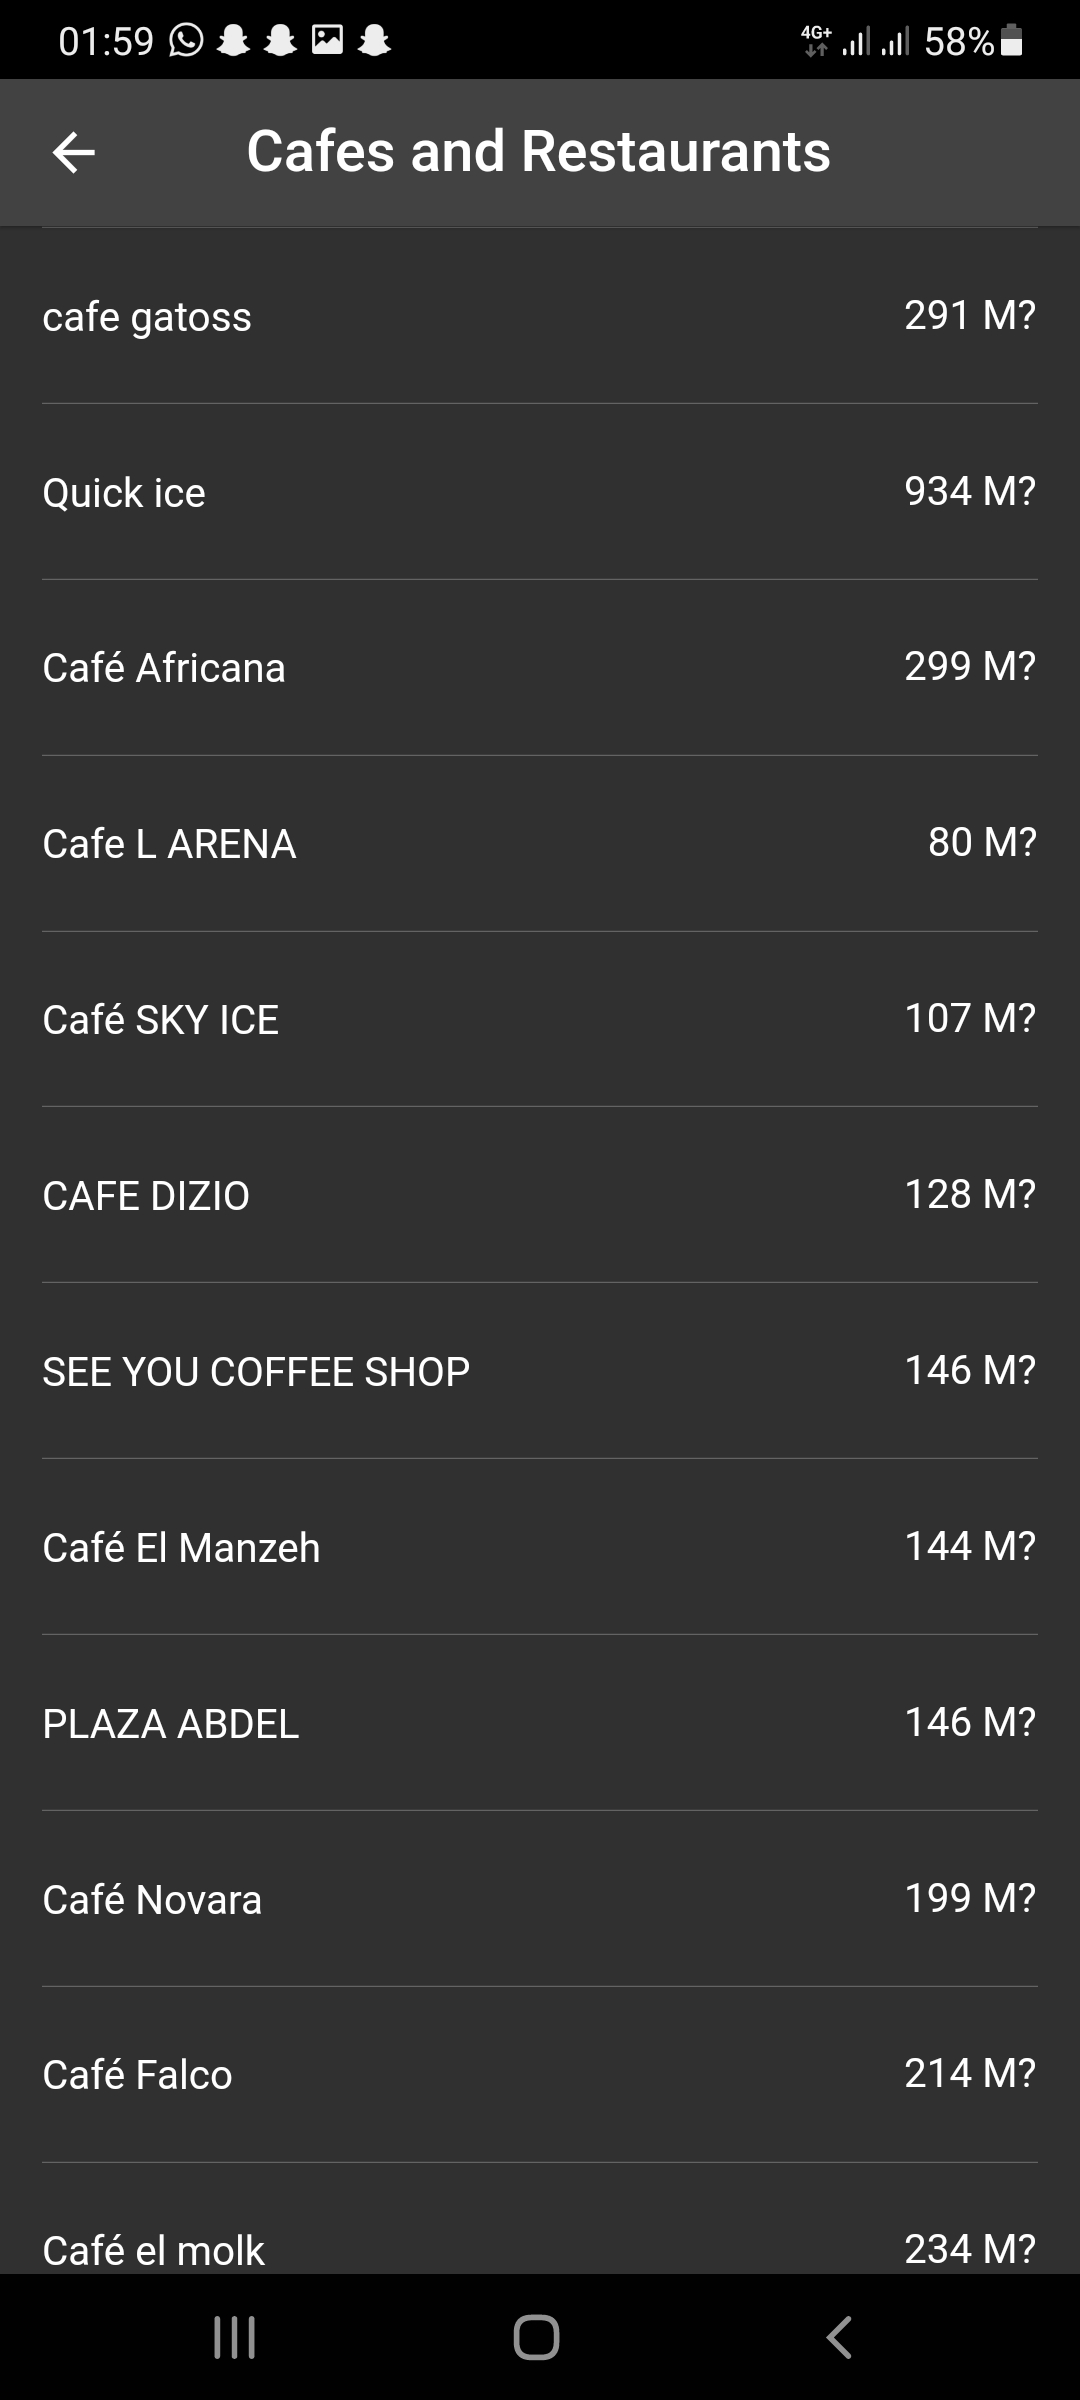
\includegraphics[width=\textwidth]{assets/app/explore/result.jpg}
         \caption{Résultats de recherche}
    \end{subfigure}
    \caption{Recherche des endroits à proximité}
\end{figure}

\FloatBarrier

\subsubsection{Recherche d'un endroit voulu}

\begin{figure}[!htbp]
    \centering
    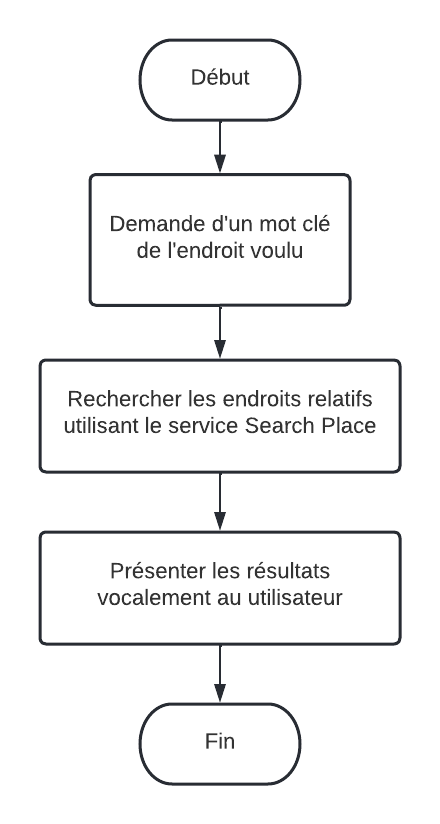
\includegraphics[width=.5\linewidth]{assets/app/search/diagramme.png}
    \caption{Diagramme simplifié de la recherche d'un endroit voulu}
\end{figure}

\FloatBarrier
  
\begin{code}
\begin{minted}[frame=single, framesep=3mm, linenos=true, xleftmargin=21pt, tabsize=4, fontsize=\small, breaklines]{dart}
void onSearch() async {
    setState(() {
      _places = [];
      isLoading = true;
    });

    var result = await googlePlace.search.getTextSearch(
      _inputController.value.text,
      language: "fr",
    );

    if (result == null || result.results == null) return;

    for (var element in result.results!) {
      _places.add(
        Place(
          info: DetailsResult(
            name: element.name,
            placeId: element.placeId,
            geometry: element.geometry,
          ),
        ),
      );

      setState(() {
        isLoading = false;
      });
    }

    for (var i = 0; i < _places.length; i++) {
      var place = _places.elementAt(i);
      _places[i].directions.walking = await Helpers.getDirections(destination: place);
      setState(() {});
    }
}
\end{minted}
\caption{Recherche d'un endroit voulu}
\end{code}

\begin{figure}[!htbp]
    \centering
    \begin{subfigure}{.3\linewidth}
        \centering
         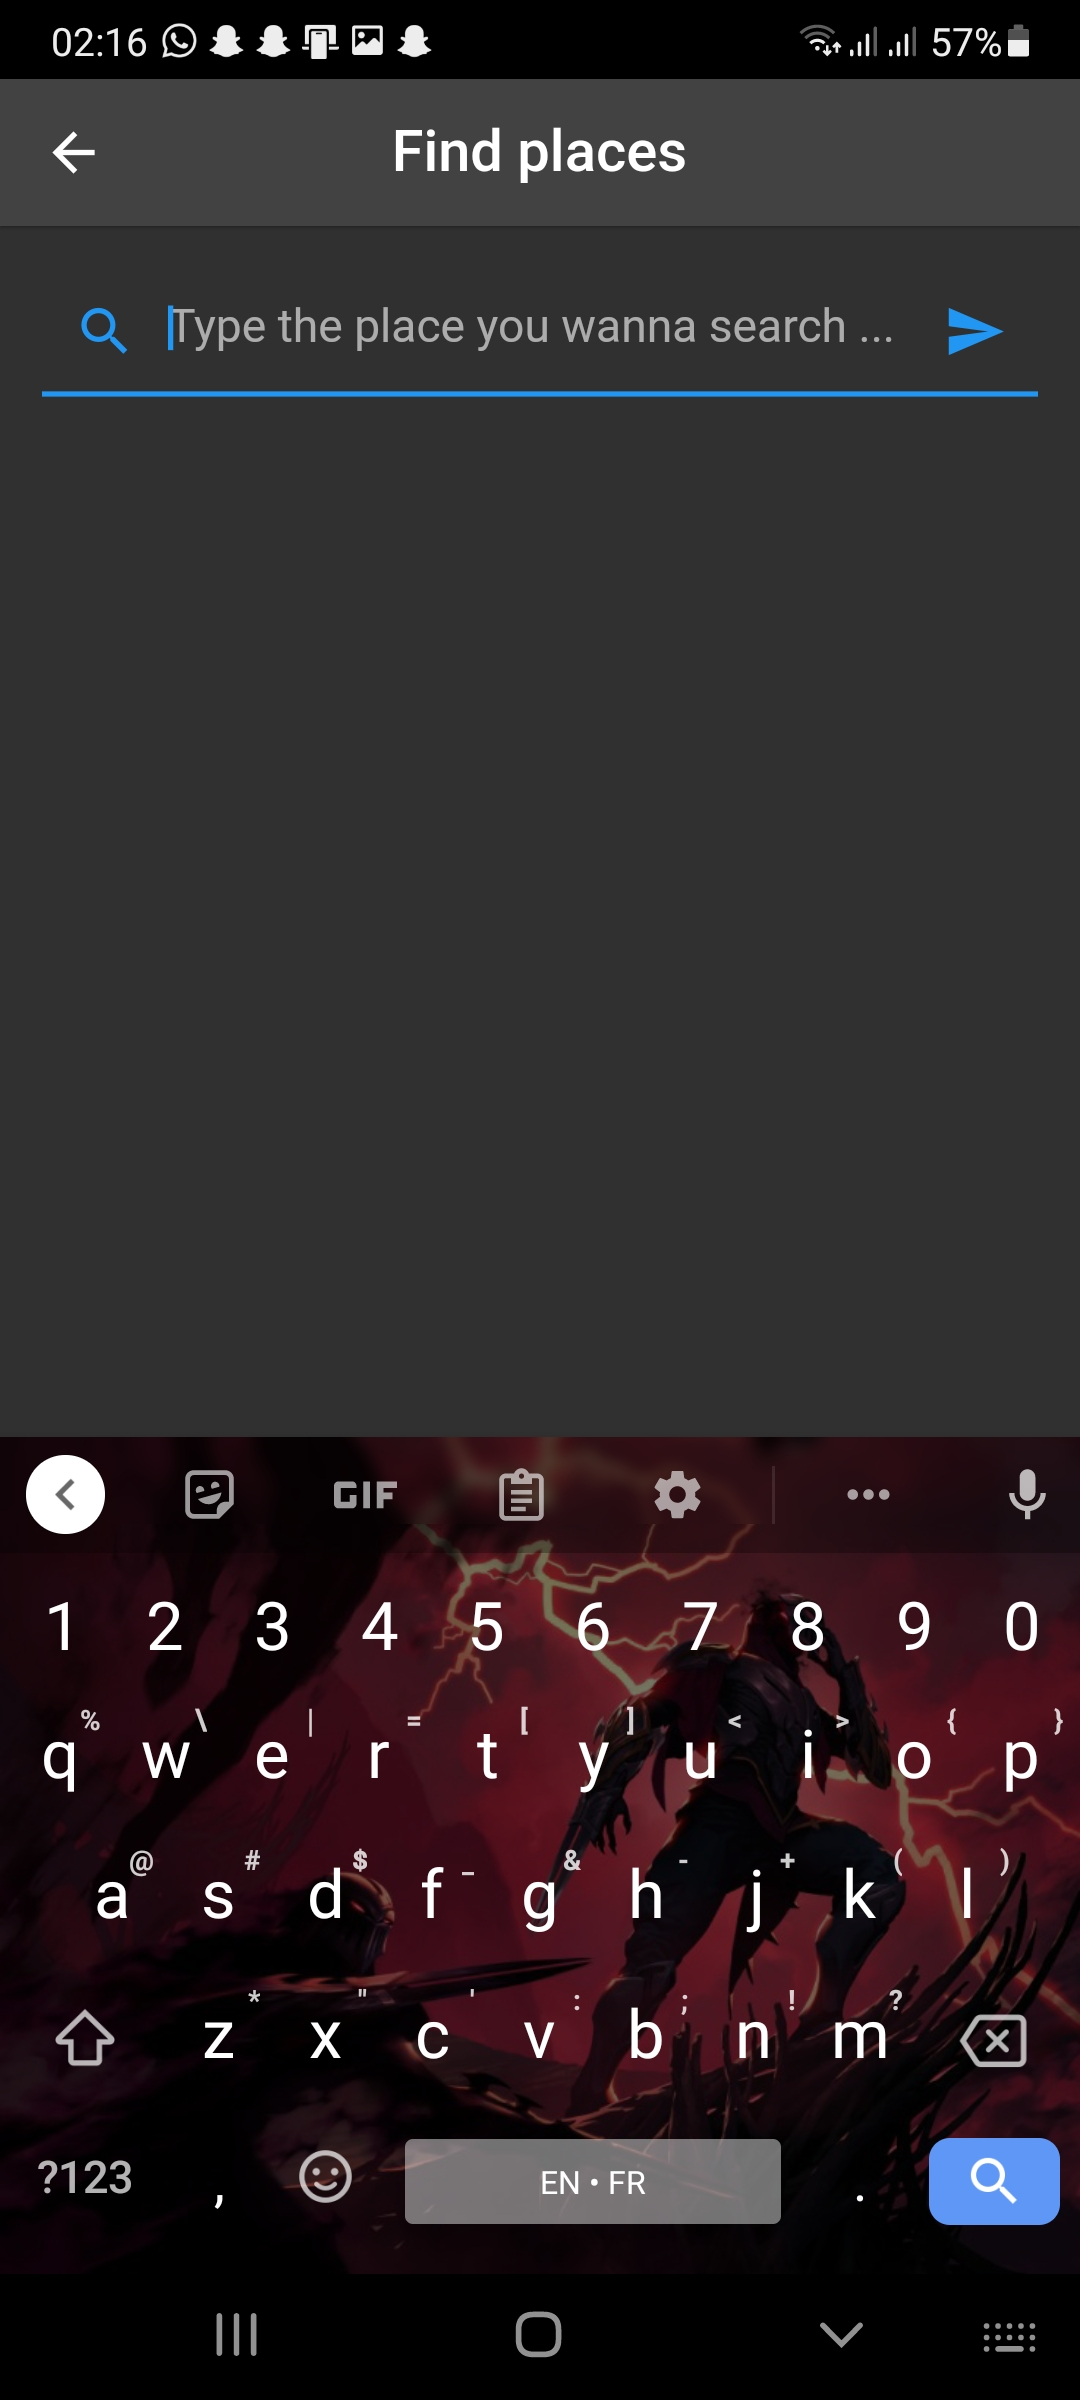
\includegraphics[width=\textwidth]{assets/app/search/search.jpg}
         \caption{Barre de recherche}
    \end{subfigure} 
    \hfill
    \begin{subfigure}{.3\linewidth}
        \centering
         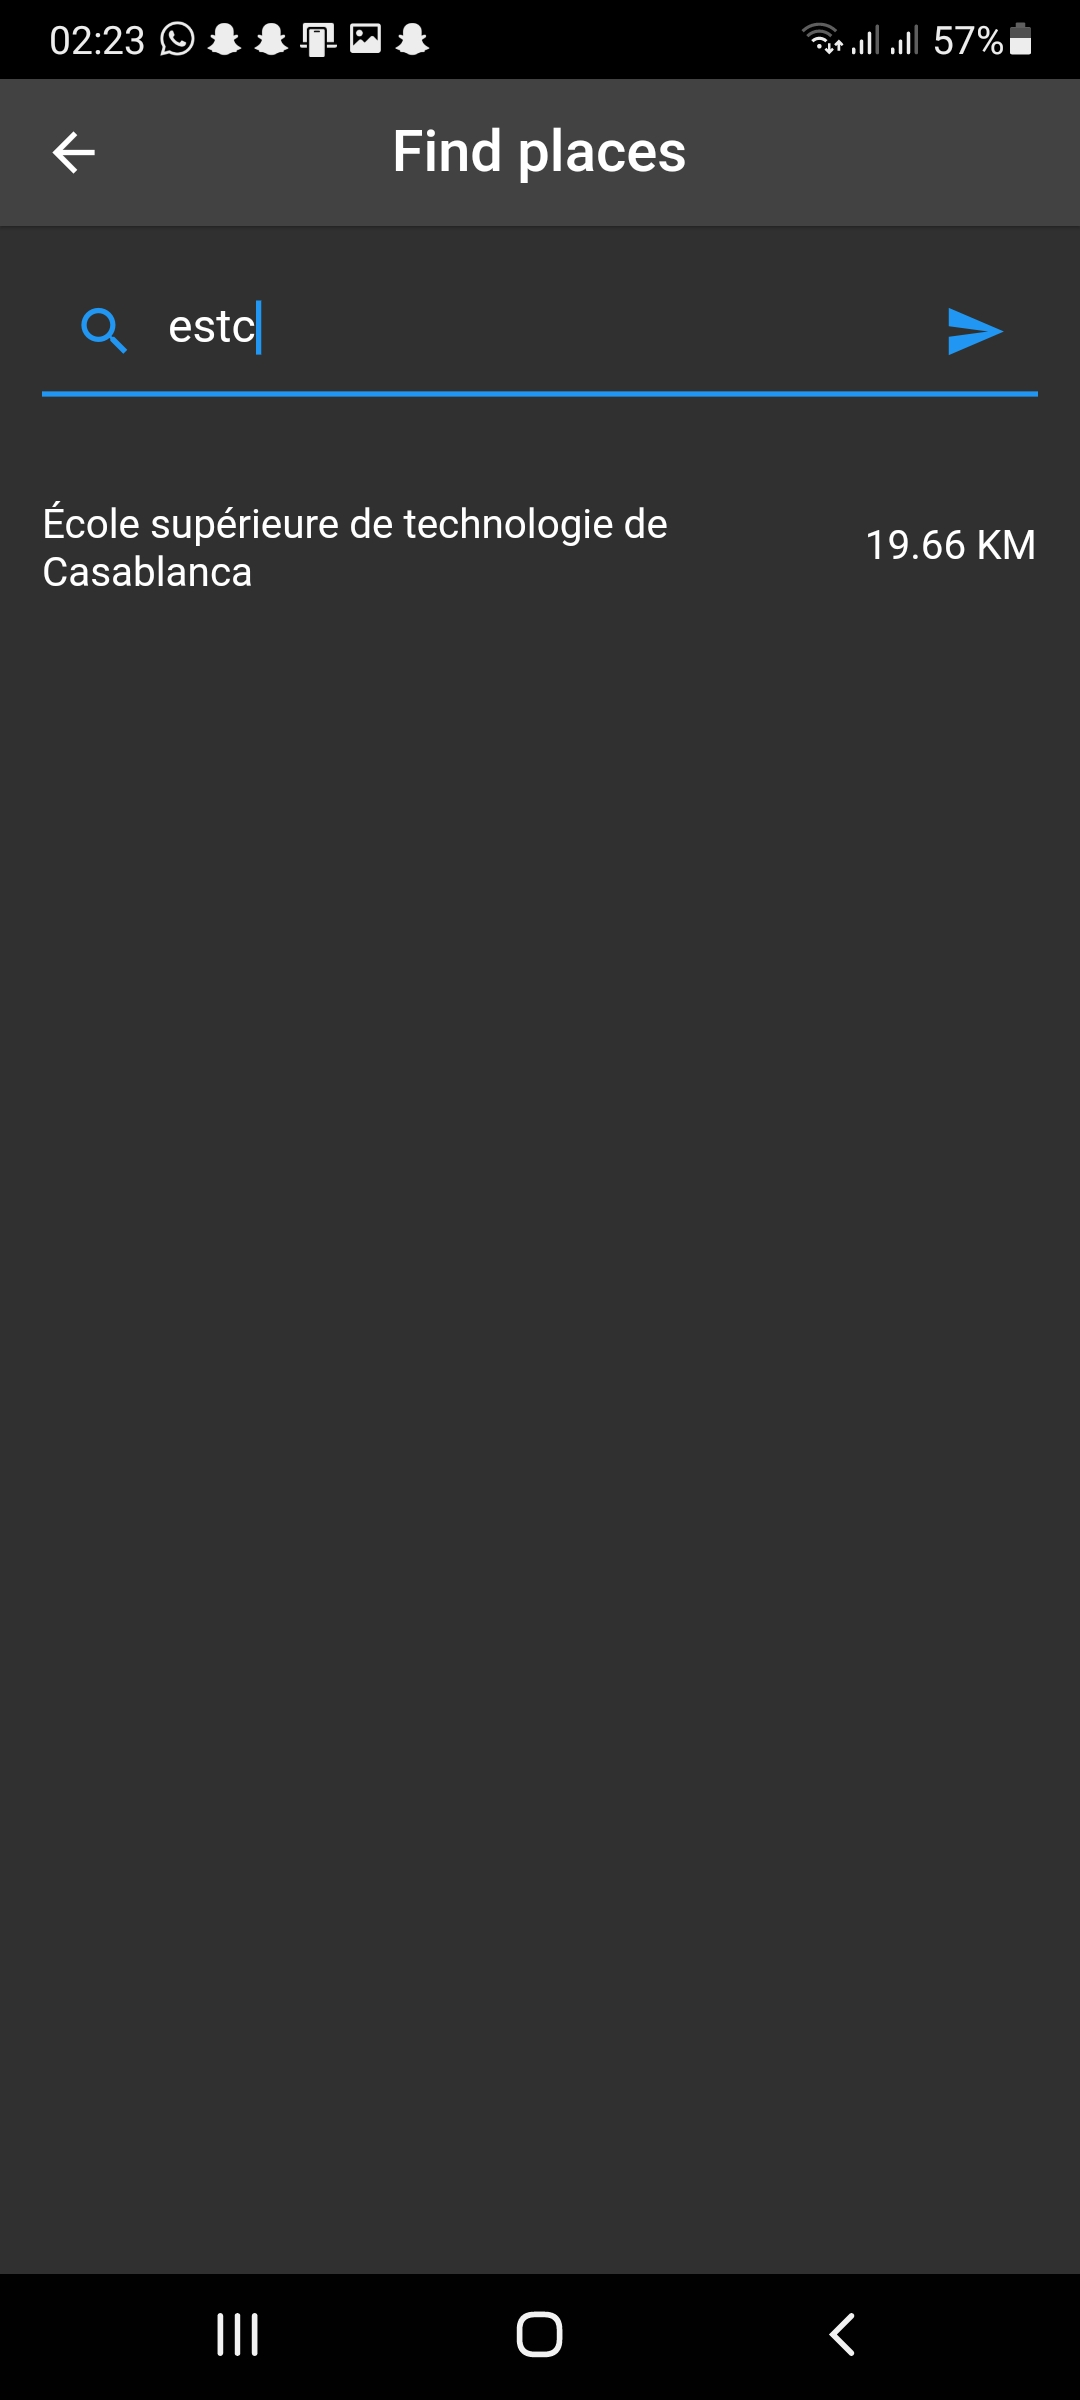
\includegraphics[width=\textwidth]{assets/app/search/result.jpg}
         \caption{Résultats de recherche}
    \end{subfigure}
    \hfill
    \begin{subfigure}{.3\linewidth}
        \centering
         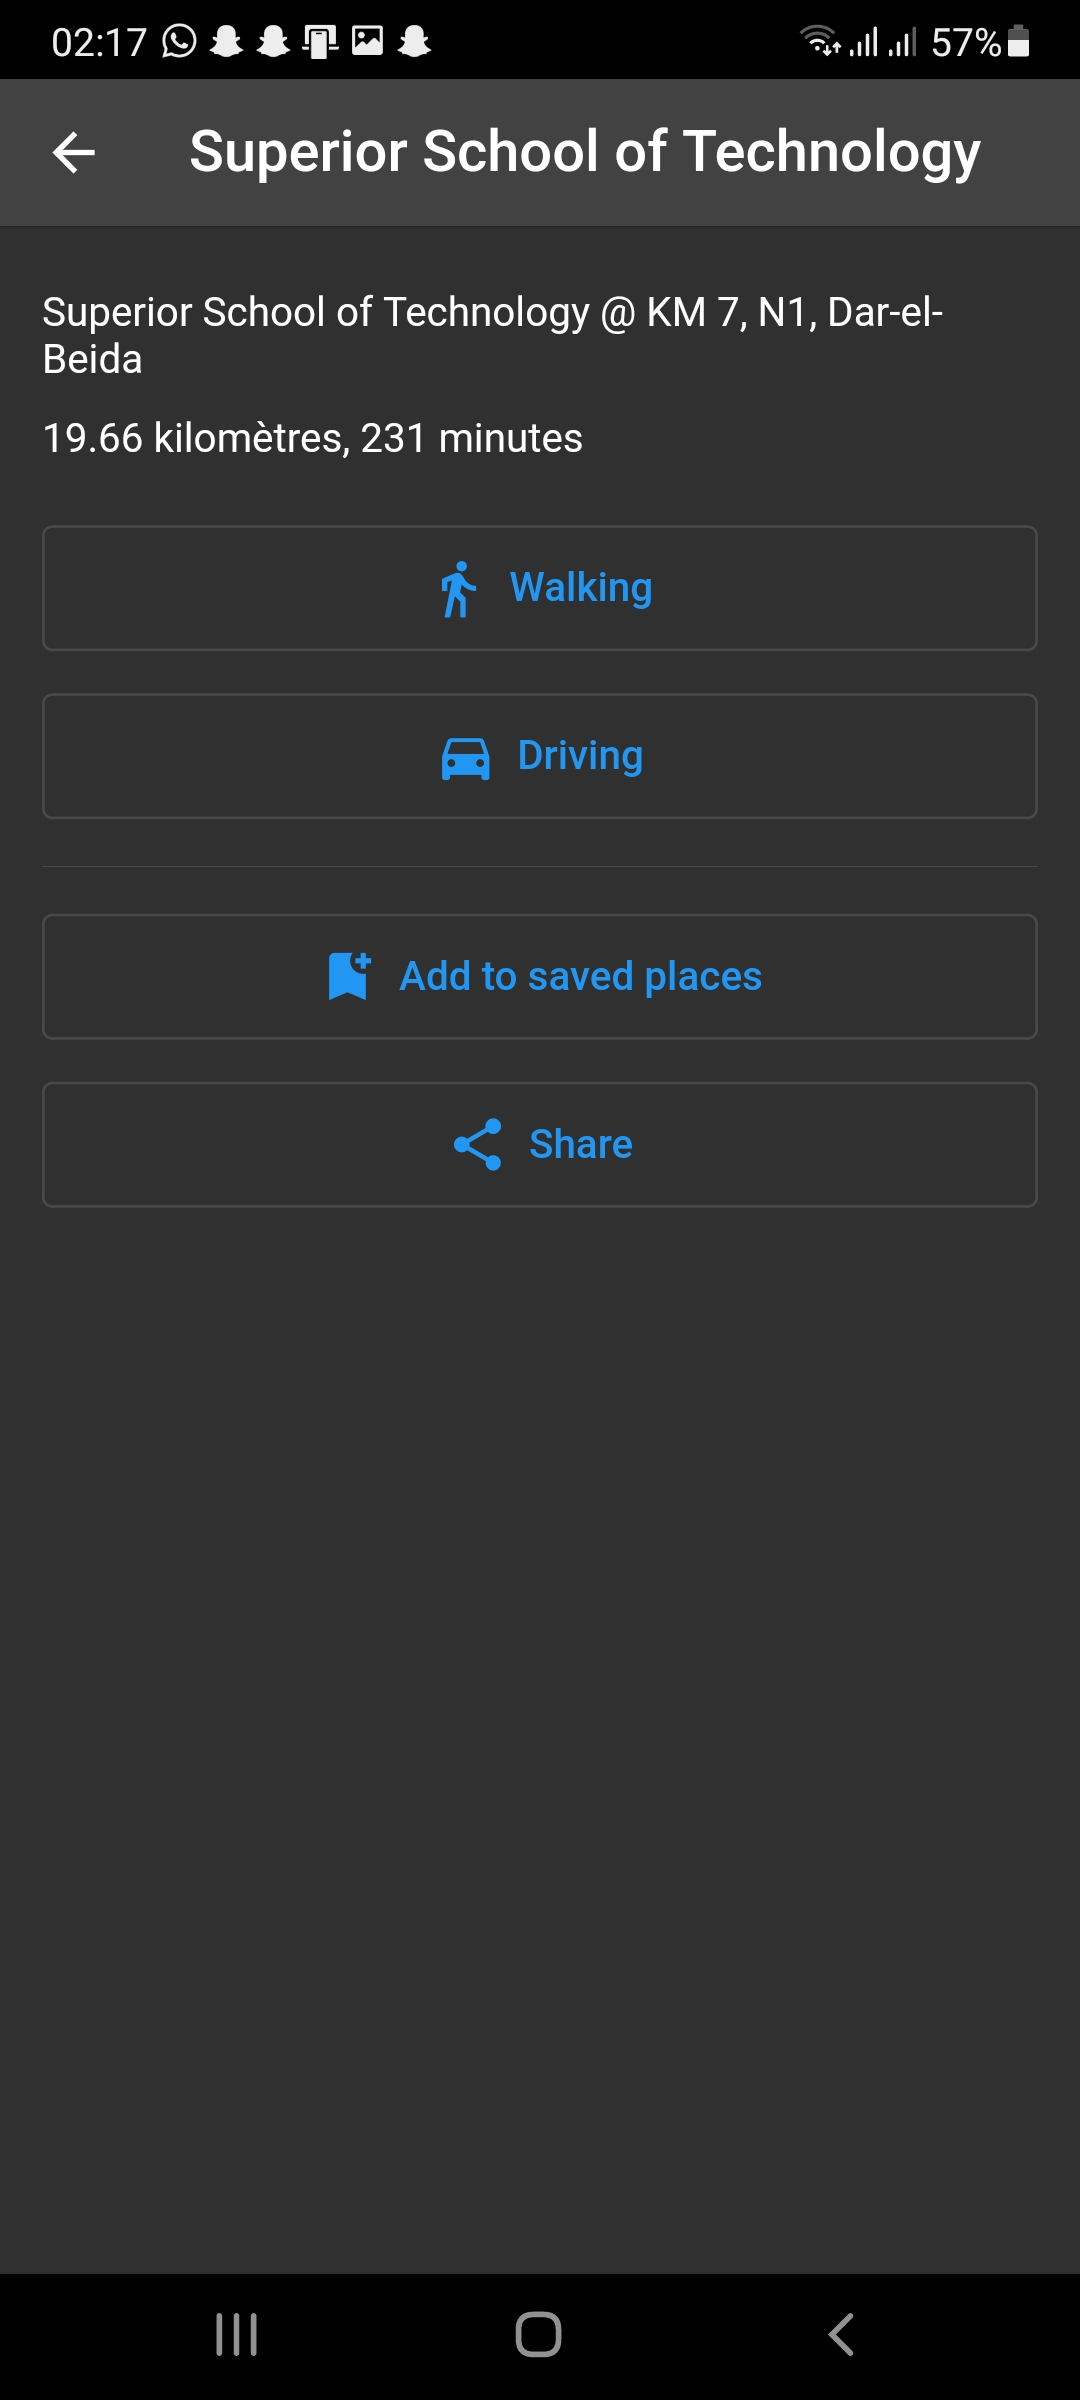
\includegraphics[width=\textwidth]{assets/app/search/infos.jpg}
         \caption{Endroit sélectionné}
    \end{subfigure}
    \caption{Recherche d'un endroit voulu}
\end{figure}

\FloatBarrier

\subsubsection{Les endroits favoris}

L'utilisateur peut ajouter un endroit à sa liste des endroits favoris afin de faciliter le retrouver 
\begin{figure}[!htbp]
    \centering
    \begin{subfigure}[t]{.3\linewidth}
        \centering
         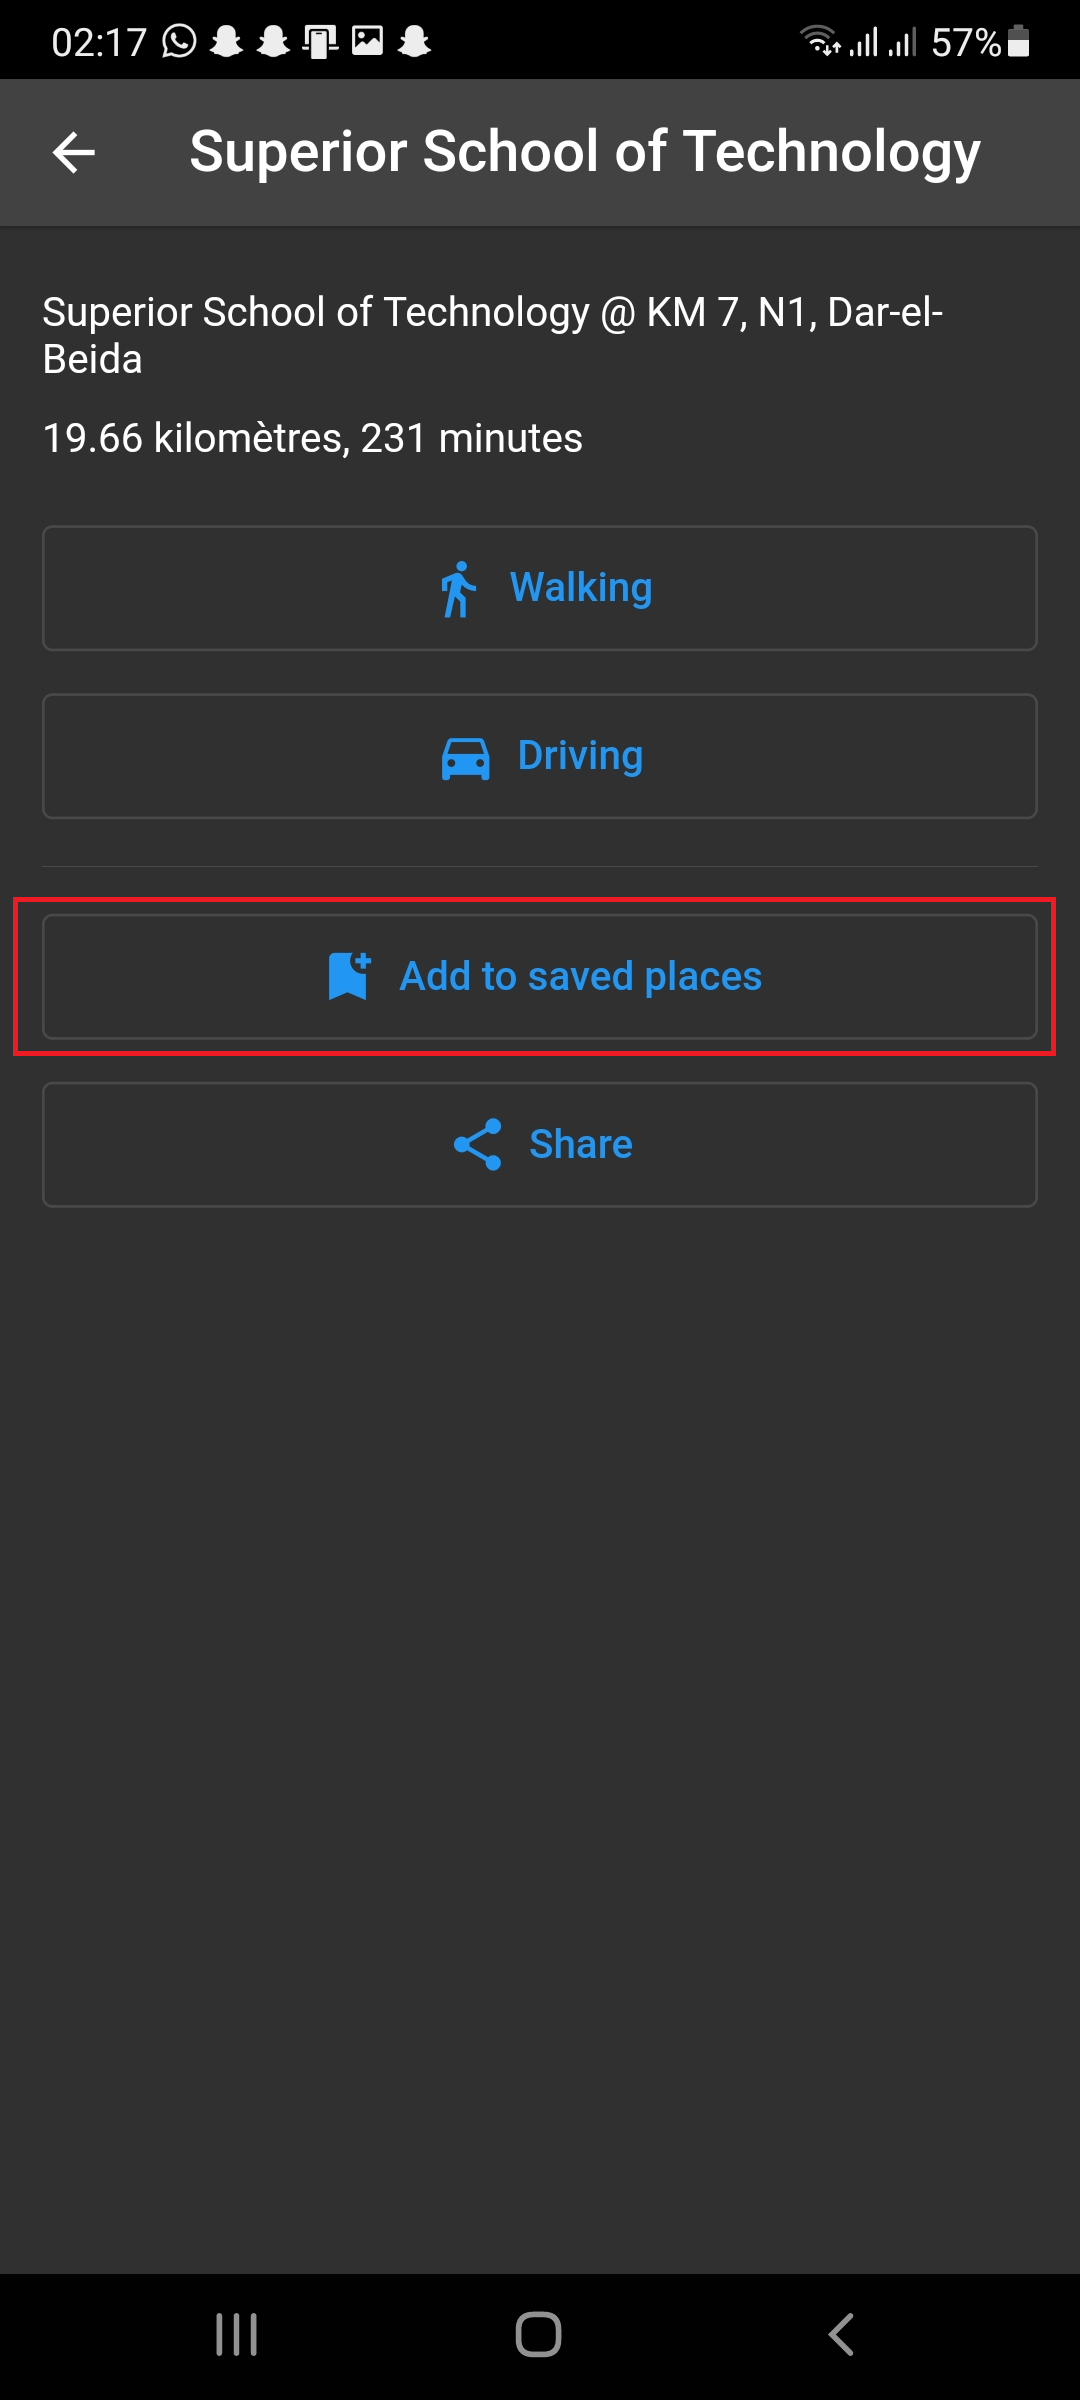
\includegraphics[width=\textwidth]{assets/app/favourites/before.png}
        \caption{}
    \end{subfigure}
    \hfill
    \begin{subfigure}[t]{.3\linewidth}
        \centering
         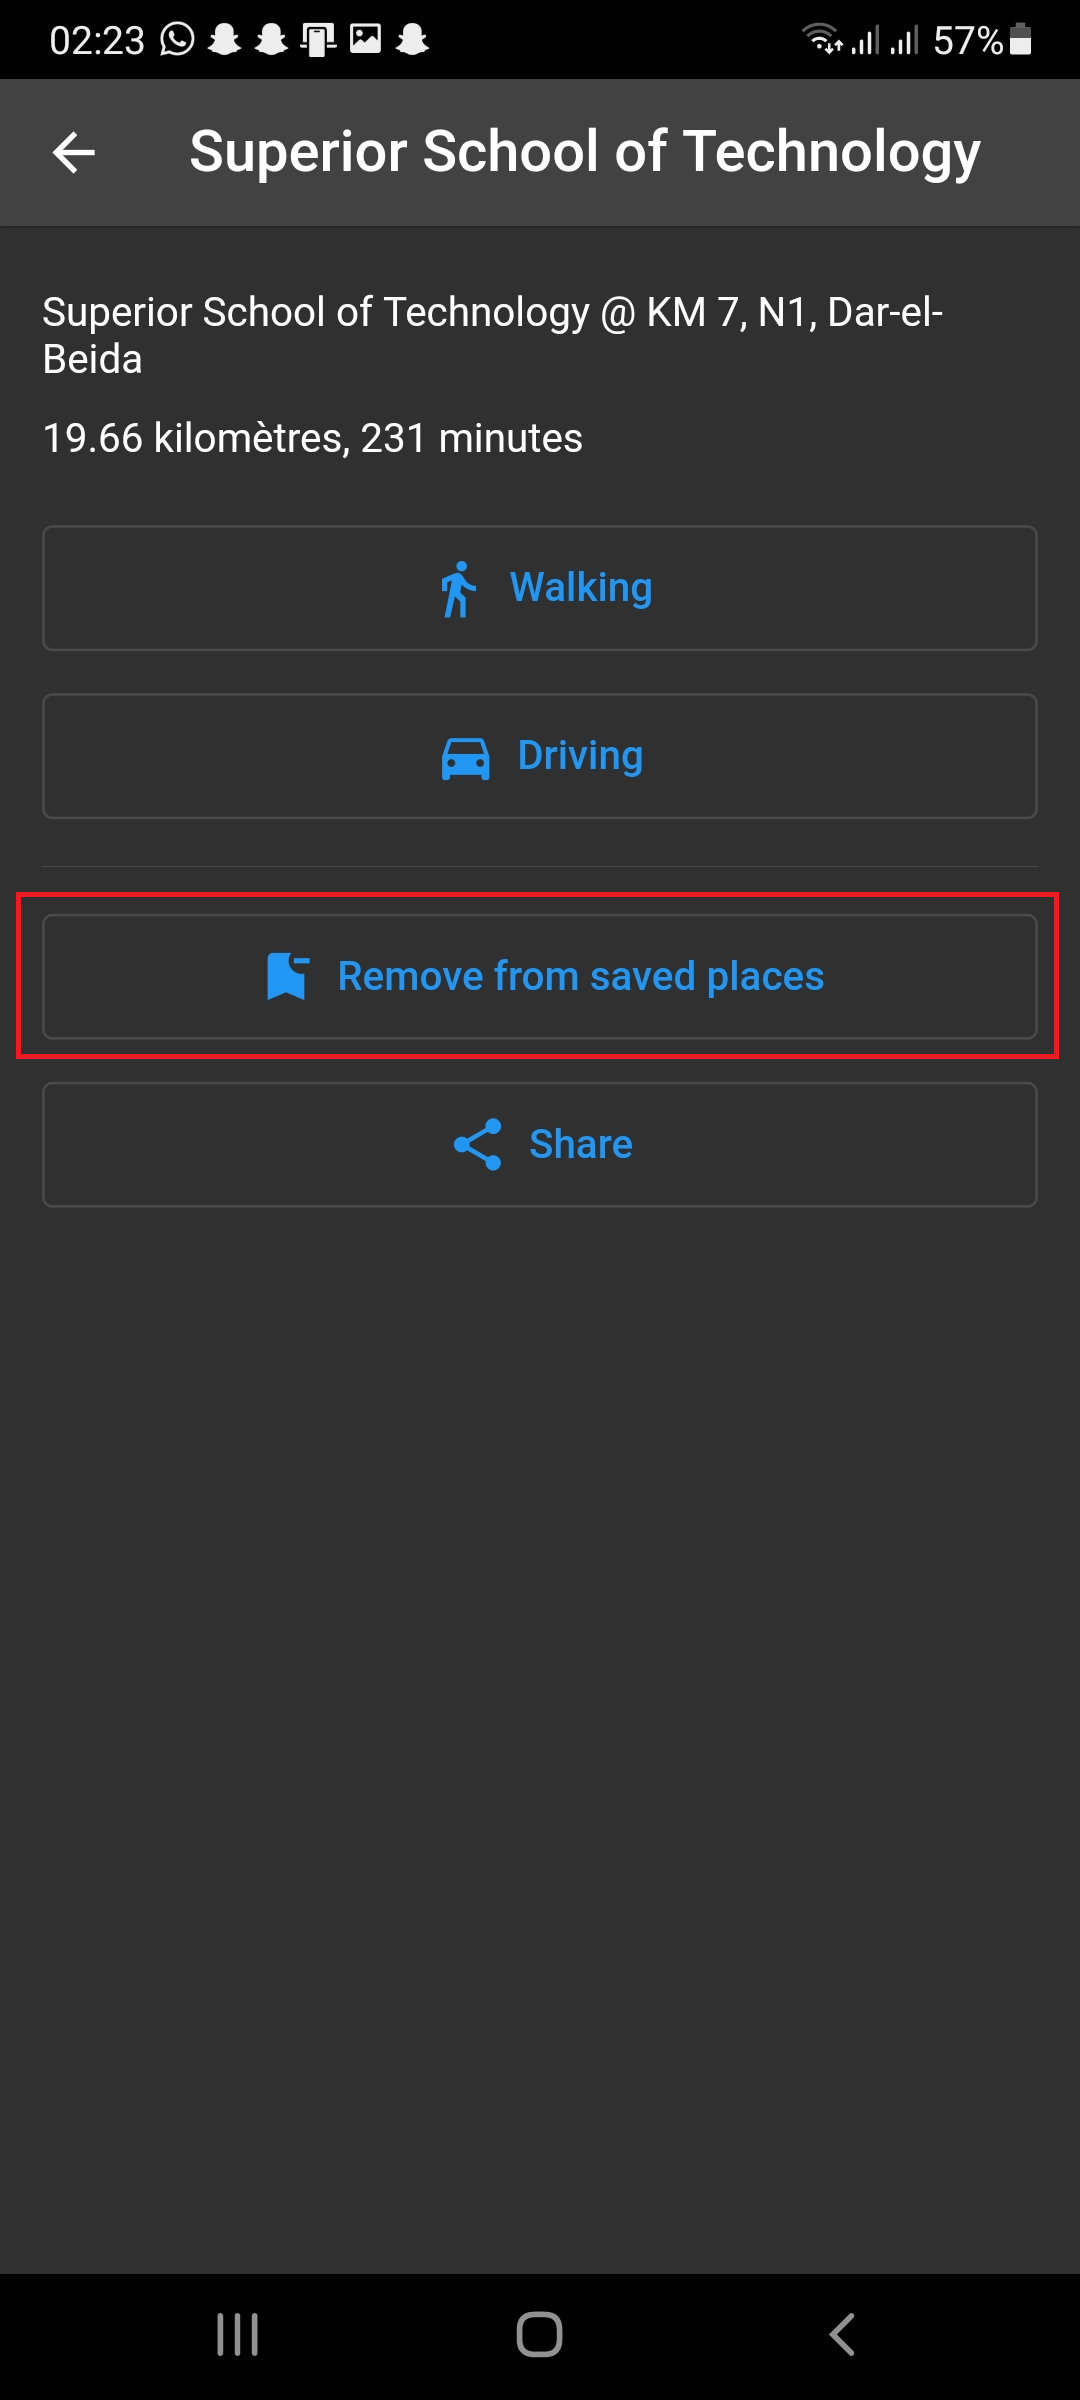
\includegraphics[width=\textwidth]{assets/app/favourites/after.png}
         \caption{Endroit ajouté a la liste des endroits favoris}
    \end{subfigure}
    \hfill
    \begin{subfigure}[t]{.3\linewidth}
        \centering
         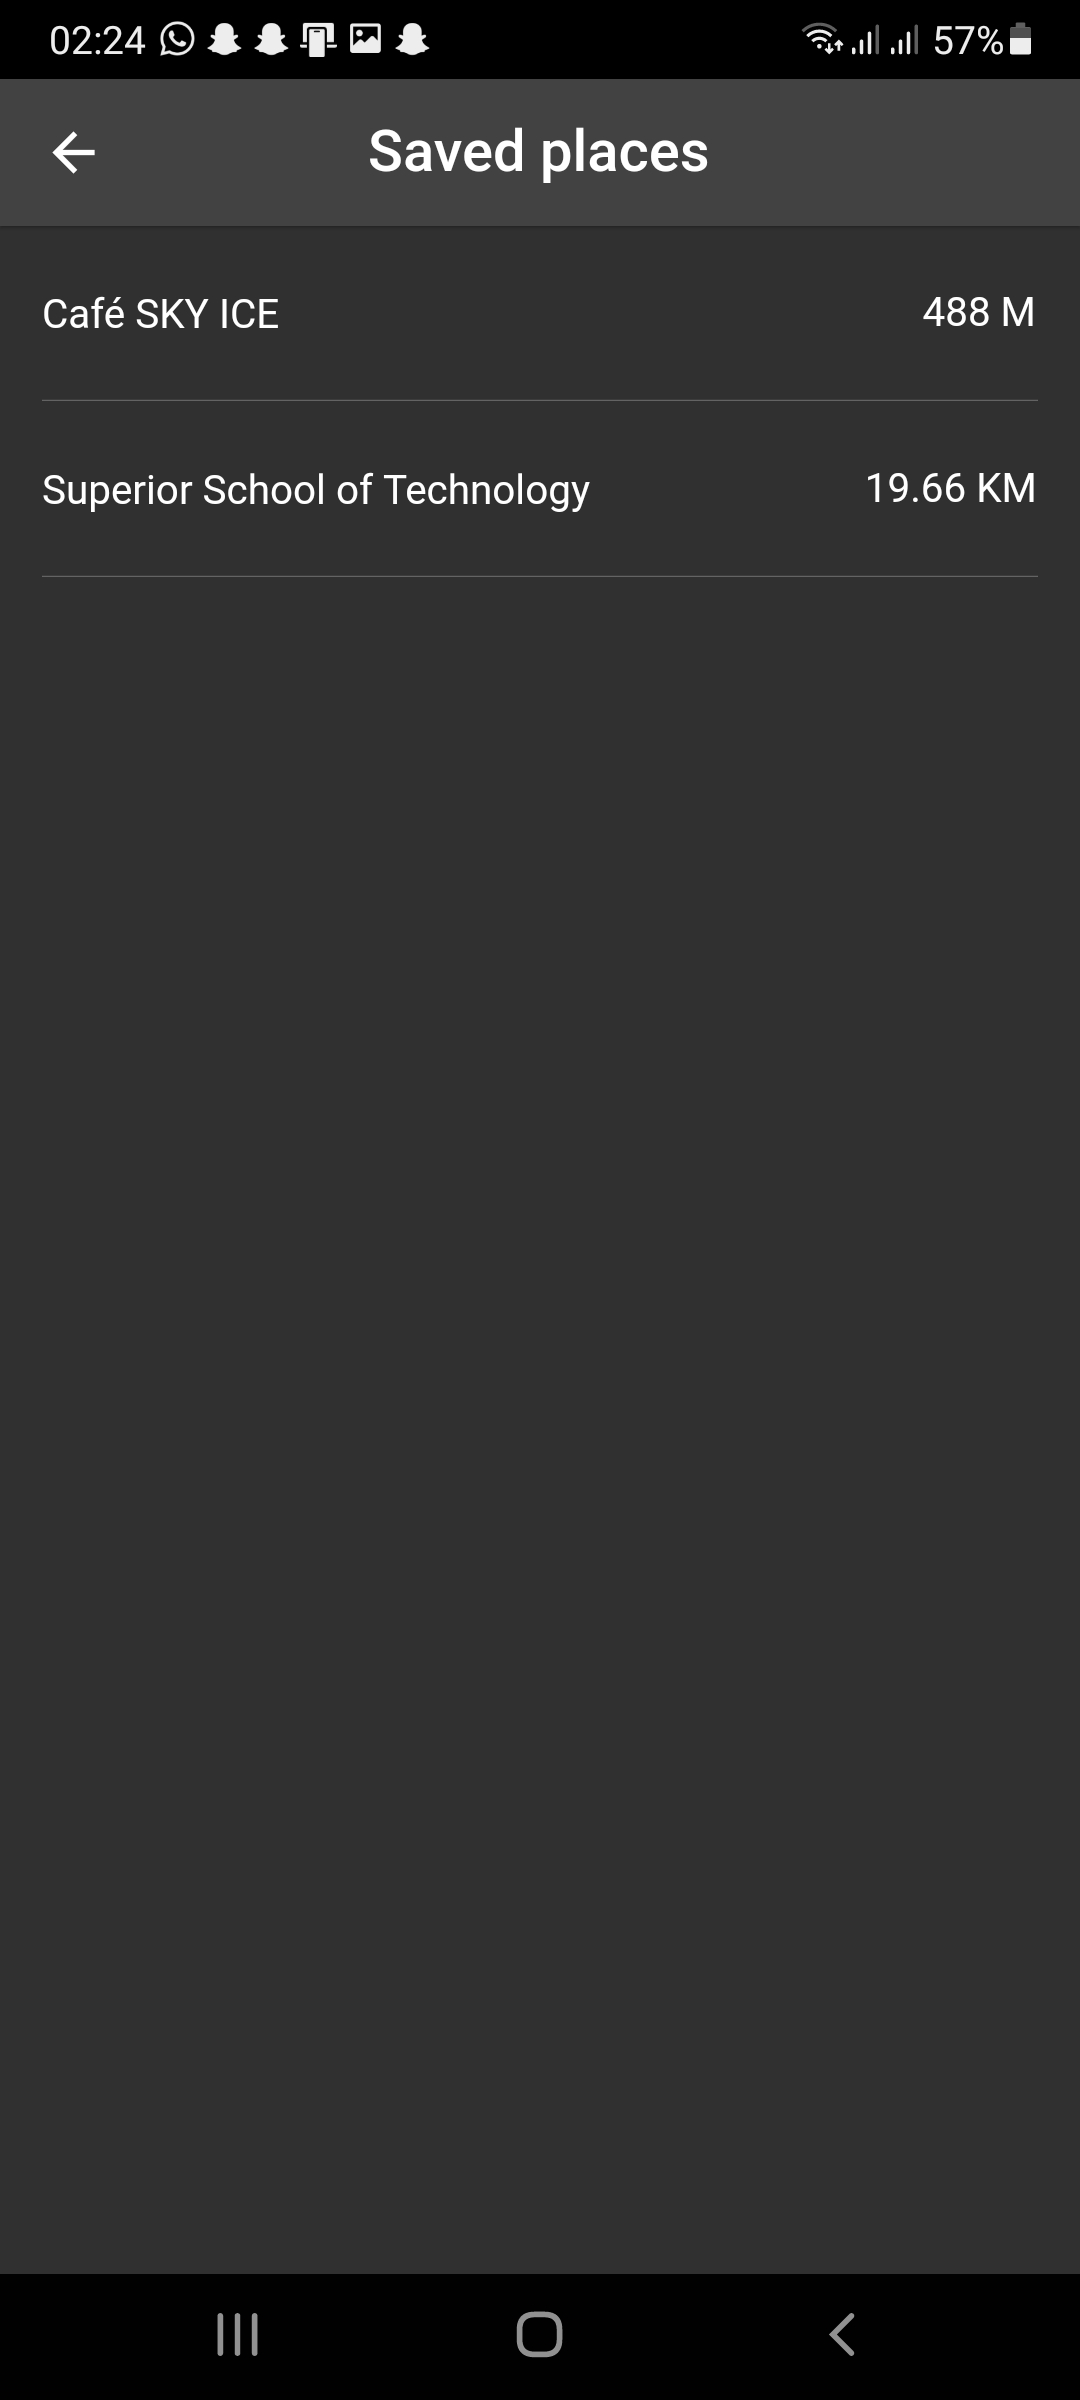
\includegraphics[width=\textwidth]{assets/app/favourites/result.jpg}
         \caption{Liste des endroits favoris}
    \end{subfigure}
    \caption{Les endroits favoris}
\end{figure}

\FloatBarrier

\subsubsection{Partage des endroits}

\begin{figure}[!htbp]
    \centering
    \begin{subfigure}[t]{.45\linewidth}
        \centering
         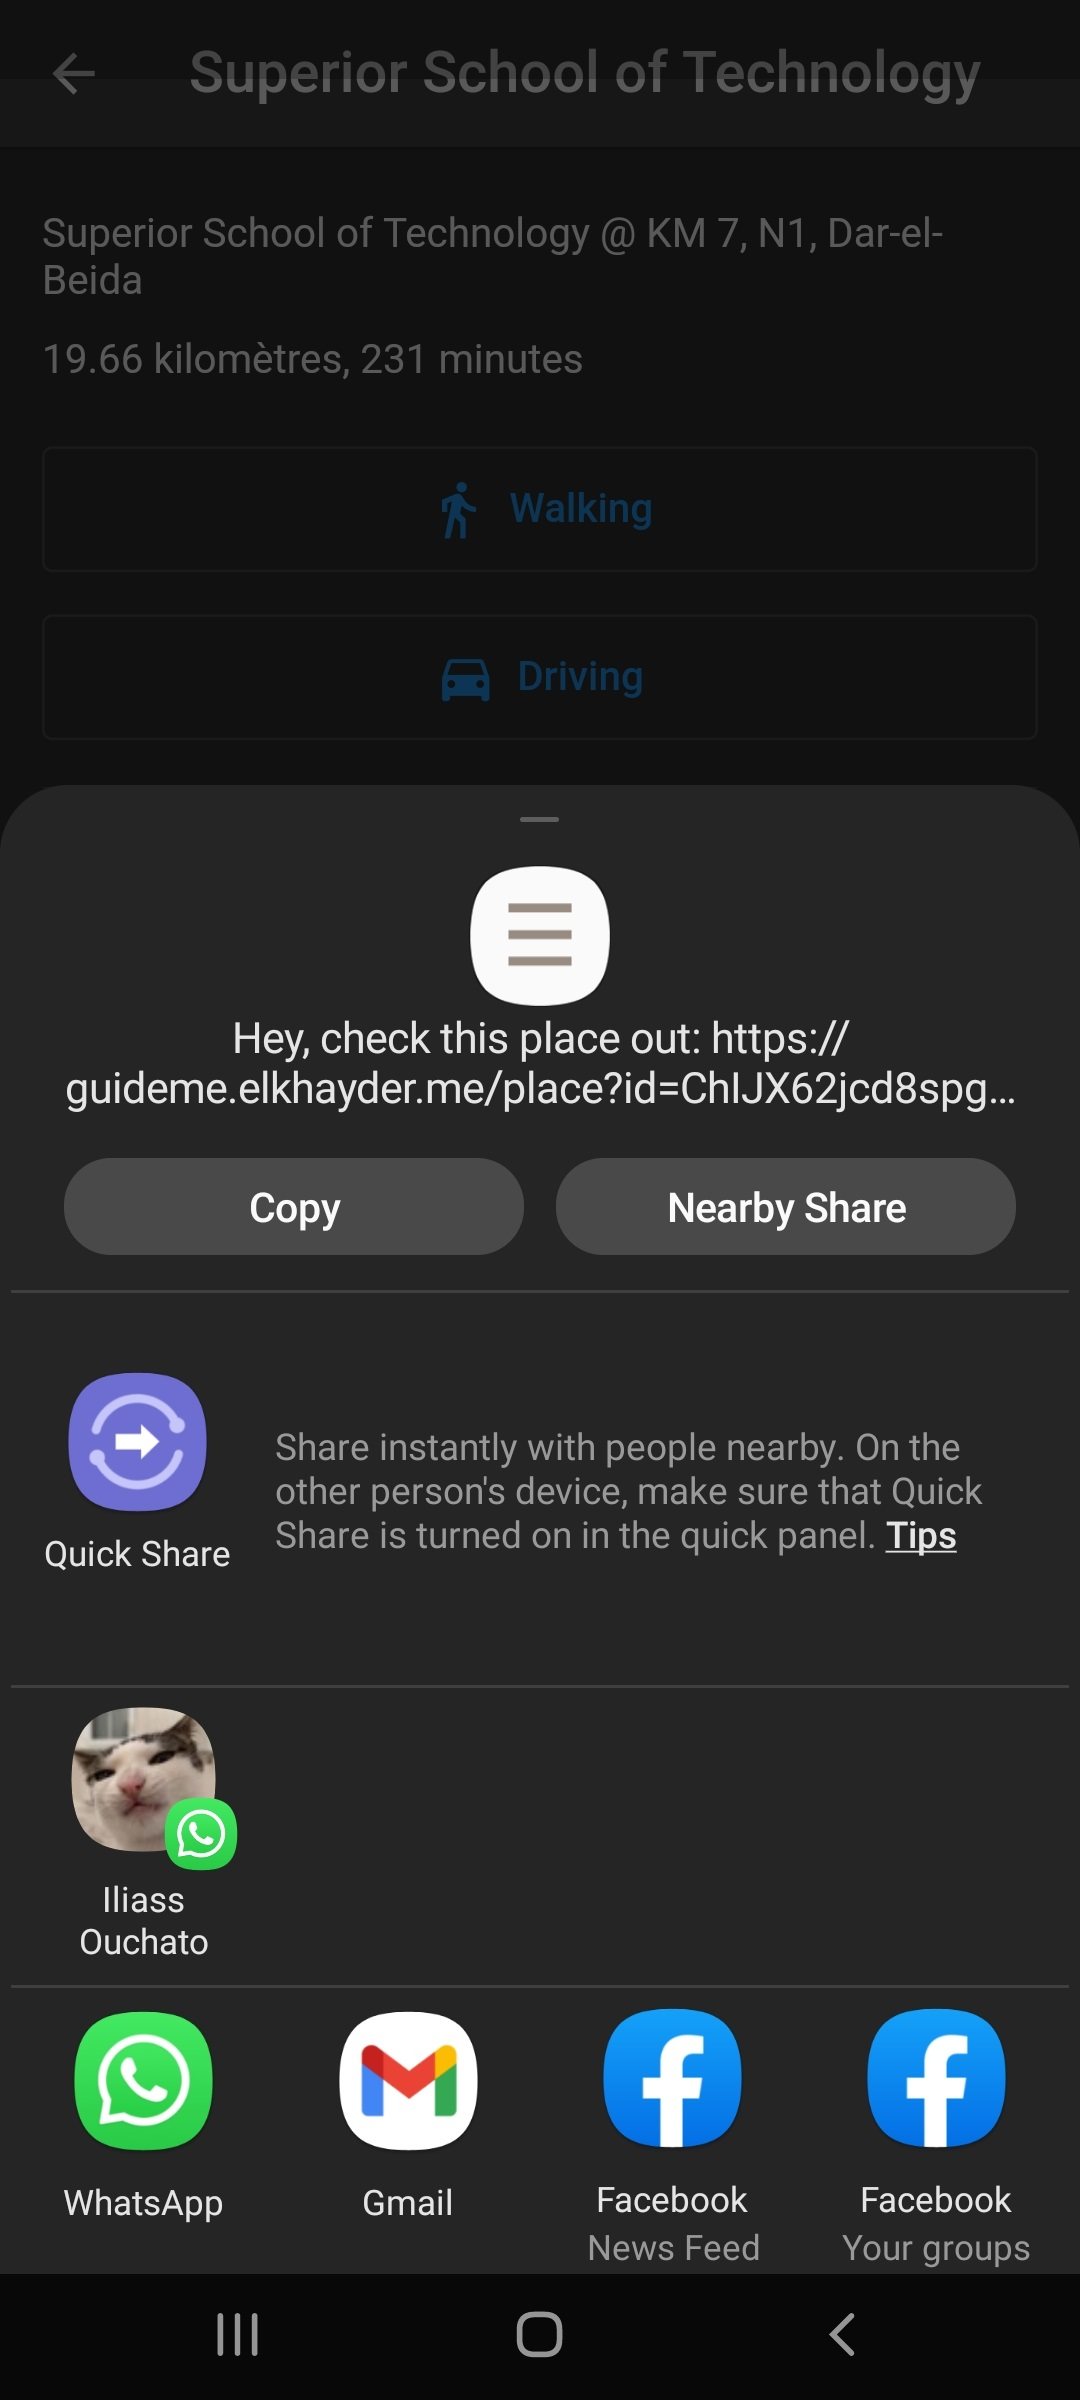
\includegraphics[width=\textwidth]{assets/app/share/share.jpg}
        \caption{Les options disponibles pour partager le lien d'endroit}
    \end{subfigure}
    \hfill
    \begin{subfigure}[t]{.45\linewidth}
        \centering
         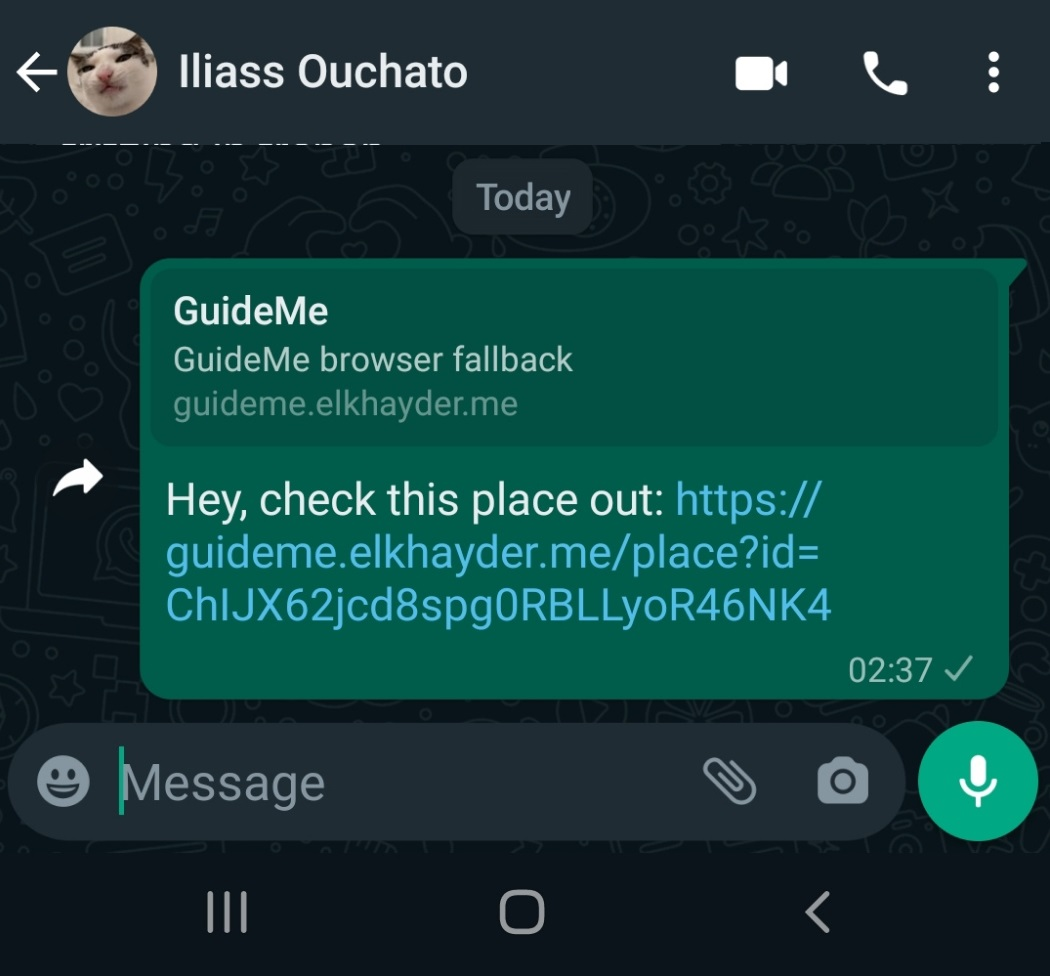
\includegraphics[width=\textwidth]{assets/app/share/shared.jpg}
         \caption{Endroit partagé}
    \end{subfigure}
    \caption{Partage des endroits}
\end{figure}

\FloatBarrier

Le lien partagé ouvre l'application mobile sur la page correspondant à l'endroit, au cas si l'application n'est pas installée, ce lien va rediriger vers le site web créé dans le chapitre \ref{website}.

Le lient contient la valeur \verb|place_id| qu'on a parlé dans le chapitre \fullref{place-details}, cette valeur sera utilisé pour trouver les informations de cet endroit.

\subsubsection{La navigation}

\subsection{Localisation de la place en cas de perte}

L’application téléphonique sera responsable d’obtenir la position actuelle de l’utilisateur à l’aide des capteurs \acrshort{GPS} intégrés du téléphone. \\
Une fois que nous avons les coordonnées de l’utilisateur, nous récupérons les contacts d’urgence et le message d’urgence des paramètres. Puis Nous joignons un lien Google Maps à la latitude et la longitude de l’utilisateur avec le message d’urgence, et on l’envoie.

\begin{figure}[!htbp]
    \centering
    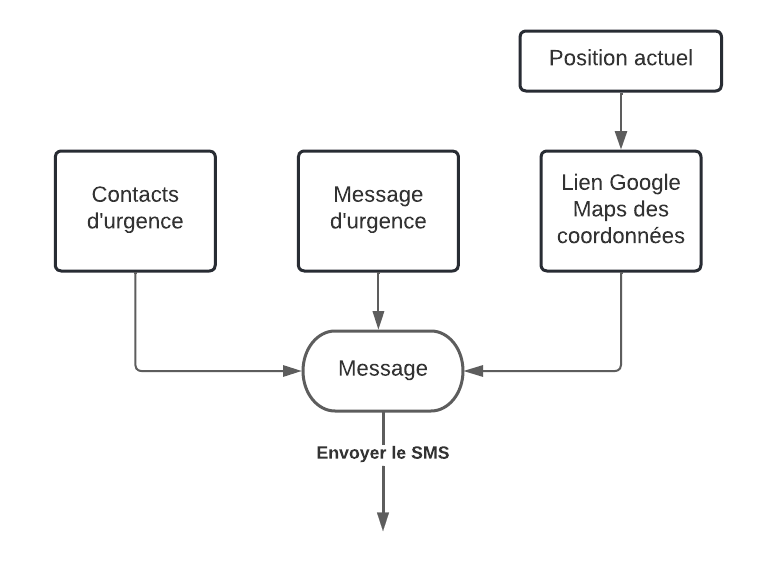
\includegraphics[width=.7\linewidth]{assets/SMS/diagramme simplified.png}
    \caption{Logigramme de l'SMS en cas de perte}
\end{figure}

\FloatBarrier

\begin{code}
\begin{minted}[frame=single,
               framesep=3mm,
               linenos=true,
               xleftmargin=21pt,
               tabsize=4, fontsize=\small, breaklines]{dart}
class SendCurrentLocationSMS implements BluetoothPayloadHandler {
  final Telephony telephony = Telephony.instance;
  final LocationService location = LocationService();

  @override
  String command = "SEND_LOCATION_SMS";

  @override
  void handle(List<String> args) async {
    var currentLocation = await location.updateCurrentLocation();
    var prefs = await SharedPreferences.getInstance();
    String message = prefs.getString("emergencyMessage") ?? Constants.defaultEmergencyMessage;
    List<EmergencyContact> contacts = await Helpers.fetchEmergencyContacts();

    if (currentLocation?.longitude != null && currentLocation?.latitude != null) {
      message += "https://www.google.com/maps/search/?api=1&query=${currentLocation
      !.latitude!.toString()}%2C${currentLocation.longitude!.toString()}";
    }

    if (contacts.isEmpty) {
      await Helpers.speak(
        "You don't have any emergency contacts, please add at least one in the settings menu.",
      );
      return;
    }

    for (var c in contacts) {
      await telephony.sendSms(
        to: c.phone,
        message: message,
      );
    }

    await Helpers.speak(
      "Location SMS sent to ${contacts.length} ${contacts.length == 1 ? "person" : "people"}",
    );
  }
}
\end{minted}
\caption{Expéditeur d'SMS d'urgence}
\end{code}

\begin{figure}[!htbp]
    \centering
    \begin{subfigure}[t]{.45\linewidth}
        \centering
         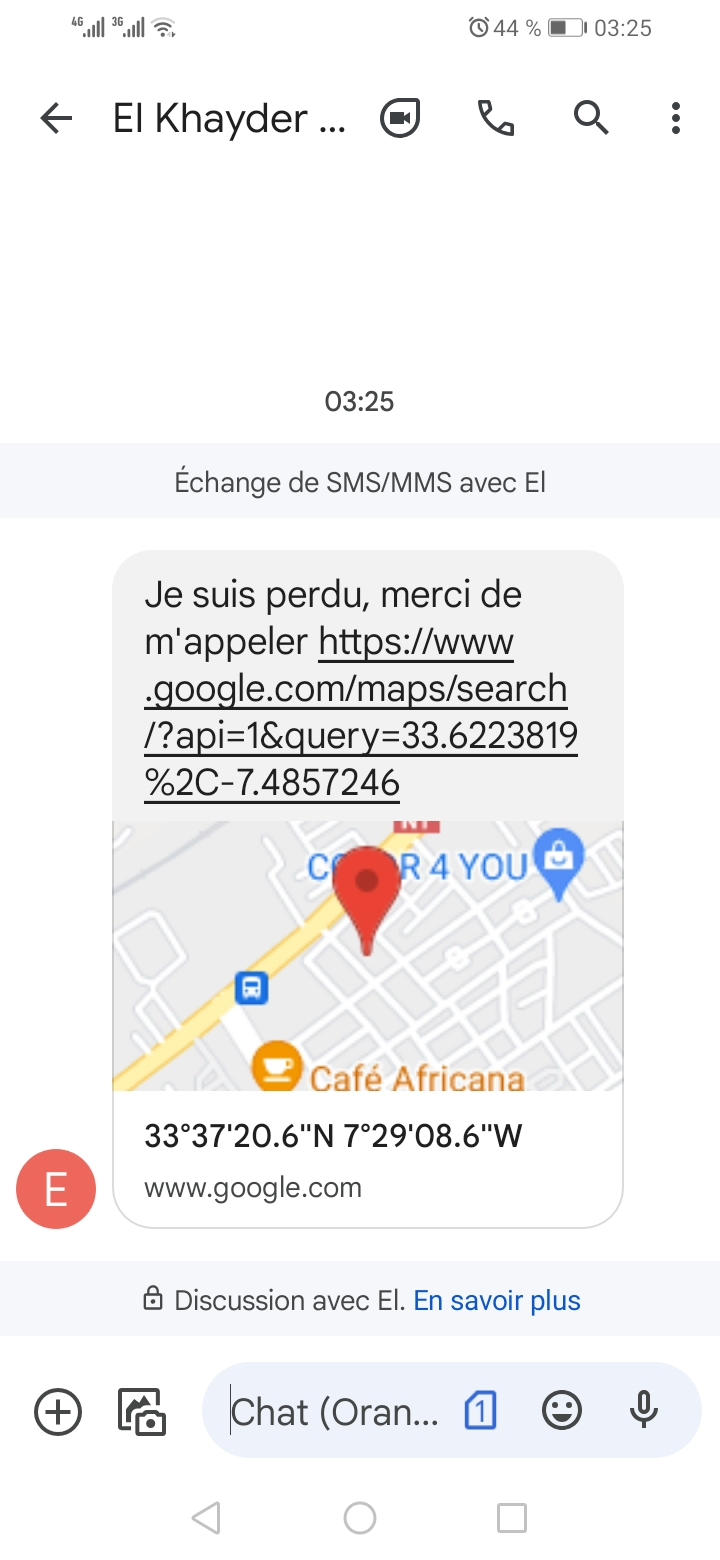
\includegraphics[width=\textwidth]{assets/SMS/sms.jpg}
        \caption{SMS envoyé}
    \end{subfigure}
    \hfill
    \begin{subfigure}[t]{.45\linewidth}
        \centering
         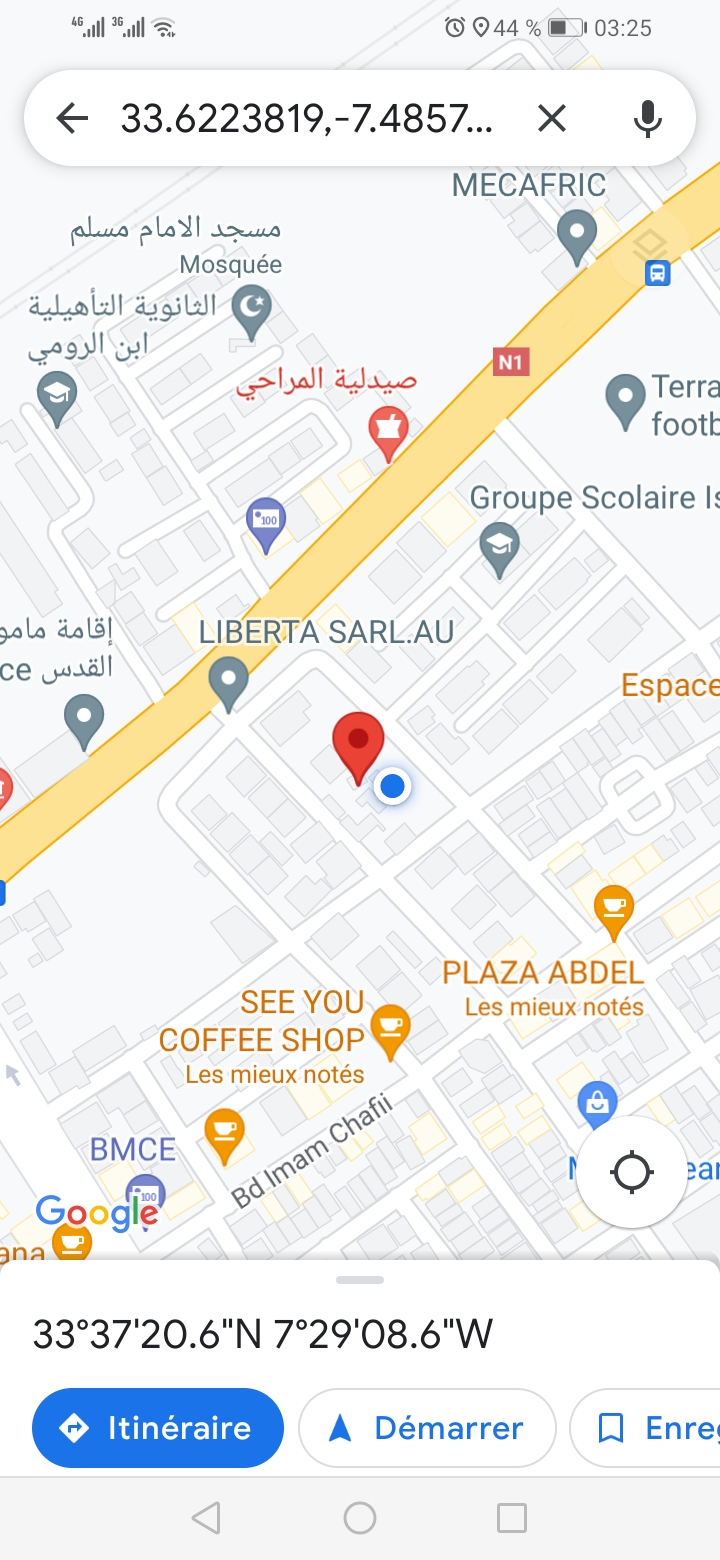
\includegraphics[width=\textwidth]{assets/SMS/location.jpg}
         \caption{Position partagée}
    \end{subfigure}
    \caption{SMS de position actuelle en cas de perte}
\end{figure}

\FloatBarrier

On peut déclencher cette action à partir du téléphone directement, ou par les boutons de commande sur la canne à travers la communication Bluetooth entre les deux.

\subsection{Trouver le téléphone avec la canne et vice-versa}

En utilisant la canne, on peut lancer la sonnerie du téléphone pour que l'utilisateur peut le trouver facilement, comme on peut aussi lancer la sonnerie de la canne d'après le téléphone à condition que les deux sont connecte entre eux avec Bluetooth

\section{Le site web}
\label{website}

Le site va fournir au destinataire les informations de l'endroit partagée au cas si l'application mobile GuideMe n'est pas installée sur son téléphone.

\begin{code}
\begin{minted}[frame=single, framesep=3mm, linenos=true, xleftmargin=21pt, tabsize=4, fontsize=\small, breaklines]{typescript}
import React, { useEffect, useState } from "react";

type Place = {
   id: string;
   name: string;
   address: string;
   location: {
      lat: string;
      lng: string;
   };
};

const App = () => {
   const [place, setPlace] = useState<Place | null>(null);
   const [error, setError] = useState<String | null>(null);
   const [isLoading, setIsLoading] = useState(true);

   useEffect(() => {
      fetchPlaceInfos();
   }, []);

   const fetchPlaceInfos = async () => {
      const currentUrl = new URL(window.location.href);

      const apiEndpoint = new URL(
         "https://private-no-cors-proxy.herokuapp.com/https://maps.goog
         leapis.com/maps/api/place/details/json"
      );

      apiEndpoint.searchParams.append(
         "place_id",
         currentUrl.searchParams.get("id") ?? ""
      );

      apiEndpoint.searchParams.append(
         "key",
         "PRIVATE_KEY"
      );

      const request = await fetch(apiEndpoint.toString())
         .then((x) => x.json())
         .catch((e) => {
            setError(
               "We encountered an error while loading place infos, try to refresh the page."
            );
            return null;
         })
         .finally(() => setIsLoading(false));

      if (!request) return;

      if (request.status === "INVALID_REQUEST") {
         setError(
            "Seems like the link is broken, make sure you copied the exact one you received."
         );
         return;
      }

      setPlace({
         id: request.result.place_id,
         name: request.result.name,
         address: request.result.formatted_address,
         location: request.result.geometry.location,
      });

      document.title = `${request.result.name} — GuideMe`;
   };

   return (
      <section id="head">
         {isLoading && (
            <div className="lds-ring">
               <div />
               <div />
               <div />
               <div />
            </div>
         )}
         {error && <h3 className="error">{error}</h3>}
         {place && (
            <>
               <h1 className="title">{place?.name}</h1>
               <h2 className="address">{place?.address}</h2>
               <div className="row">
                  <a href={`https://guideme.elkhayder.me/?id=${place?.id}`}>
                     <button className="purple">
                        <i className="fa-solid fa-location-crosshairs fa-2x" />
                        <span>Open in GuideMe</span>
                     </button>
                  </a>
                  <a
                     href="https://github.com/elkhayder/SmartCane-PFE-2022"
                     target="_blank"
                     rel="noreferrer"
                  >
                     <button className="blue">
                        <i className="fa-brands fa-android fa-2x" />
                        <span>Download app for Android</span>
                     </button>
                  </a>
                  <a
                     href={`https://maps.google.com?q=
                     ${place.location.lat},${place.location.lng}`}
                     target="_blank"
                     rel="noreferrer"
                  >
                     <button className="green">
                        <i className="fa-solid fa-map fa-2x" />
                        <span>Open in Maps</span>
                     </button>
                  </a>
               </div>
            </>
         )}
      </section>
   );
};

export default App;

\end{minted}
\caption{Website}
\end{code}

\begin{figure}[!htbp]
    \centering
    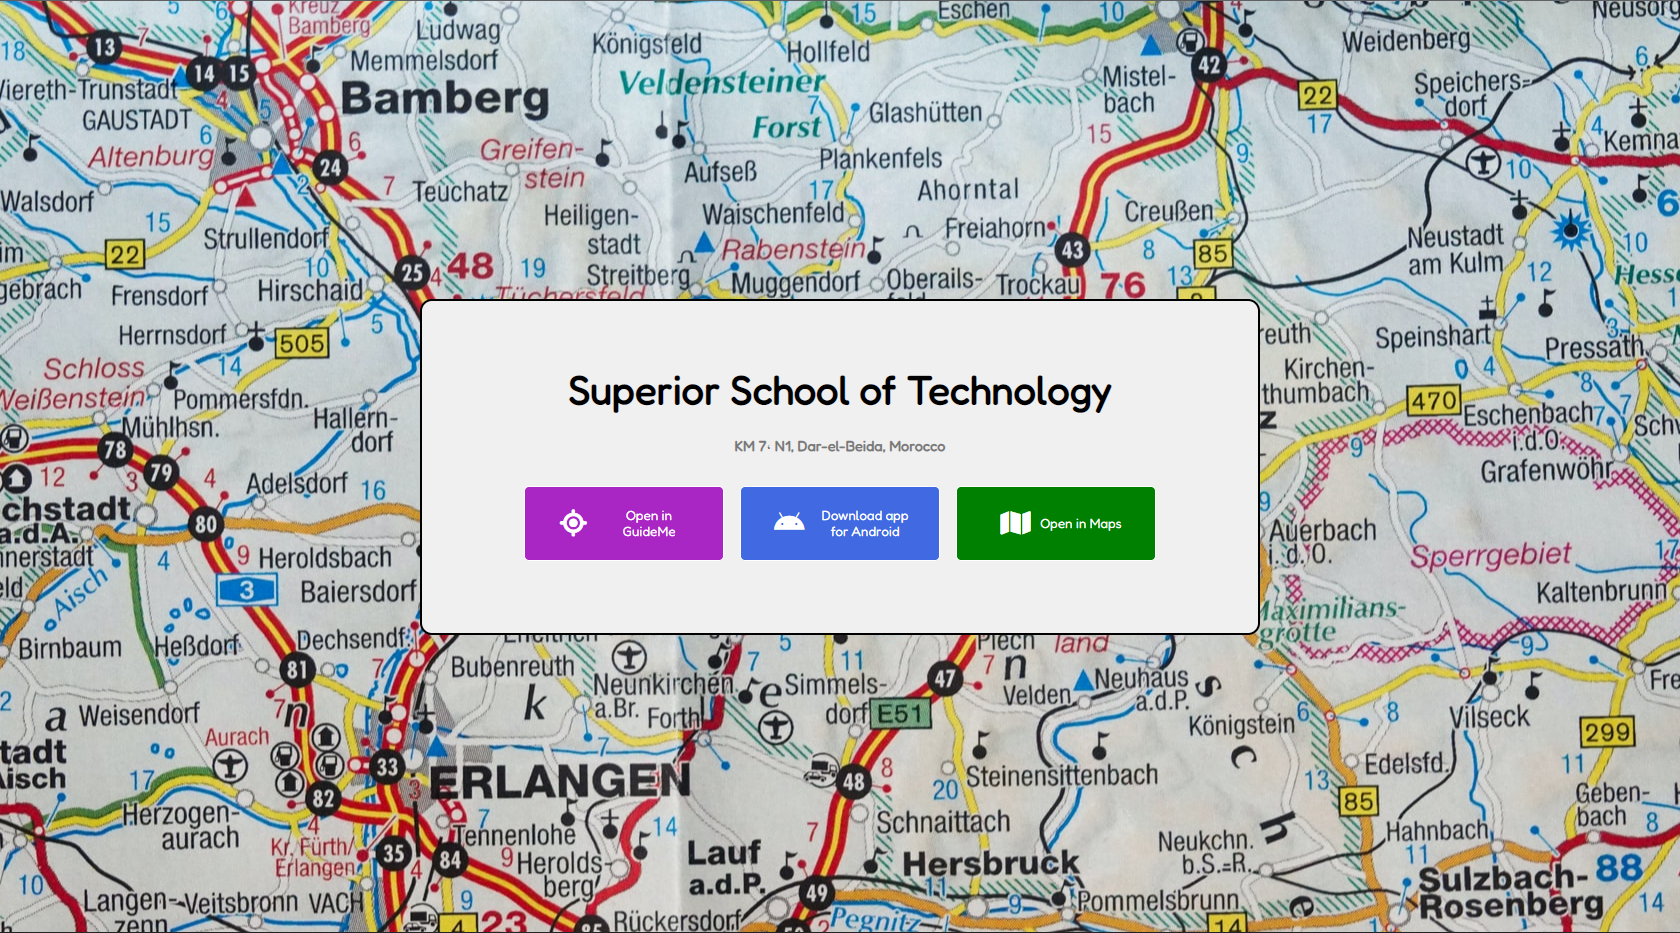
\includegraphics[width=\textwidth]{assets/website/web.png}
    \caption{Website: Version Web}
\end{figure}

\begin{figure}[!htbp]
    \centering
    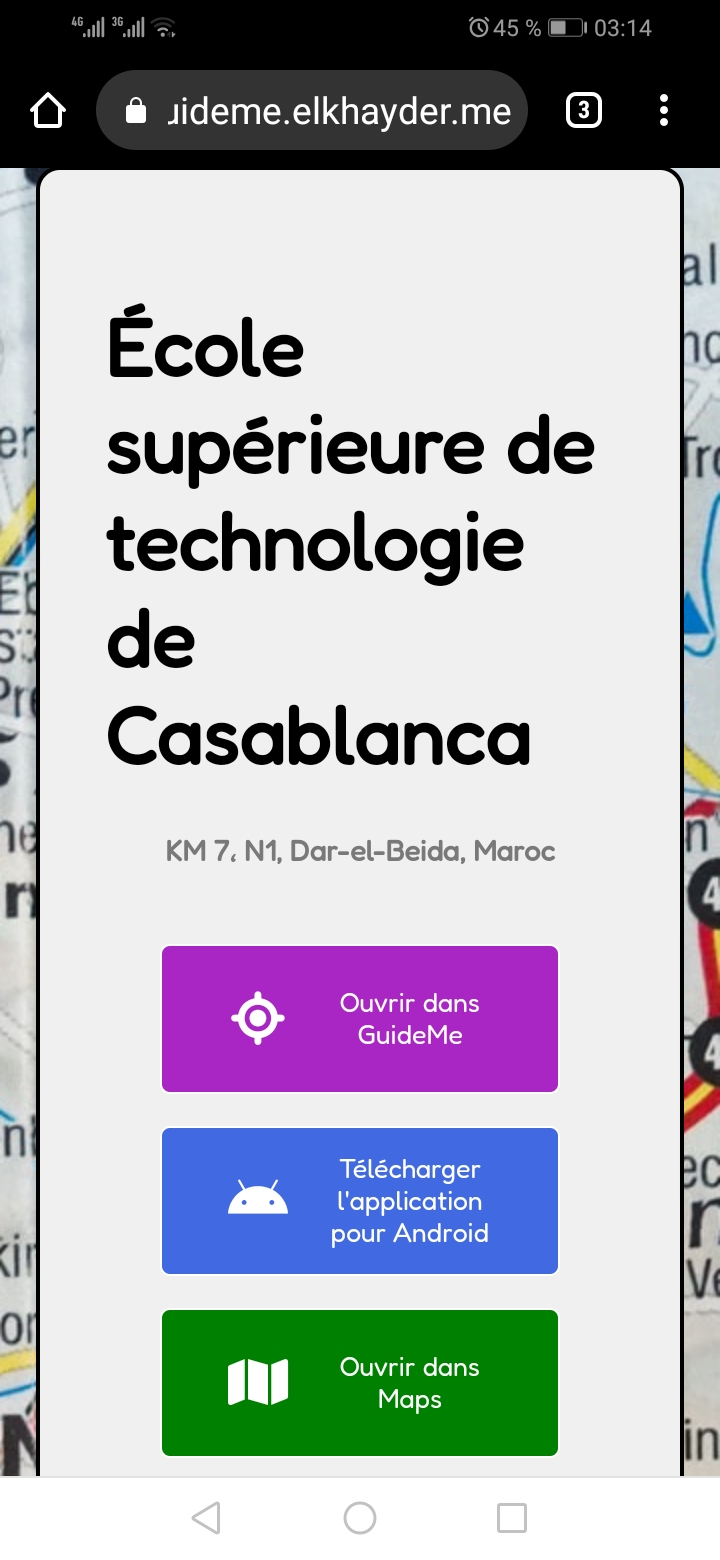
\includegraphics[height=.8\textheight]{assets/website/mobile.jpg}
    \caption{Website: Version mobile}
\end{figure}

\FloatBarrier

\section{Conception de la canne}

\subsection{Introduction}
Pour s’assurer que notre canne peut être facilement utilisé comme appareil portatif qui va accompagner l’utilisateur pendant ses promenades, qui va rendre sa vie plus facile plutôt que difficile en étant un fardeau, nous avons dû faire un design ergonomique et léger. 

Pour satisfaire cela, les composants utilisés dans la fabrication de la canne ont dû travailler ensemble dans un boîtier compact c’est pourquoi nous avons conçu des circuits imprimés pour faire exactement cela et nous avons fait un boîtier qui va tenir ces \acrshort{PCB}s d’une manière efficace pour économiser le maximum d’espace possible afin que nous puissions assurer un appareil portable qui sera fonctionnel et attrayant pour l’utilisateur en même temps.

\subsection{Conception des circuits imprimés}

\subsubsection{Les circuits imprimés}
Une carte de circuit imprimé (PCB) est une structure sandwich stratifiée de couches conductrices et isolantes. Les PCB ont deux fonctions complémentaires. La première consiste à apposer des composants électroniques aux endroits désignés sur les couches extérieures au moyen de la soudure. Le second est de fournir des connexions électriques fiables (et aussi des circuits ouverts fiables) entre les bornes du composant d’une manière contrôlée souvent appelée conception de circuits imprimés.

\begin{figure}[!htbp]
    \centering
    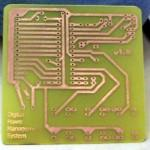
\includegraphics[width=4cm]{assets/conception1/img16.jpg}
    \caption{Un exemple d'un PCB}
\end{figure}

\FloatBarrier

\subsubsection{Design}
Pour porter nos composants électroniques à la vie dans la forme physique on fait la conception à l’aide d’un logiciel spécifique dédié pour la réalisation.

\verb|Altium Designer| a été le premier logiciel de conception de circuits imprimés choisi, c’est un éditeur complet pour les schémas électroniques utilisés par les professionnels et les ingénieurs de conception de circuits imprimés dans toutes sortes d’industries telles que les télécommunications.

\vspace{1cm}

\begin{figure}[!htbp]
    \centering
    
\includegraphics[width=6cm]{assets/conception1/img19.jpg}
\end{figure}


\begin{figure}[!htbp]
    \centering
    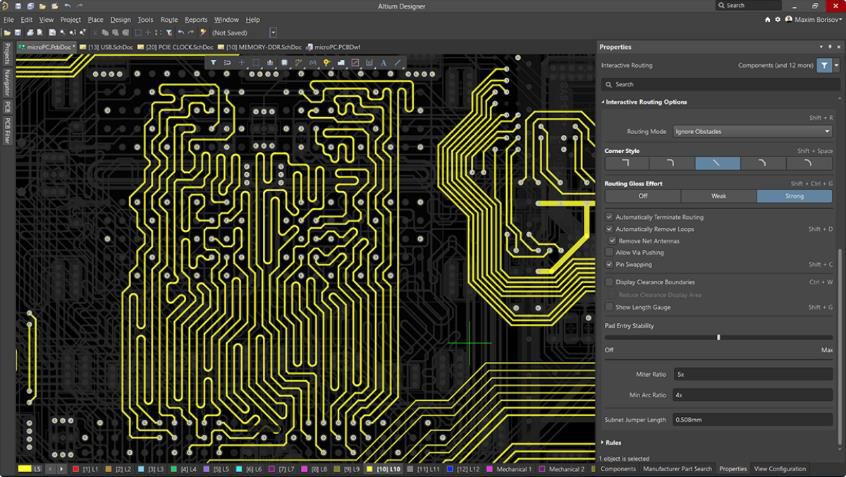
\includegraphics[width=.8\textwidth]{assets/conception1/img21.jpg}
    \caption{Interface du logiciel Altium Designer}
\end{figure}

\FloatBarrier

Mais pendant que nous travaillions sur le logiciel nous avons rencontré tellement des difficultés en termes de facilité d’utilisation car c’était un environnement assez intense pour nous en tant que des étudiants qui n’ont pas beaucoup d’expérience dans la conception des PCBs, nous ne pouvions pas non plus nous permettre d’acheter une licence pour le logiciel alors nous avons utilisé une version craquée mais ce n’était pas stable il a continué à se planter et montrant des erreurs.

\vspace{1cm}

\begin{figure}[!htbp]
    \centering
    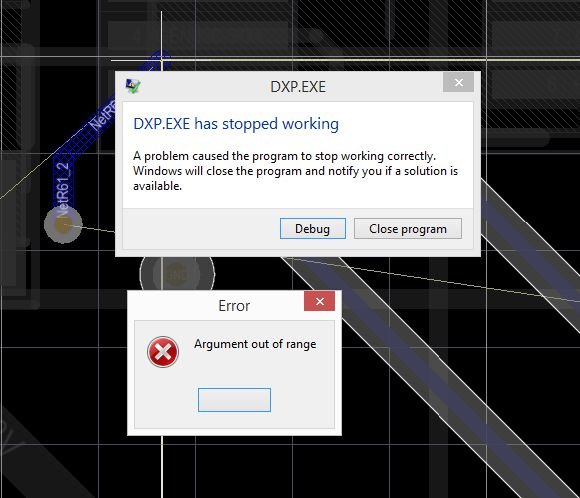
\includegraphics[width=.5\textwidth]{assets/conception1/img23.jpg}
    \caption{Problème de plantage de Altium Designer}
\end{figure}

\FloatBarrier

À d’autres moments, nous ne pouvions pas prendre le risque de perdre nos progrès, alors nous sommes passés à un autre logiciel que nous connaissons bien : Proteus : c’est un logiciel de conception de circuit imprimé et un simulateur de circuit qui est plus convivial pour les étudiants que Altium Designer qui est plus orienté pour les ingénieurs.  \\
On veut réaliser deux circuits électroniques : un circuit pour les boutons et un autre pour les autres composants (Le circuit Arduino)

\begin{figure}[!htbp]
    \centering
    
\includegraphics[width=.4\textwidth]{assets/conception1/img24.jpg}
\end{figure}

\begin{figure}[!htbp]
    \centering
    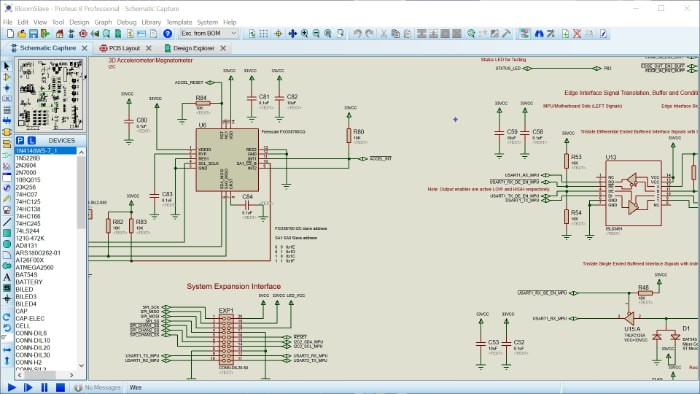
\includegraphics[width=.7\textwidth]{assets/conception1/schematicLrg.jpg}
    \caption{Interface Proteus}
\end{figure}

\FloatBarrier

\subsubsection{Circuit arduino}
Commençons par le circuit arduino : il y a eu beaucoup de changements qui se produisent tout au long de la réalisation ce circuit imprimé, donc nous allons commencer par le tout premier schéma:

\begin{figure}[!htbp]
    \centering
    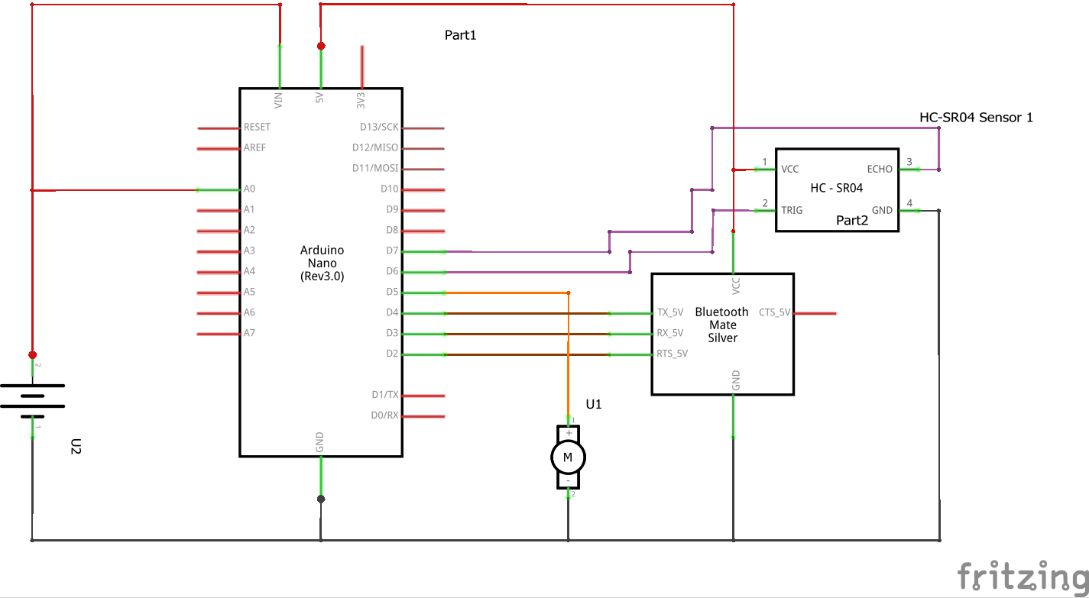
\includegraphics[width=.9\textwidth]{assets/conception1/img26.jpg}
    \caption{Circuit d'Arduino}
\end{figure}

\FloatBarrier

ce circuit a utilisé les principaux composants sur lesquels le projet était basé au début, nous avons travaillé sur le logiciel Fritzing pour avoir une idée générale de comment le circuit ressemblerait. Après nous avons réalisé le schéma ci-dessus sur Proteus en mode schematic capture.
\\[1cm]

\begin{figure}[!htbp]
    \centering
    
\includegraphics[width=.4\textwidth]{assets/conception1/img34.jpg}
\end{figure}

\begin{figure}[!htbp]
    \centering
    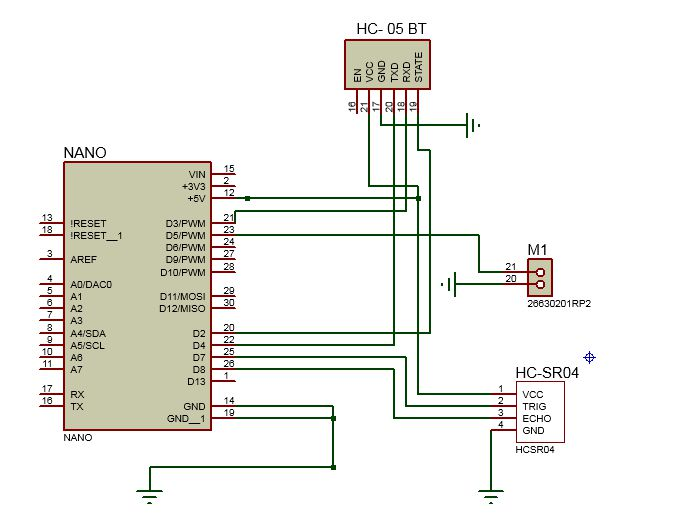
\includegraphics[width=.9\textwidth]{assets/conception1/img30.jpg}
    \caption{Circuit Proteus d'Arduino}
\end{figure}

\FloatBarrier

Après avoir fait le schéma, nous sommes passés à la conception d des circuits imprimés: Nous avons donc eu deux choix, soit celui d’utiliser le circuit imprimé pointillé traditionnel (figure a) ou le circuit imprimé (figure b). Nous avons donc choisi le deuxième choix simplement parce que c’est plus facile que le premier: il y a tellement de difficultés quand on travaille avec les circuits imprimés pointillés Ceux-ci relient les broches appropriées, évitant des  mal connexions et etc.

\begin{figure}[!htbp]
    \centering
    \begin{subfigure}[t]{.45\linewidth}
        \centering
         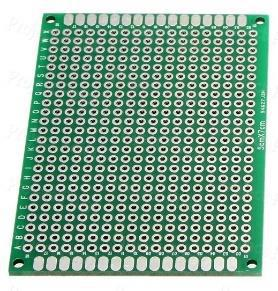
\includegraphics[width=\textwidth]{assets/conception1/img31.jpg}
        \caption{}
    \end{subfigure}
    \hfill
    \begin{subfigure}[t]{.45\linewidth}
        \centering
         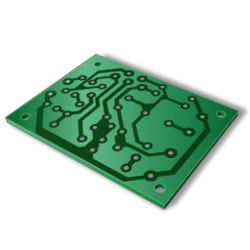
\includegraphics[width=\textwidth]{assets/conception1/img32.jpg}
         \caption{}
    \end{subfigure}
\end{figure}

\FloatBarrier

Sur Proteus nous passons au mode PCB layout et commençons à réaliser le circuit imprime en plaçant les composants utilisés dans le mode schematic capture, en choisissant le bon package* pour chaque composant et en faisant finalement les connexions en cuivre ... \\
Ci-dessous vous trouverez chaque composant avec le package fourni trouvé sur les bibliothèques Proteus

\begin{figure}[!htbp]
    \centering
    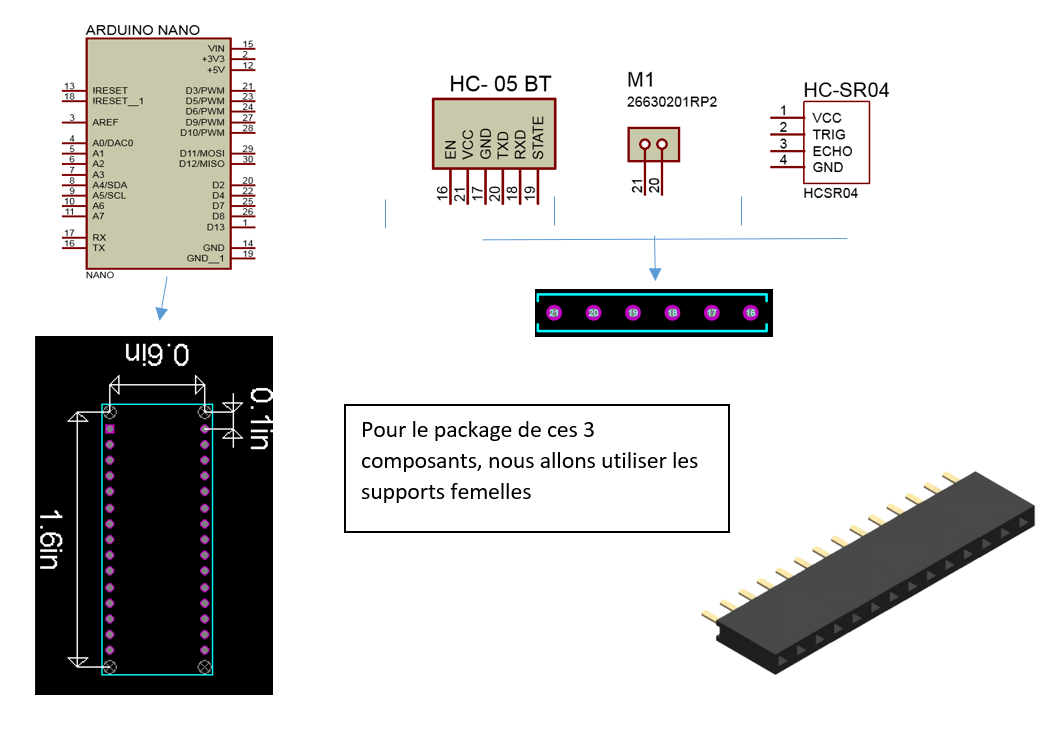
\includegraphics[width=\textwidth]{assets/conception1/2.png}
    \caption{Le package d'Arduino | Le support femelle}
\end{figure}

\FloatBarrier

Nous avons eu un problème avec le package du support fourni par la bibliothèque Proteus, la distance entre deux broches est de 0.54mm plus grande que celle que nous allons utiliser, nous devons soit modifier le package sur Isis puisqu’ils ont de mauvaises mesures ou nous pouvons faire notre propre à partir de zéro. \\
Nous avons trouvé SnapeDA comme un site fiable d’où nous obtenons des packages des composants, mais nous n’avons pas pu trouver les mesures correctes pour les supports, nous avons donc décidé de les faire.

\begin{figure}[!htbp]
    \centering
    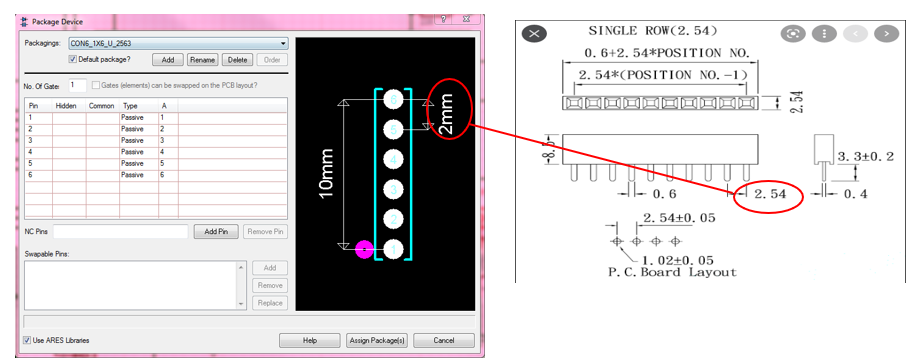
\includegraphics[width=\textwidth]{assets/conception1/1.png}
    \caption{Paramètres de support défaut de Proteus et les spécifications réelles}
\end{figure}

\FloatBarrier

Nous nous sommes retrouvés avec cet circuit et nous avons également utilisé le 3D Visualizer mode pour avoir une version 3d proche de la vie réelle de la carte de sorte que nous puissions travailler sur elle comme une base de notre conception de boîtier

\begin{figure}[!htbp]
    \centering
    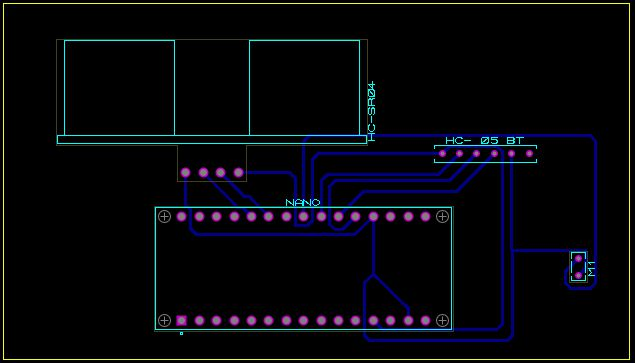
\includegraphics[width=.7\textwidth]{assets/conception1/img49.jpg}
    \caption{Layout du PCB du circuit Arduino}
\end{figure}

\begin{figure}[!htbp]
    \centering
    \includegraphics[width=.7\textwidth]{assets/conception1/img50.jpg}
    \caption{Modèle 3D du PCB du circuit Arduino}
\end{figure}

\FloatBarrier

Nous avons commencé à ajouter plus de composants dans le schéma : nous ne pouvions plus alimenter le moteur vibreur avec la broche d’Arduino car elle ne produit qu’un faible courant de 40mA et le moteur a besoin d’au moins 70ma de courant pour fonctionner correctement, également un de ces composants pourrait être endommagé en cours de route donc nous avons utilisé un moteur driver de référence l293d, nous avons aussi ajouté un moteur secondaire pour augmenter l’intensité de feedback

\begin{figure}[!htbp]
    \centering
    \includegraphics[width=\textwidth]{assets/conception1/img54.jpg}
    \caption{Circuit d'Arduino finale}
\end{figure}

\begin{figure}[!htbp]
    \centering
    \includegraphics[width=\textwidth]{assets/conception1/3.png}
    \caption{Le L293D}
\end{figure}

\begin{figure}[!htbp]
    \centering
    \includegraphics[width=.7\textwidth]{assets/conception1/img57.jpg}
    \caption{Le PCB du circuit Arduino avec le L293D}
\end{figure}

\begin{figure}[!htbp]
    \centering
    \includegraphics[width=.7\textwidth]{assets/conception1/img58.jpg}
    \caption{Modèle 3D PCB du circuit Arduino avec le L293D}
\end{figure}

\FloatBarrier

Et le dernier changement que nous avons fait concernant le circuit Arduino a été d’ajouter un buzzer, une lampe flash, et un interrupteur à glissière pour allumer/éteindre le circuit.
Nous avons également ajouté un support femelle qui va être connecté au circuit des boutons 

\begin{figure}[!htbp]
    \centering
    \includegraphics[width=\textwidth]{assets/conception1/img61.jpg}
\end{figure}

\FloatBarrier

Tous les nouveaux composants ajoutés utilisent les mêmes supports femelles qui ont été utilisés précédemment. Nous nous retrouvons avec le circuit ci-dessous

\begin{figure}[!htbp]
    \centering
    \includegraphics[width=\textwidth]{assets/conception1/img62.jpg}
    \caption{Le circuit final Arduino en Proteus}
\end{figure}

\begin{figure}[!htbp]
    \centering
    \includegraphics[width=\textwidth]{assets/conception1/img66.jpg}
    \caption{Layout du PCB final Arduino en Proteus}
\end{figure}

\begin{figure}[!htbp]
    \centering
    \includegraphics[width=\textwidth]{assets/conception1/img65.jpg}
    \caption{Modèle 3D du PCB final d'Arduino}
\end{figure}

\FloatBarrier

\subsubsection{Circuit des boutons}
\label{buttons-circuit-conception}
Quand nous avons commencé le processus de conception des PCB nous n’avions aucune idée du nombre de PCB qu’il y aura, nous voulions faire seulement un seul PCB qui va contenir tous les composants mais en conséquence il serait sorti grand en taille et qui va affecter considérablement la taille de la canne, et aussi la canne sera actionnée par l’utilisateur via des boutons de sorte qu’un PCB les contenant doit être proche de la surface supérieure de la canne, et en utilisant seulement un seul PCB n’aurait aucun sens , nous avons décidé alors de faire deux PCBs  \\
Nous allons maintenant parler du processus de fabrication !

Tout comme le circuit Arduino il y avait beaucoup de changements le long de la fabrication de ce circuit, le premier schéma à suivre était celui dessus

Nous avons utilisé 5 boutons pour exécuter différentes tâches pour faire fonctionner la canne, mais dans le schéma, nous pouvons remarquer que les boutons sont liés à l’arduino et nous avons mentionné plus tôt que l’arduino et les boutons sont séparé, C’est pourquoi nous avons connecté les boutons à un support qui sera connecté à ceux qui se trouve dans le circuit Arduino

\begin{figure}[!htbp]
    \centering
    \begin{subfigure}[t]{.45\linewidth}
        \centering
        \includegraphics[width=\textwidth]{assets/conception1/img71.jpg}
    \end{subfigure}
    \hfill
    \begin{subfigure}[t]{.45\linewidth}
        \centering
        \includegraphics[width=\textwidth]{assets/conception1/img73.jpg}
    \end{subfigure}
\end{figure}

\FloatBarrier

Quand nous avons voulu choisir les packages de chaque bouton nous allons utiliser dans le mode PCB layout nous n’avons pas pu trouver ceux appropriés dans la bibliothèque fournie qui va correspondre à ceux que nous allons utiliser et puisque les modèles de visualisation 3d vont être exportés et utilisés comme une base de conception 3d ils sont dû être précis \\
Nous avons utilisé des boutons-poussoirs momentanés : les 4 sur les côtés étaient gros et celui au milieu était petit afin que nous puissions économiser l’espace  le maximum possible  \\
Nous sommes allés à snapEDA pour télécharger l’empreinte et le modèle 3d des boutons et les utiliser dans le pcb layout


\begin{figure}[!htbp]
    \centering
    \includegraphics[width=\textwidth]{assets/conception1/4.png}
\end{figure}

\FloatBarrier

\begin{figure}[!htbp]
    \centering
    \begin{subfigure}[m]{.55\linewidth}
        \centering
        \includegraphics[width=\textwidth]{assets/conception1/img80.jpg}
    \end{subfigure}
    \hfill
    \begin{subfigure}[m]{.4\linewidth}
       La première version du circuit imprimé ressemblait à ceci, mais nous avons éventuellement apporté quelques changements
    \end{subfigure}
\end{figure}

\FloatBarrier

Deux leds ont été ajoutées : une pour indiquer batterie faible, et l’autre pour indiquer que la canne est sous tension 
Résistance supprimée : nous allons utiliser les résistances intégrées sur l’Arduino (la raison était mentionnée dans le chapitre précédent)

\begin{figure}[!htbp]
    \centering
    \begin{subfigure}[m]{.48\linewidth}
        \centering
        \includegraphics[width=\textwidth]{assets/conception1/img78.jpg}
    \end{subfigure}
    \hfill
    \begin{subfigure}[m]{.48\linewidth}
        \centering
        \includegraphics[width=\textwidth]{assets/conception1/img79.jpg}
    \end{subfigure}
\end{figure}

\begin{figure}[!htbp]
    \centering
    \includegraphics[width=.5\linewidth]{assets/conception1/img81.jpg}
\end{figure}

\FloatBarrier

Après avoir fini la conception des circuits imprimés nous avons fini avec ces deux modèles 3d

\begin{figure}[!htbp]
    \centering
    \begin{subfigure}[b]{.6\linewidth}
        \centering
        \includegraphics[width=\textwidth]{assets/conception1/img84.jpg}
    \end{subfigure}
    \hfill
    \begin{subfigure}[b]{.39\linewidth}
        \centering
        \includegraphics[width=\textwidth]{assets/conception1/img85.jpg}
    \end{subfigure}
\end{figure}

\FloatBarrier

Nous les utilisons en cours de fabrication de la canne dans le logiciel de conception 3D choisi!

\subsection{Conception 3D de bras}
Nous avons dû donner à nos pcbs une vie en leur donnant un boîtier afin que nous puissions assurer la portabilité et la convivialité du produit final : la canne intelligente.

D’abord nous avons pensé au polystyrène comme notre matière de base que nous allons faire notre canne, c’est un matériau léger, facilement accessible pour nous et aussi il nous a donné la capacité.

Pour le façonner comme notre souhait, mais nous n’étions pas entièrement satisfaits de ce matériau : il aurait l’air bon marché et amateur, nous voulions quelque chose de mieux, quelque chose qui correspondrait à la norme de l’industrie de la fabrication de produits de consommation à main : le plastique est le bon matériau.

Il existe beaucoup de techniques pour fabriquer des objets à partir de plastique, mais en tant qu’étudiants, nous ne pouvons pas aller avec les techniques complexes industrielles qui nécessitent des années d’expertises comme par exemple le moulage par injection:
Le procédé de moulage par injection consiste à chauffer et à injecter du plastique sous pression dans un outil de moulage métallique fermé, ce qui permet de fabriquer rapidement et à moindre coût des milliers, voire des millions de pièces identiques
le processus est expliqué étape par étape ci-dessous pour montrer la complexité de cette technique

\begin{figure}[!htbp]
    \centering
    \begin{subfigure}[m]{.55\linewidth}
        \centering
        \includegraphics[width=\textwidth]{assets/conception1/img90.jpg}
    \end{subfigure}
    \hfill
    \begin{subfigure}[m]{.4\linewidth}
       \paragraph*{Etape 1}
        Les granulés de la trémie alimentent le barillet chauffé et la vis rotative. \\
        Le matériau fondu par la chaleur, le frottement et la force de cisaillement est forcé par un clapet
    \end{subfigure}
\end{figure}

\begin{figure}[!htbp]
    \centering
    \begin{subfigure}[m]{.55\linewidth}
        \centering
        \includegraphics[width=\textwidth]{assets/conception1/img98.jpg}
    \end{subfigure}
    \hfill
    \begin{subfigure}[m]{.4\linewidth}
       \paragraph*{Etape 2}
        Après avoir été déplacée vers l’arrière par le plan de matière à l’avant, la vis est poussée vers l’avant par un bélier hydraulique.
    \end{subfigure}
\end{figure}

\begin{figure}[!htbp]
    \centering
    \begin{subfigure}[m]{.55\linewidth}
        \centering
        \includegraphics[width=\textwidth]{assets/conception1/img110.jpg}
    \end{subfigure}
    \hfill
    \begin{subfigure}[m]{.4\linewidth}
       \paragraph*{Etape 3}
        L’outil est maintenu fermé sous pression jusqu’à ce que le matériau plastique refroidisse et durcisse dans la cavité de l’outil de moule. \\
        C’est souvent la partie la plus longue du processus de moulage par injection
    \end{subfigure}
\end{figure}

\begin{figure}[!htbp]
    \centering
    \begin{subfigure}[m]{.55\linewidth}
        \centering
        \includegraphics[width=\textwidth]{assets/conception1/img113.jpg}
    \end{subfigure}
    \hfill
    \begin{subfigure}[m]{.4\linewidth}
       \paragraph*{Etape 4}
        La vis commence à reculer pour le prochain moulage. L’outil s’ouvre alors et la pièce plastique finie est éjectée. \\
        L’outil est fermé et le processus de moulage par injection recommence à 1.
    \end{subfigure}
\end{figure}

\FloatBarrier

Ce processus nécessite des machines spéciales de fabrication et en tant qu’étudiants, nous ne pouvons pas suivre cette procédure, c’est pourquoi nous avons opté pour l’impression 3D :

\subsubsection{Impression 3D}

\begin{figure}[!htbp]
    \centering
    \begin{subfigure}[m]{.55\linewidth}
        L’impression 3D ou la fabrication additive est un processus de fabrication d’objets solides tridimensionnels à partir d’un fichier numérique. \\
        La création d’un objet imprimé en 3D est réalisée à l’aide de processus additifs. Dans un processus additif, un objet est créé en posant des couches successives de matière jusqu’à ce que l’objet soit créé. Chacune de ces couches peut être vue comme une coupe transversale finement découpée de l’objet.
    \end{subfigure}
    \hfill
    \begin{subfigure}[m]{.4\linewidth}
        \centering
        \includegraphics[width=\textwidth]{assets/conception1/img116.jpg}
    \end{subfigure}
\end{figure}

\FloatBarrier

Le processus d’impression 3D commence par un modèle 3D qui est réalisé via un logiciel 3D habituellement appelé un logiciel CAD*  donc nous avons besoin d’un modèle 3D pour notre canne.

\begin{figure}[!htbp]
    \centering
    \includegraphics[width=\linewidth]{assets/conception1/img118.jpg}
\end{figure}

\FloatBarrier

Mais le problème est qu’en tant qu’équipe de deux membres aucun de nous ne sait comment faire de 3d design, nous aurions pu engager un designer pour faire le travail pour nous, mais cela n’aurait pas de sens puisque c’est notre projet de dernière année et  toutes les tâches doivent être faites par nos propres mains et cerveaux et c’est pourquoi nous nous sommes mis au défi et avons appris la conception 3d en moins d’un mois! 

Pour créer un modèle 3d, nous avons commencé avec des croquis 2d, nous avons dessiné comment nous avons imaginé la canne pour ressembler à un morceau de papier et tout comme les pcbs conception il y avait beaucoup de changements en cours de route, le premier croquis que nous avons trouvé était celui ci-dessous.

\begin{figure}[!htbp]
    \centering
    \includegraphics[width=\linewidth]{assets/conception1/img124.jpg}
    \caption{Sketch 2D de la première itération de la canne}
\end{figure}

\FloatBarrier

Vous pouvez voir dans ce croquis le plan supérieur des deux côtés et une vue isométrique, après le croquis 2d nous avons dû voir à quoi ça ressemblerait en 3d donc nous passons au logiciel CAD

\begin{figure}[!htbp]
    \centering
    \begin{subfigure}[m]{.22\linewidth}
        \centering
        \includegraphics[width=\textwidth]{assets/conception1/img125.jpg}
    \end{subfigure}
    \hfill
    \begin{subfigure}[m]{.22\linewidth}
        \centering
        \includegraphics[width=\textwidth]{assets/conception1/img127.jpg}
    \end{subfigure}
    \hfill
    \begin{subfigure}[m]{.22\linewidth}
        \centering
        \includegraphics[width=\textwidth]{assets/conception1/img129.jpg}
    \end{subfigure}
    \hfill
    \begin{subfigure}[m]{.22\linewidth}
        \centering
        \includegraphics[width=\textwidth]{assets/conception1/img131.jpg}
    \end{subfigure}
\end{figure}

\FloatBarrier

Il y avait quelques critères que nous avons fait que le logiciel devait avoir afin que nous puissions travailler avec lui :

\begin{enumerate}
    \item Le logiciel devait être interopérable avec notre logiciel de conception de cartes Proteus, de sorte que les modèles 3D exportés puissent y être importés et prêts à fonctionner.
    \item Il devrait y avoir un soutien en ligne actif / communauté afin que nous puissions trouver des solutions à tous les problèmes / difficultés que nous allons faire face le long du chemin faisant la canne.
    \item . Enfin, il faut qu’il y ait une version piratée sur Internet, car nous n’avons pas les moyens de payer le coût de propriété de l’application. La plupart des options correspondaient à notre liste de critères, mais nous avons choisi SOLIDWORKS car nous avons trouvé l’interface utilisateur facile à comprendre et pas compliquée. 
\end{enumerate}

\begin{figure}[!htbp]
    \centering
    \includegraphics[width=\linewidth]{assets/conception1/img135.jpg}
\end{figure}

\FloatBarrier

Après avoir choisi un logiciel CAD nous avons fait le premier modèle 3d de la canne juste pour donner à notre  croquis 2d un peu de vie.

\begin{figure}[!htbp]
    \centering
    \includegraphics[width=\linewidth]{assets/conception1/img138.jpg}
\end{figure}

\FloatBarrier

Le bouton du milieu n’a pas été inclus sur le 2d ou le croquis 3D car il a été fait avant que nous ayons  ajouté le bouton dans notre circuit. \\
Maintenant, nous avons commencé à travailler avec des mesures réelles basées sur les principaux composants utilisés dans la canne : la batterie lipo et les deux circuits 
Nous avons dessiné le croquis en 2d

\begin{figure}[!htbp]
    \centering
    \includegraphics[width=\linewidth]{assets/conception1/5.png}
\end{figure}

\FloatBarrier

Puis nous l’avons réalisé en 3d : nous avons d’abord dû concevoir la batterie que nous allons utiliser parce qu’elle sera le point de départ de notre conception (le circuit Arduino et les boutons aussi, mais le modèle 3d est déjà fait en Proteus)

\begin{figure}[!htbp]
    \centering
    \begin{subfigure}[m]{.55\linewidth}
        \centering
        \includegraphics[width=\textwidth]{assets/conception1/img142.jpg}
    \end{subfigure}
    \hfill
    \begin{subfigure}[m]{.3\linewidth}
        \centering
        \includegraphics[width=\textwidth]{assets/conception1/img143.jpg}
    \end{subfigure}
\end{figure}

\FloatBarrier

après, nous concevons la partie inférieure

\begin{figure}[!htbp]
    \centering
    \includegraphics[width=\linewidth]{assets/conception1/img144.jpg}
\end{figure}

\FloatBarrier

Nous montons ensuite la batterie et les modèles arduino sur la partie inférieure

\begin{figure}[!htbp]
    \centering
    \includegraphics[width=\linewidth]{assets/conception1/6.png}
\end{figure}

\FloatBarrier

Les boutons pcb doivent être accessibles à la main de l’utilisateur à elle doivent être situés dans la partie supérieure de la canne

\begin{figure}[!htbp]
    \centering
    \includegraphics[width=.45\linewidth]{assets/conception1/img153.jpg}
    \caption{Première version du modèle 3d du circuit imprimé des boutons dans SolidWorks}
\end{figure}

\FloatBarrier

Nous avons donc fait une partie supérieure qui tiendrait ce circuit imprimé et en même temps être sur la partie inférieure pour former une forme solide ensemble

\begin{figure}[!htbp]
    \centering
    \includegraphics[width=.9\linewidth]{assets/conception1/img154.jpg}
    \caption{Première version du modèle 3D de la bras}
\end{figure}


\begin{figure}
    \begin{subfigure}[m]{.55\linewidth}
        Les boutons que nous avons utilisés (ceux sur les côtés) étaient inclus avec des bouchons (figure a) ,nous avons dû concevoir les mêmes bouchons afin pour pouvoir les inclure dans le modèle 3d de circuit des boutons 
    \end{subfigure}
    \begin{subfigure}[m]{.4\linewidth}
        \centering
        \includegraphics[width=\textwidth]{assets/conception1/img158.jpg}
        \caption{}
    \end{subfigure}
\end{figure}


\begin{figure}
    \begin{subfigure}[m]{.65\linewidth}
        \includegraphics[width=\textwidth]{assets/conception1/img160.jpg}
        \caption{Les mesures sont exactement comme celles utilisées dans la vie réelle.}
    \end{subfigure}
    \hfill
    \begin{subfigure}[m]{.25\linewidth}
        \centering
        \includegraphics[width=\textwidth]{assets/conception1/img159.jpg}
        \caption{}
        \includegraphics[width=\textwidth]{assets/conception1/img161.jpg}
        \caption{}
    \end{subfigure}
\end{figure}

\FloatBarrier

Après avoir fini les bouchons, nous les avons montés sur le dessus de la carte comme ils sont dans la vraie vie

\begin{figure}[!htbp]
    \centering
    \includegraphics[width=.6\linewidth]{assets/conception1/img157.jpg}
    \caption{Circuit boutons 3d avec les bouchons}
\end{figure}

\FloatBarrier

Puis on a tout monté et on a fini avec ça

\begin{figure}
    \begin{subfigure}[m]{.48\linewidth}
        \centering
        \includegraphics[width=\textwidth]{assets/conception1/img165.jpg}
    \end{subfigure}
    \hfill
    \begin{subfigure}[m]{.48\linewidth}
        \centering
        \includegraphics[width=\textwidth]{assets/conception1/img164.jpg}
    \end{subfigure}
    \caption{Première itération du bras}
\end{figure}

\FloatBarrier

Notre premier design 3D est terminé et il semble incroyable… !\\
Non, ce n’est certainement pas étonnant, nous n’avons pas aimé le résultat que nous voyions : ce n’était pas attrayant comme nous l’avions prévu, c’était lourd, ennuyeux et dans l’ensemble ne valait pas l’impression 3D.

Nous avons pris une pause car nous avons mis beaucoup d’efforts dans la conception ci-dessous (il n’a peut-être pas aimé qu’il ait fallu beaucoup d’effort à faire, mais nous n’avions aucune expérience donc nous avons dû apprendre les techniques et les bases dès que possible pour réaliser que mais apparemment ce n’était pas assez)  \\
Nous avons donc pris une semaine qui a était dédié pour apprendre des techniques plus avancées qui nous aideront à réaliser notre vision.

La base de notre conception 3d (parties supérieure et inférieure) était ce coquis ci-dessous

\begin{figure}
    \begin{subfigure}[m]{.65\linewidth}
        \centering
        \includegraphics[width=\textwidth]{assets/conception1/img168.jpg}
    \end{subfigure}
    \hfill
    \begin{subfigure}[m]{.3\linewidth}
        La partie supérieure a dû être commencée de ce croquis et la même chose s’applique à la partie inférieure. \\
        Commençons par la partie inférieure car c’est celle qui va contenir la plupart des composants. \\
        Le problème avec la première version était qu’elle ressemblait à une boîte ! \\
        Il ne ressemblait pas à quelque chose qui a été fait pour être portable, et il serait certainement laisser quelques cicatrices sur la main de tout utilisateur qui le détient pendant un certain temps.
    \end{subfigure}
\end{figure}

\FloatBarrier

Des courbures étaient nécessaires dans la conception pour la rendre plus ergonomique

\begin{figure}[!htbp]
    \centering
    \includegraphics[width=.9\linewidth]{assets/conception1/img169.jpg}
\end{figure}

Cette courbure va être au milieu de la partie inférieure, et le long d’autres courbures sur le côté, il va donner le plus bas une meilleure forme.

\begin{figure}
    \begin{subfigure}[m]{.65\linewidth}
        \centering
        \includegraphics[width=\textwidth]{assets/conception1/img173.jpg}
    \end{subfigure}
    \hfill
    \begin{subfigure}[m]{.3\linewidth}
        \centering
        \includegraphics[width=\textwidth]{assets/conception1/img172.jpg}
    \end{subfigure}
\end{figure}

\FloatBarrier

Nous ne faisons les courbes latérales que d’un côté car nous allons utiliser une fonctionnalité dans SOLIDWORKS appelée « miroir », cela signifie essentiellement que nous pouvons reproduire des croquis d’un côté à l’autre .

\begin{figure}
    \begin{subfigure}[m]{.55\linewidth}
        \centering
        \includegraphics[width=\textwidth]{assets/conception1/img175.jpg}
        \vspace{0.5cm}
        \includegraphics[width=\textwidth]{assets/conception1/img176.jpg}
    \end{subfigure}
    \hfill
    \begin{subfigure}[m]{.4\linewidth}
        \centering
        \includegraphics[width=\textwidth]{assets/conception1/img174.jpg}
    \end{subfigure}
\end{figure}

\FloatBarrier

\begin{figure}[!htbp]
    \centering
    \includegraphics[width=\linewidth]{assets/conception1/img179.jpg}
\end{figure}

\begin{figure}[!htbp]
    \centering
    \includegraphics[width=\linewidth]{assets/conception1/img180.jpg}
\end{figure}

\FloatBarrier

C’est ce que nous finissons avec après le miroir , la partie est creuse de l’intérieur parce qu’il doit adapter les composants

Soulignons les principales différences entre les deux versions de la partie inférieure!

\begin{figure}[!htbp]
    \centering
    \includegraphics[width=\linewidth]{assets/conception1/8.png}
\end{figure}

\FloatBarrier

Donc la différence la plus évidente est que la deuxième version a plus de courbes par rapport à la première et qui lui a donné plus le sentiment de produits de consommation (télécommande).

En outre, il y a une différence de hauteur de 4cm qui le rendent la partie inférieure sur tout moins lourd.

\begin{figure}[!htbp]
    \centering
    \includegraphics[width=\linewidth]{assets/conception1/10.png}
\end{figure}

\FloatBarrier

Et par moins lourd on entend une diminution de presque 70 gr entre les deux versions.

Nous devons faire des espaces pour les composants utilisés dans la canne, nous avons commencé avec la batterie lipo.

\begin{figure}[!htbp]
    \centering
    \begin{subfigure}{.6\linewidth}
        \centering
        \includegraphics[width=\linewidth]{assets/conception1/img190.jpg}
    \end{subfigure}
    \hfill
    \begin{subfigure}[m]{.3\linewidth}
        Pour tenir la batterie à sa place, nous devons faire un plateau et coller la batterie sur elle afin que nous puissions éviter tout type de mouvements indésirables
    \end{subfigure}
\end{figure}

\FloatBarrier

\begin{figure}[!htbp]
    \centering
    \begin{subfigure}{.5\linewidth}
        \centering
        \includegraphics[width=\linewidth]{assets/conception1/img193.jpg}
    \end{subfigure}
    \hfill
     \begin{subfigure}{.45\linewidth}
        \centering
        \includegraphics[width=\linewidth]{assets/conception1/img196.jpg}
    \end{subfigure}
\end{figure}

\FloatBarrier

\begin{figure}[!htbp]
    \centering
    \begin{subfigure}{.6\linewidth}
        \centering
        \includegraphics[width=\linewidth]{assets/conception1/img195.jpg}
    \end{subfigure}
    \hfill
    \begin{subfigure}[m]{.3\linewidth}
       C’est le plateau dont nous avons besoin, il a 3 supports et sera préfet pour adapter la batterie sans se croiser avec la partie supérieure 
    \end{subfigure}
\end{figure}

\FloatBarrier

\begin{figure}[!htbp]
    \centering
    \includegraphics[width=\linewidth]{assets/conception1/11.png}
\end{figure}

\FloatBarrier

\begin{figure}[!htbp]
    \centering
    \includegraphics[width=\linewidth]{assets/conception1/img201.jpg}
\end{figure}

\FloatBarrier

\begin{figure}[!htbp]
    \centering
    \includegraphics[width=.5\linewidth]{assets/conception1/img200.jpg}
\end{figure}

\FloatBarrier

Maintenant, nous montons l’arduino pcb dans la partie inférieure.

\begin{figure}[!htbp]
    \centering
    \includegraphics[width=\linewidth]{assets/conception1/12.png}
\end{figure}

\FloatBarrier

Il y avait deux possibilités de montage du circuit Arduino: il devait soit être orienté vers le haut, soit vers le bas.

\begin{figure}[!htbp]
    \centering
    \includegraphics[width=\linewidth]{assets/conception1/img215.jpg}
\end{figure}

\FloatBarrier

Il peut être monté comme ceci mais il y avait deux inconvénients avec cette façon :

\begin{enumerate}
    \item Nous ne profiterions pas de cette courbure qui a été faite en premier lieu pour rendre la canne confortable sur la paume de la main.
    \begin{figure}[!htbp]
        \centering
        \includegraphics[width=.6\linewidth]{assets/conception1/13.png}
    \end{figure}
    \FloatBarrier
    \item L’Arduino a une certaine hauteur et il affectera la hauteur de la partie supérieure.
    \begin{figure}[!htbp]
        \centering
        \includegraphics[width=.6\linewidth]{assets/conception1/14.png}
    \end{figure}
    \FloatBarrier
\end{enumerate}

C’est pourquoi nous allons le monter face vers le bas, nous allons d’abord faire quelques trous de fixation pour visser le circuit imprimé en place ! 

\begin{figure}[!htbp]
    \centering
    \begin{subfigure}{.5\linewidth}
        \centering
        \includegraphics[width=\linewidth]{assets/conception1/img213.jpg}
    \end{subfigure}
    \hfill
     \begin{subfigure}{.4\linewidth}
        \centering
        \includegraphics[width=\linewidth]{assets/conception1/img214.jpg}
    \end{subfigure}
\end{figure}

\FloatBarrier

\begin{figure}[!htbp]
    \centering
    \begin{subfigure}{.65\linewidth}
        \centering
        \includegraphics[width=\linewidth]{assets/conception1/img216.jpg}
    \end{subfigure}
    \hfill
    \begin{subfigure}[m]{.3\linewidth}
        Nous avons remarqué après le montage du circuit imprimé qu’il touche la surface de la partie inférieure. \\
        Nous avons ensuite redessiné la forme de la partie inférieure (la courbure centrale précisément ) de sorte qu’il peut adapter le circuit imprimé principal sans aucune frotement
    \end{subfigure}
\end{figure}

\FloatBarrier

\begin{figure}[!htbp]
    \centering
    \begin{subfigure}[m]{.6\linewidth}
        Après avoir fini la carte, nous devons maintenant monter l’interrupteur d’alimentation. \\
        Nous allons utiliser un commutateur à glissière (figure) \\
        Nous avons cherché un modèle 3D pour l’utiliser dans solidworks de GRABCAD \\
        Et nous en avons trouvé un qui correspond au nôtre. \\
    \end{subfigure}
    \hfill
    \begin{subfigure}{.3\linewidth}
        \centering
        \includegraphics[width=\linewidth]{assets/conception1/img221.jpg}
        \includegraphics[width=\linewidth]{assets/conception1/img222.jpg}
    \end{subfigure}
\end{figure}

\FloatBarrier

\begin{figure}[!htbp]
    \centering
    \begin{subfigure}[m]{.6\linewidth}
        \centering
        \includegraphics[width=\linewidth]{assets/conception1/img223.jpg}
    \end{subfigure}
    \hfill
    \begin{subfigure}{.3\linewidth}
        \centering
        \includegraphics[width=\linewidth]{assets/conception1/img224.jpg}
    \end{subfigure}
\end{figure}

\FloatBarrier

Maintenant, nous avons terminé la partie inférieure et monté toutes les pièces : batterie, circuit Arduino et le commutateur.

Nous allons maintenant passer à la partie supérieure et tout comme la partie inférieure, nous allons commencer par le croquis 2d de base.

\begin{figure}[!htbp]
    \centering
          \begin{subfigure}{.45\linewidth}
                \centering
                \includegraphics[width=\linewidth]{assets/conception1/img227.jpg}
            \end{subfigure}
            \hfill
            \begin{subfigure}[m]{.45\linewidth}
                \centering
                \includegraphics[width=\linewidth]{assets/conception1/img228.jpg}
            \end{subfigure}
        \end{figure}  
        
\FloatBarrier

Nous avons suivi la même approche de la partie supérieure, nous avons fait une courbure qui est orientée vers le haut cette fois, nous avons essayé de garder simple et l’avant a dû être plus grand que le reste de la boddy car il tiendra le capteur à ultrasons.

Des courbures latérales ont été faites pour façonner la surface de la pièce.


\begin{figure}[!htbp]
    \centering
    \includegraphics[width=\linewidth]{assets/conception1/15.png}
\end{figure}

\FloatBarrier

\begin{figure}[!htbp]
    \centering
    \begin{subfigure}[m]{.2\linewidth}
        On a fini avec un corps qui ressemble à ça. \\
        Mais un gros problème s’est posé quand nous avons essayé d’y monter des pièces .
    \end{subfigure}
    \hfill
    \begin{subfigure}{.75\linewidth}
        \centering
        \includegraphics[width=\linewidth]{assets/conception1/img236.jpg}
    \end{subfigure}
\end{figure}

\begin{figure}[!htbp]
    \centering
    \begin{subfigure}[m]{.2\linewidth}
       Pour une raison quelconque, cette approche de faire des courbures et de créer une surface d’eux afin que nous puissions avoir un corps solide à la fin ne fonctionnait pas de notre côté comme la partie inférieure.
    \end{subfigure}
    \hfill
    \begin{subfigure}{.75\linewidth}
        \centering
        \includegraphics[width=\linewidth]{assets/conception1/img235.jpg}
    \end{subfigure}
\end{figure}

\begin{figure}[!htbp]
    \centering
    \includegraphics[width=\linewidth]{assets/conception1/16.png}
\end{figure}

\FloatBarrier

\begin{figure}[!htbp]
    \centering
    \begin{subfigure}[m]{.2\linewidth}
       On fait une coupe latérale et on peut voir l’espace vide entre la douille et le corps de la pièce
    \end{subfigure}
    \hfill
    \begin{subfigure}{.75\linewidth}
        \centering
        \includegraphics[width=\linewidth]{assets/conception1/img261.jpg}
    \end{subfigure}
\end{figure}

\begin{figure}[!htbp]
    \centering
    \includegraphics[width=.7\linewidth]{assets/conception1/17.png}
\end{figure}

\FloatBarrier

Nous avons essayé de trouver une solution dans la communauté SOLIDWORKS, mais nous n’en avons pas trouvé. \\
Nous devons changer l’approche et concevoir la partie supérieure d’une autre façon. \\
Alors au lieu de courbures, faisons un corps solide à partir du croquis de base 2d! \\

\begin{figure}[!htbp]
    \centering
    \includegraphics[width=.7\linewidth]{assets/conception1/img269.jpg}
\end{figure}

\FloatBarrier

Ensuite, nous allons faire des coupes dans le corps solide jusqu’à ce que nous sommes satisfaits des résultats.

Commençons par la première coupe : 

\begin{figure}[!htbp]
    \centering
    \includegraphics[width=\linewidth]{assets/conception1/18.png}
\end{figure}

\FloatBarrier

La pièce était un corps solide nous avons enlevé le matériel à l’intérieur afin que nous puissions monter nos pièces

\begin{figure}[!htbp]
    \centering
    \includegraphics[width=\linewidth]{assets/conception1/19.png}
\end{figure}

\FloatBarrier

Nous allons maintenant commencer à monter la première partie dans la partie supérieure après nous être assurés qu’il n’y a pas de problèmes comme la partie précédente.

nous avons commencé avec le capteur à ultrasons


\begin{figure}[!htbp]
    \centering
    \includegraphics[width=\linewidth]{assets/conception1/20.png}
\end{figure}

\begin{figure}[!htbp]
    \centering
    \includegraphics[width=\linewidth]{assets/conception1/img310.jpg}
\end{figure}

\FloatBarrier

Voici à quoi ressemble le résultat final de la socket. 
Le capteur HC-SR04 peut maintenant s’insérer parfaitement dans la partie supérieure de la canne

\begin{figure}[!htbp]
    \centering
    \includegraphics[width=.8\linewidth]{assets/conception1/img311.jpg}
\end{figure}

\FloatBarrier

\begin{figure}[!htbp]
    \centering
    \includegraphics[width=\linewidth]{assets/conception1/22.png}
\end{figure}

\FloatBarrier

\begin{figure}[!htbp]
    \centering
    \includegraphics[width=\linewidth]{assets/conception1/24.png}
\end{figure}

\FloatBarrier

On se déplace ensuite pour monter les boutons pcb et buzzer place.

\begin{figure}[!htbp]
    \centering
    \includegraphics[width=\linewidth]{assets/conception1/25.png}
\end{figure}

\FloatBarrier

\begin{figure}[!htbp]
    \centering
    \includegraphics[width=\linewidth]{assets/conception1/26.png}
\end{figure}

\FloatBarrier

Nous sommes passés à la partie supérieure, et tout comme la carte Arduino, l’autre circuit doit être monté et vissé sur la partie supérieure.  

\begin{figure}[!htbp]
    \centering
    \includegraphics[width=\linewidth]{assets/conception1/27.png}
\end{figure}

\FloatBarrier

\begin{figure}[!htbp]
    \centering
    \includegraphics[width=\linewidth]{assets/conception1/28.png}
\end{figure}

\FloatBarrier

\begin{figure}[!htbp]
    \centering
    \begin{subfigure}[m]{.2\linewidth}
       Voilà à quoi tout ressemblait !
    \end{subfigure}
    \hfill
    \begin{subfigure}{.75\linewidth}
        \centering
        \includegraphics[width=\linewidth]{assets/conception1/img332.jpg}
    \end{subfigure}
\end{figure}

\FloatBarrier

Nous avons ensuite fait une place pour le buzzer avec des trous de sorte que les sons peuvent être entendus clairement, nous avons ajouté deux places pour les moteurs sur les deux côtés de la partie supérieure des murs. \\
Et finalement, nous avons fait une place pour la LED flash et un endroit où wo va monter le circuit de charge. 

\begin{figure}[!htbp]
    \centering
    \begin{subfigure}[m]{.3\linewidth}
        \includegraphics[width=\linewidth]{assets/conception1/img333.jpg}
    \end{subfigure}
    \hfill
    \begin{subfigure}[m]{.3\linewidth}
        \includegraphics[width=\linewidth]{assets/conception1/img334.jpg}
    \end{subfigure}
    \hfill
    \begin{subfigure}[m]{.3\linewidth}
        \includegraphics[width=\linewidth]{assets/conception1/img335.jpg}
    \end{subfigure}
\end{figure}

\FloatBarrier

Les bords de la partie supérieure étaient trop pointus et agressifs pour ce type de produit, la canne devait être lisse \\
Il manquait aussi un caractère, nous avons donc ajouté quelques détails.

\begin{figure}[!htbp]
    \centering
    \includegraphics[width=.5\linewidth]{assets/conception1/img338.jpg}
\end{figure}

\FloatBarrier

Chaque produit a un nom au dos ou sur l’un de ses côtés, il se présente à celui qui le porte, notre produit n’a pas de nom aucune identification, nous avons dû le changer donc nous avons gravé au dos de la partie inférieure le nom que nous avons trouvé : « guideme »
Nous avons également inclus nos noms en tant que fondateurs de ces produits et le contexte de sa réalisation qui est le projet de dernière année.

\begin{figure}[!htbp]
    \centering
    \includegraphics[width=.8\linewidth]{assets/conception1/img342.jpg}
\end{figure}

\FloatBarrier

\begin{figure}[!htbp]
    \centering
    \includegraphics[width=\linewidth]{assets/conception1/img349.jpg}
\end{figure}

\FloatBarrier

\begin{figure}[!htbp]
    \centering
    \includegraphics[width=\linewidth]{assets/conception1/img348.jpg}
\end{figure}